%% ----------------------------------------------------------------
%% Thesis.tex -- MAIN FILE (the one that you compile with LaTeX)
%% ---------------------------------------------------------------- 

\documentclass[12pt]{ucthesis}
% \graphicspath{{Figures/}}  % Location of the graphics files (set up for graphics to be in PDF format)

% Include any extra LaTeX packages required
\usepackage[square, numbers, comma, sort&compress]{natbib}  % Use the "Natbib" style for the references in the Bibliography
\usepackage{verbatim}  % Needed for the "comment" environment to make LaTeX comments
\usepackage{vector}  % Allows "\bvec{}" and "\buvec{}" for "blackboard" style bold vectors in maths
% \hypersetup{urlcolor=blue, colorlinks=true}  % Colours hyperlinks in blue, but this can be distracting if there are many links.
\usepackage{url}
\usepackage{graphicx}
\usepackage[pdftex,plainpages=false,breaklinks=true,colorlinks=true,urlcolor=blue,citecolor=blue,%
				    linkcolor=blue,bookmarks=true,bookmarksopen=true,%
				    bookmarksopenlevel=3,pdfstartview=FitV,
				    pdfauthor={Truman E. Ellis},
				    pdftitle={High Order Finite Elements for Lagrangian Computational Fluid Dynamics},
				    pdfkeywords={thesis, masters, cal poly}
				    ]{hyperref}
%Options with pdfstartview are FitV, FitB and FitH
\pdfcompresslevel=1
\usepackage{amssymb,amsmath}
\usepackage[letterpaper]{geometry}
\usepackage[overload]{textcase}
\usepackage{fancyhdr}
\usepackage{setspace}  
\usepackage{longtable}
\usepackage[absolute]{textpos}
\usepackage[tight]{subfigure}
\usepackage{changepage}
\setlength{\TPHorizModule}{\paperwidth}\setlength{\TPVertModule}{\paperheight}


\bibliographystyle{abbrv}

\setlength{\parindent}{0.25in} \setlength{\parskip}{6pt}

\geometry{verbose,nohead,tmargin=1.25in,bmargin=1in,lmargin=1.5in,rmargin=1.3in}

\setcounter{tocdepth}{2}


% Different font in captions (single-spaced, bold) ------------
\newcommand{\captionfonts}{\small\bf\ssp}

\makeatletter  % Allow the use of @ in command names
\long\def\@makecaption#1#2{%
  \vskip\abovecaptionskip
  \sbox\@tempboxa{{\captionfonts #1: #2}}%
  \ifdim \wd\@tempboxa >\hsize
    {\captionfonts #1: #2\par}
  \else
    \hbox to\hsize{\hfil\box\@tempboxa\hfil}%
  \fi
  \vskip\belowcaptionskip}
\makeatother   % Cancel the effect of \makeatletter

\def\newblock{\hskip .11em plus .33em minus .07em}
% ---------------------------------------

% \newcommand\btypeout[1]{\bhrule\typeout{\space #1}\bhrule}
% % \newcommand\addtotoc[1]{
% % \refstepcounter{dummy}
% % \addcontentsline{toc}{chapter}{#1}}
% \newcommand\listsymbolname{Nomenclature}
% \usepackage{longtable}
% \newcommand\listofsymbols[2]{
% % \btypeout{\listsymbolname}
% % \addtotoc{\listsymbolname}
%     \chapter*{\listsymbolname}
% %       \@mkboth{
% %           \MakeUppercase\listsymbolname}{\MakeUppercase\listsymbolname}}
% \begin{longtable}[c]{#1}#2\end{longtable}\par
%     \cleardoublepage
% }

%=============================================================================
%                              Useful Commands
%=============================================================================

% ===== Rob Rieben's Useful Commands =====
 
\newcommand{\refEq}[1]{(\ref{eq:#1})}
\newcommand{\refChap}[1]{Chapter~\ref{chap:#1}}
\newcommand{\refFig}[1]{Figure~\ref{fig:#1}}
\newcommand{\refSec}[1]{Section~\ref{sec:#1}}
\newcommand{\refTab}[1]{Table~\ref{tab:#1}}
\newcommand{\refApp}[1]{Appendix~\ref{app:#1}}
\newcommand{\newEq}[2]{\begin{equation} \label{eq:#1} #2 \end{equation}}

\newcommand{\el}[2]{$#1$-$#2$}
\newcommand{\SedovPlot}[5]{
\clearpage
\newpage
\begin{figure}[ht]
\begin{textblock*}{7in}(.75in,1in)
\centering
\subfigure[Velocity magnitude pseudocolor plot (\textit{left}). Velocity magnitude scatter plot compared to exact solution (\textit{right}).]{
\includegraphics[width=7in,keepaspectratio=true]{./Figures/SedovV_#1_#2x#2_hg#3}
\label{fig:SedovV_#1_#2x#2_hg#3}
}
\subfigure[Density pseudocolor plot (\textit{left}). Density scatter plot compared to exact solution (\textit{right}).]{
\includegraphics[width=7in,keepaspectratio=true]{./Figures/SedovD_#1_#2x#2_hg#3}
\label{fig:SedovD_#1_#2x#2_hg#3}
}
\caption{Sedov explosion problem on #2$\times$#2 mesh using #4 elements #5 hourglass filtering}
\label{fig:Sedov_#1_#2x#2_hg#3}
\end{textblock*}
\end{figure}
\clearpage
\newpage}

\newcommand{\NohPlot}[5]{
\clearpage
\newpage
\begin{figure}[ht]
\begin{textblock*}{7in}(.75in,1in)
\centering
\subfigure[Velocity magnitude pseudocolor plot (\textit{left}). Velocity magnitude scatter plot compared to exact solution (\textit{right}).]{
\includegraphics[width=7in,keepaspectratio=true]{./Figures/NohV_#1_#2x#2_hg#3}
\label{fig:NohV_#1_#2x#2_hg#3}
}
\subfigure[Density pseudocolor plot (\textit{left}). Density scatter plot compared to exact solution (\textit{right}).]{
\includegraphics[width=7in,keepaspectratio=true]{./Figures/NohD_#1_#2x#2_hg#3}
\label{fig:NohD_#1_#2x#2_hg#3}
}
\caption{Noh explosion problem on #2$\times$#2 mesh using #4 elements #5 hourglass filtering}
\label{fig:Noh_#1_#2x#2_hg#3}
\end{textblock*}
\end{figure}
\clearpage
\newpage}

\newcommand{\SaltzmanPlot}[5]{
\clearpage
\newpage
\begin{figure}[ht]
\begin{textblock*}{7in}(.75in,1in)
\centering
\subfigure[Pseudocolor plot of $x$-velocity (\textit{left}). Scatter plot of $x$-velocity (\textit{right}).]{
\includegraphics[width=7in,keepaspectratio=true]{./Figures/SaltzmanV_#1_50x10_hg#3}
\label{fig:SaltzmanV_#1_50x10_hg#3}
}
\subfigure[Density pseudocolor plot (\textit{left}). Density scatter plot (\textit{right}).]{
\includegraphics[width=7in,keepaspectratio=true]{./Figures/SaltzmanD_#1_50x10_hg#3}
\label{fig:SaltzmanD_#1_50x10_hg#3}
}
\caption{Saltzman piston problem on 50$\times$10 mesh using #4 elements #5 hourglass filtering at t=0.925}
\label{fig:Saltzman_#1_50x10_hg#3}
\end{textblock*}
\end{figure}
\clearpage
\newpage}

%=============================================================================
%                        Common Shortcut Definitions
%=============================================================================
%== Text mode defines ==
\def\Elem{$\Sigma$ }
\def\Pspace{$\mathcal{P}$ }
\def\Dof{$\mathcal{A}$ }
\def\FE{$(\Sigma, \mathcal{P}, \mathcal{A})$ }
\def\Hdiv{$H(Div)$ }
\def\Hcurl{$H(Curl)$ }
\def\RefHex{$\hat{\Sigma}$ }
\def\IntRule{${\mathcal Q}$ }
%== Math mode defines ==
\def\Grad{\vec \nabla}
\def\Curl{\vec \nabla \times}
\def\Div{\vec \nabla \cdot}
\def\VecLaplacian{\vec \nabla^2}
 

\begin{document}

% Declarations for Front Matter

% Update fields below!
\title{High Order Finite Elements for Lagrangian Computational Fluid Dynamics}
\author{Truman E. Ellis}
\degreemonth{April} \degreeyear{2010} \degree{Master of Science}
\defensemonth{April} \defenseyear{2010}
\numberofmembers{5} \chair{Faisal Kolkailah, Ph.D.} \othermemberA{Robert Rieben, Ph.D.} \othermemberB{Tzanio Kolev, Ph.D.} \othermemberC{David Marshall, Ph.D.} \othermemberD{Alberto Jimenez, Ph.D.} \field{Aerospace Engineering} \campus{San Luis Obispo}
\copyrightyears{seven}



\maketitle

\begin{frontmatter}

% Custom made for Cal Poly (by Mark Barry, modified by Andrew Tsui).
\copyrightpage

% Custom made for Cal Poly (by Andrew Tsui).
\committeemembershippage

\begin{abstract}

A general finite element method is presented to solve the Euler equations in a Lagrangian reference frame. This FEM framework allows for separate arbitrarily high order representation of kinematic and thermodynamic variables. An accompanying hydrodynamics code written in Matlab is presented as a test-bed to experiment with various basis function choices. A wide range of basis function pairs are postulated and a few choices are developed further, including the bi-quadratic \el{Q_2}{\hat Q_1} and \el{Q_2}{\hat Q_2} elements. These are compared with a corresponding pair of low order bi-linear elements, traditional \el{Q_1}{Q_0} and sub-zonal pressure \el{Q_1}{\hat Q_1}. Several test problems are considered including static convergence tests, the acoustic wave hourglass test, the Sod shocktube, the Noh implosion problem, the Saltzman piston, and the Sedov explosion problem. High order methods are found to offer faster convergence properties, the ability to represent curved zones, sharper shock capturing, and reduced shock-mesh interaction. They also allow for the straightforward calculation of thermodynamic gradients (for multi-physics calculations) and second derivatives of velocity (for monotonic slope limiters), and are more computationally efficient. The issue of shock ringing remains unresolved, but the method of hyperviscosity has been identified as a promising means of addressing this. Overall, the curvilinear finite elements presented in this thesis show promise for integration in a full hydrodynamics code and warrant further consideration.

\end{abstract}

\begin{acknowledgements}

  This thesis is the result of many contributors. I would not have made it so far without such patient help and support. I owe much to my parents for teaching me how to work, for the plentiful beans and rice, free laundry service, and most of all for their love and encouragement. To my grandpa who wouldn't have me be distracted from my studies with a part-time job - for his generous financial support and encouragement to pursue an engineering education.

  I also need to thank Dr. Marshall for challenging me to learn scientific programming and computational fluid dynamics in particular and for inspiring me to adapt Linux, a decision that I have never regretted. Thank you Dr. Jimenez for fostering a research environment within your numerical methods class. Your ingenious little projects inspired me to pursue a career in research. 

  I have much gratitude to Dr. Kolkailah for advising me on a subject that is not his specialty. You really helped me out of a bind. To my advisors and mentors at Lawrence Livermore National Laboratory, Dr. Robert Rieben and Dr. Tzanio Kolev - thank you for trusting a first year grad student with a real research project, for explaining everything so patiently and giving me a great start into a lifetime of learning and research.

  Finally, to Lauren, my lovely wifey - thank you for letting me go to class, even if it was very reluctantly. Your love and support are daily an encouragement. 

\end{acknowledgements}


\tableofcontents


\listoftables

\listoffigures

\lhead{\emph{Nomenclature}}  % Set the left side page header to "Abbreviations"
\listofsymbols{ll}  % Include a list of Abbreviations (a table of two columns)
{
% \textbf{Acronym} & \textbf{W}hat (it) \textbf{S}tands \textbf{F}or \\
\textbf{ALE} & \textbf{A}rbitrary \textbf{L}agrangian-\textbf{E}ulerian \\
\textbf{CFD} & \textbf{C}omputational \textbf{F}luid \textbf{D}ynamics \\
\textbf{DOF} & \textbf{D}egree \textbf{O}f \textbf{F}reedom \\
\textbf{EOS} & \textbf{E}quation \textbf{O}f \textbf{S}tate \\
\textbf{FEM} & \textbf{F}inite \textbf{E}lement \textbf{M}ethod \\
\textbf{PDE} & \textbf{P}artial \textbf{D}ifferential \textbf{E}quation \\
\textbf{SGH} & \textbf{S}taggered \textbf{G}rid \textbf{H}ydrodynamics \\
% $e$ &  specific internal energy \\
% $\mathbf{e}$ & specific internal energy degree of freedom \\
% $E$ & total energy \\
% $\mathbf{F}$ & Force \\
% $IE$ & total internal energy \\
$\mathbf{D}$ & derivative matrix \\
$\mathbf{M}$ & mass matrix \\
$\mathbf{S}$ & stiffness matrix \\
% $\mathbf{J}$ & Jacobian matrix \\
% $KE$ & total kinetic energy \\
% $m$ & mass \\
% $\hat n$ & outward pointing unit normal vector \\
% $N_{-}$ & number of - basis functions per element \\
% $p$ & pressure \\
% $\mathbf{p}$ & pressure degree of freedom \\
% $\vec v$ & velocity \\
% $\mathbf{v}$ & velocity degree of freedom \\
$\hat P_1=P_{1d}$ &  continuous linear finite element space on quadrilaterals \\
$Q_0$ &  discontinuous constant finite element space on quadrilaterals \\
$Q_1$ &  continuous bi-linear finite element space on quadrilaterals \\
$\hat Q_1=Q_{1d}$ &  discontinuous bi-linear finite element space on quadrilaterals \\
$Q_2$ &  continuous bi-quadratic finite element space on quadrilaterals \\
$\hat Q_2=Q_{2d}$ &  discontinuous bi-quadratic finite element space on quadrilaterals \\
% $\mathbf{r}$ & density degree of freedom \\
% $t$ & time \\
% $\vec w$ & velocity basis function \\
% $\vec w'$ & test function \\
% $\vec x$ & position \\
% $x$ & x-position \\
% $\hat x$ & reference element x-position \\
% $y$ & y-position \\
% $\hat y$ & reference element y-position \\
% $z$ & zonal \\
% $\gamma$ & ratio of specific heats \\
% $\eta$ & spatial basis function \\
% $\mu$ & artificial viscosity coefficient \\
% $\rho$ & density \\
% $\phi$ & thermodynamic basis function \\
% $\Phi$ & mapping from computational space to physical space \\
% $\Omega$ & spatial domain \\
% $\tilde \Omega$ & computational mesh \\
}

\end{frontmatter}

\pagestyle{plain}




\renewcommand{\baselinestretch}{1.66}


% ------------- Main chapters here --------------------

% Chapter 1

\chapter{Introduction} % Write in your own chapter title
\label{Chapter1}

Many analytical and empirical relations have been derived to model fluid motion under simplifying assumptions, but there are many applications of great engineering interest that are too complicated to be modeled by these simple relations. The field of computational fluid dynamics (CFD) has arisen to allow engineers to model and understand more complicated systems. The majority of familiar CFD codes describe fluid motion from an Eulerian perspective in which the fluid moves through a stationary grid, and fluid properties such as density, energy, and velocity are calculated based on flux through cell boundaries. Eulerian CFD \cite{Tannehill1997} is most appropriate when the domain of the problem is unchanging. Some common applications of Eulerian CFD include external flow over a wing or whole aircraft \cite{AircraftCFD}, pipe and duct flow \cite{DuctCFD}, ground vehicle aerodynamics \cite{Perry2008}, convective heat transfer for electronics \cite{ElectronicsCFD}, or even process modeling \cite{SugarCFD}, and ship design \cite{ShipCFD}.

A less common, but equally valid description, is the Lagrangian framework of fluid motion. In Lagrangian CFD codes, the mesh moves in time with the material. This is especially appropriate in cases where the problem domain itself is changing as is the case with many unsteady simulations. The area where Lagrangian methods particularly shine is in multi-material simulations and interface tracking. Applications include free surface flow \cite{FreeSurfaceCFD, FreeSurfaceCFD2}, detonations \cite{ExplosionCFD}, astrodynamics \cite{AstroCFD}, fluid-structure interaction \cite{FluidStructureCFD}, and even full simulations of nuclear tests. 

A popular flavor of CFD codes solve the Euler equations, often in a Lagrangian frame, and are commonly known as hydrocodes \cite{HydroCodeBook}. The Euler equations are derived by taking the full Navier-Stokes equations and assuming that inertial forces are much more significant than viscous forces. This eliminates all viscous terms and reduces the equations down to a set of simple PDE's for mass, momentum, and energy conservation. The desired unknowns are density, velocity, and energy, from which we can derive any additional thermodynamic terms such as pressure. 

Lagrangian simulations have been deemed more ``delicate'' because what may have been an initially sound mesh may become self-intersecting as the solution progresses. Complicated or vortical flows can often cause Lagrangian meshes to tangle. In these cases, the fluid moves in such a way that the mesh cannot follow and the mesh vertices start to tangle resulting in non-physical predictions like negative density or pressure. One technique that has arisen to address this issue is the Arbitrary Lagrangian Eulerian \cite{DonaeALE} (ALE) technique. The Lagrange step \cite{Tipton90} is still at the heart of this method, but when mesh tangling is sensed, the fluid motion simulation is paused as the mesh is relaxed to a less tangled state. During the mesh relaxation stage, all of the stationary state variables are conservatively advected through the moving mesh, monotonically if possible. Then the fluid simulation resumes with this less tangled mesh until the mesh begins to tangle again.

Most ALE CFD codes use a Staggered Grid Hydrodynamics \cite{Burton1994} (SGH) scheme in which thermodynamic variables like energy, density, and pressure are defined at cell centers and kinematic variables like position and velocity are defined at cell nodes. Traditionally ALE staggered grid hydrocodes have used low order elements such that for quadrilaterals, thermodynamic variables are interpolated as constant within each cell but discontinuous between cells, and kinematic variables are interpolated bi-linearly within a cell and are continuous between adjacent cells.

While traditional SGH codes have been successful in many applications, their predictive capability can be limited by several long-standing issues. Notable among these are symmetry preservation, energy conservation, the artificial viscosity discretization, and hourglass mode instabilities, see \refFig{HGExample} and \refFig{Noh_SymmetryBreak}. This research seeks high-order finite element solutions to these problems. In particular we develop a method that is energy conserving by design with a tensor artificial viscosity formulation, and high order kinematic and thermodynamic representations.
% The overarching goal of our finite element hydrocode research group at Lawrence Livermore National Laboratory is to address these issues by developing modern finite element discretization schemes using high-order, multi-scale and discontinuous Galerkin methods. 
% The research presented in this thesis considered whether high-order finite element discretizations are even feasible for shock hydrodynamics simulations.

\begin{figure}[h!]
 \centering
 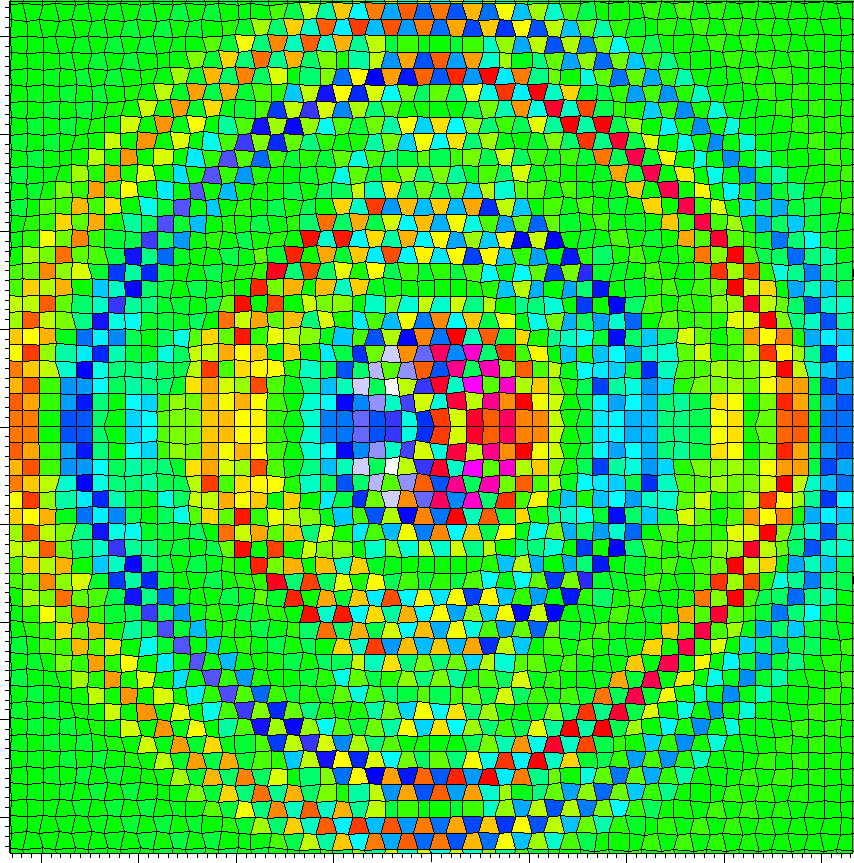
\includegraphics[width=4in,keepaspectratio=true]{./Figures/HGExample.png}
 % gradpField.png: 871x527 pixel, 90dpi, 24.59x14.88 cm, bb=0 0 697 422
 \caption{Example of a “checkerboard” instability in the pressure field and corresponding “hourglass” instability in velocity field; excited by applying a time dependent perturbation to a single node at the center. Instability exists at highest spatial frequency of the underlying grid irrespective
of mesh resolution and is a result of a fundamental instability in the discrete representation of velocity, pressure and the spatial differential operators which relate them.}
 \label{fig:HGExample}
\end{figure}

\begin{figure}[h!]
 \centering
 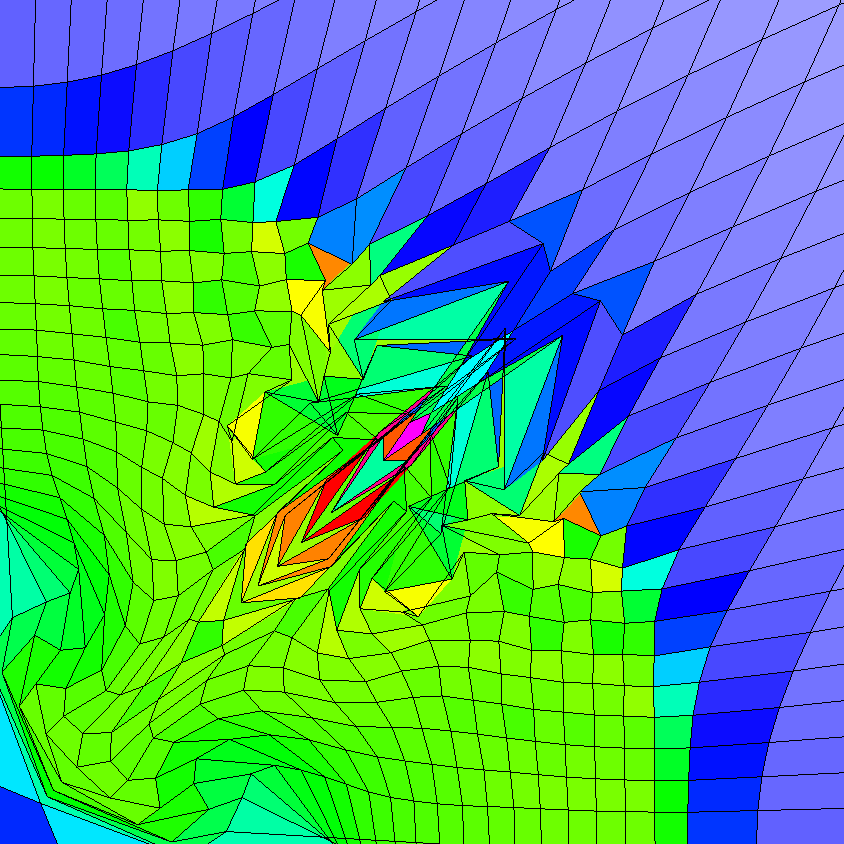
\includegraphics[width=4in,keepaspectratio=true]{./Figures/Noh_SymmetryBreak.png}
 % gradpField.png: 871x527 pixel, 90dpi, 24.59x14.88 cm, bb=0 0 697 422
 \caption{Example of spurious grid distortion encountered when applying standard SGH methods to the Noh problem on an initially orthogonal mesh. There are multiple sources of this grid distortion including hourglass instabilities, inaccuracies in the pressure gradient operator and discretization of the artificial viscosity term. Each of these errors can amplify each other over time, leading to a rapid tangling of the grid.}
 \label{fig:Noh_SymmetryBreak}
\end{figure}

A high order finite element test-bed has been developed in Matlab to evaluate the potential of high order finite elements for Lagrangian hydrodynamics. Several test problems will be considered to assess the usefulness of such methods. A set of static convergence tests will measure and compare the convergence rates of several methods. A significant concern with any new method is the presence of spurious velocity and pressure modes; this will be observed through the acoustic wave problem. The Sod shock tube will evaluate the one-dimensional convergence to the exact solution of a real time-evolving solution, while the Noh problem will bring this evaluation to two dimensions. The Saltzman piston will measure how conducive each method is to propagating a shock wave that is misaligned with the mesh, this will primarily be a test of the artificial viscosity formulation. Finally, the Sedov explosion problem will compare the adaptivity of low and high order methods to curved phenomena. The biggest worry when considering any higher order numerical method is high-frequency ``ringing'' about the shock front. The severity (or not) of this property will be noted as it comes up.

Chapter 2 of this thesis will develop a theoretical framework for arbitrarily high order finite element schemes for Lagrangian hydrodynamics, while Chapter 3 will consider the implementation details in the \texttt{Fermium} code. Chapter 4 narrows the problem domain from a wide range of bi-linear and bi-quadratic elements to four mixed finite element pairs which bear further consideration. Numerical results for each of these methods are presented in Chapter 5 and conclusions are drawn in Chapter 6. % Introduction

% Chapter 2

\chapter{Theoretical Discussion}\label{chap:Theory}
What follows is a review of the theory for arbitrarily high order finite elements for Lagrangian hydrodynamics. Much of this formulation previously appeared in \cite{DobrevEllisKolevRieben2010}.

\section{Euler Equations in a Lagrangian Frame}
The Navier-Stokes equations can be simplified for high Reynolds number flows by assuming that inertial forces are much more significant than viscous forces. Thus all viscous terms can be neglected. This simplified set of four equations are known as the Euler equations and must be solved for four unknowns: velocity $\vec{v}$, density $\rho$, internal energy $e$, and pressure $p$. The Euler equations in a Lagrangian frame are listed below, where $\frac{\mathrm{d}}{\mathrm{d}t}$ represents the total (or advective) derivative. Also please note that these equations are valid for gas dynamics, not the more general case of solid dynamics where scalar pressures would need to be replaced by stress tensors.
\begin{eqnarray}
  \text{Momentum Conservation:}\;\;\;\;\;\; 
  \rho \frac{\mathrm{d} \vec v}{\mathrm{d} t}        &=& 
  - \Grad p                                            
  \label{eq:MomentumConservation}                     \\
  \text{Mass Conservation:}\;\;\;\;\; 
  \frac{1}{\rho}\frac{\mathrm{d} \rho}{\mathrm{d} t} &=& 
  - \Div \vec v                                          
  \label{eq:MassConservation}                         \\
  \text{Energy Conservation:}\;\;\;\;\;\; 
  \rho \frac{\mathrm{d} e}{\mathrm{d} t}             &=& 
  - p \Div \vec v                                                            
  \label{eq:EnergyConservation}                       \\
  \text{Equation of State:}\;\;\;\;\;\;\;\;\;\;\; 
  p                                              &=& 
  EOS(\rho,\; e)                                                          
  \label{eq:EquationOfState}                        
\end{eqnarray}
The Euler equations describe the relationship between fluid motion and the kinematic properties of the fluid such as pressure, energy, and density over a spatial domain $\Omega$. The Equation of State (EOS) describes the relationship between the thermodynamic state variables and provides the necessary closure to the set of equations. In a hydrocode the density and energy of a material are fairly straightforward to calculate each time step. The EOS takes these variables as inputs and allows us to calculate the pressure of the material which is necessary for predicting the future movement of the fluid. The total mass in the spatial domain $\Omega$ is defined to be
\newEq{Mass}{
  m \equiv \int_{\Omega} \rho    
}
Furthermore, the total kinetic energy in the spatial domain 
$\Omega$ is defined as
\newEq{KEDef}{
  KE = \frac{1}{2} \int_{\Omega} {\rho \vec v} \cdot \vec v    
}
The total internal energy in the spatial domain $\Omega$ is defined
as
\newEq{IEDef}{
  IE = \int_{\Omega} \rho e
}
The total energy contained in the spatial domain $\Omega$ is thus
\newEq{TOTEDef}{
  E = KE + IE 
}
If the spatial domain $\Omega$ contains no energy sources (or sinks)
and there is no flux of energy and/or mass out of the boundary of the
domain, $\partial \Omega$, then the total energy contained in 
$\Omega$ is a constant for all time
\newEq{ECons}{
  \frac{\mathrm{d} E}{\mathrm{d} t} = 0
}

\section{A Brief Summary of the Finite Element Method}
The finite element method (FEM) is a powerful numerical technique for solving partial differential equations (PDE) on complicated domains. In contrast to the finite difference method which finds a solution to a finite difference approximation of the differential equation, the FEM finds an approximate solution to the weak form of the original differential equation restricted to a (finite element) subspace. 

\subsection{The Weak Statement of the Problem}\label{sec:WeakStatement}
The first step in the solution to any problem is to first define the problem itself. The FEM requires that the problem be described in a specific format known as the variational or weak statement of the problem \cite{Hughes1987}. Any differential equation can be reformulated to fit into this required format. In brief, you must multiply the differential equation by test function and integrate both sides of the resulting equation over the problem domain. After an integration by parts some of the derivatives are transferred over to the test functions. The resulting system of equations is the variational formulation of the problem. For our purposes, the test functions are chosen to be the same set as the basis functions according to Galerkin's method. We formulate the weak statement of the Euler equations in \refSec{MomentumCons}.

\subsection{Basis Functions}
The approximation to the solution of the differential equation is built up from a set of analyst-selected \emph{basis functions}. The solution to the PDE is assumed to be the summation of all basis functions multiplied with a set of unknown coefficients known as degrees of freedom (DOF). Generally, the basis functions may be any function at all, but typically they are chosen to be piecewise continuous polynomials defined such that they are valued 1 at their own DOF and zero at all others. Thus, when all basis functions are summed up with their respective DOF coefficients, the overall solution will assume values of a DOF at that DOF location and interpolate polynomially to adjacent DOFs. 

As mentioned previously, traditionally staggered grid approaches have associated velocities with vertices and thermodynamic variables have been associated with zone centers and defined as piece-wise constant values. Our general FEM approach treats each field -  $\vec{v}$, $\rho$, $e$, and $p$ as finite element functions on the computational mesh $\tilde\Omega(t)$ with the following expansions
%  for $\vec{x}\in\Omega(t)$

\begin{eqnarray}
  \vec v(\vec x,t) \approx
  \sum_{i}^{N_\mathbf{v}} \mathbf{v}_i(t) \; \vec w_i(\vec x, t) \,,
  \label{eq:DiscreteV} \\
  \rho(\vec x,t)  \approx
  \sum_{i}^{N_\mathbf{r}} \mathbf{r}_i(t) \; \psi_i(\vec x, t) \,, \label{eq:DiscreteRho} \\
  e(\vec x,t)  \approx
  \sum_{i}^{N_\mathbf{e}} \mathbf{e}_i(t) \; \theta_i(\vec x, t) \,, \label{eq:DiscreteE} \\
  p(\vec x,t) \approx
  \sum_{i}^{N_\mathbf{p}} \mathbf{p}_i(t) \; \phi_i(\vec x, t) \,.
  \label{eq:DiscreteP}
\end{eqnarray}

These basis functions will move with the mesh. Furthermore, for simplicity and ease of computation basis functions will be defined on the reference zone and mapped to physical space via the Jacobian of transformation, see \ref{sec:JacobianTransformation}.

\begin{figure}[h!]
 \centering
   \centerline{
    \mbox{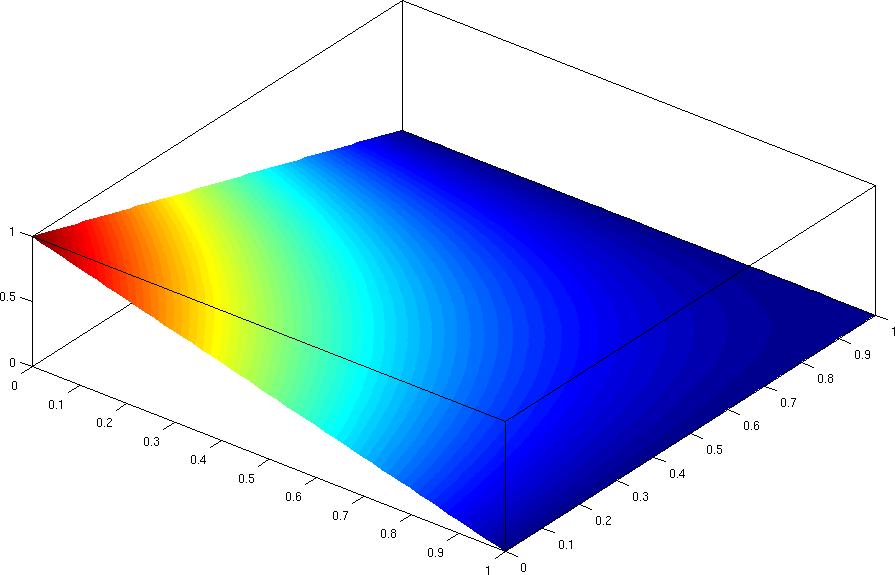
\includegraphics[width=2.00in]{./Figures/Q1Basis.png}}
    \mbox{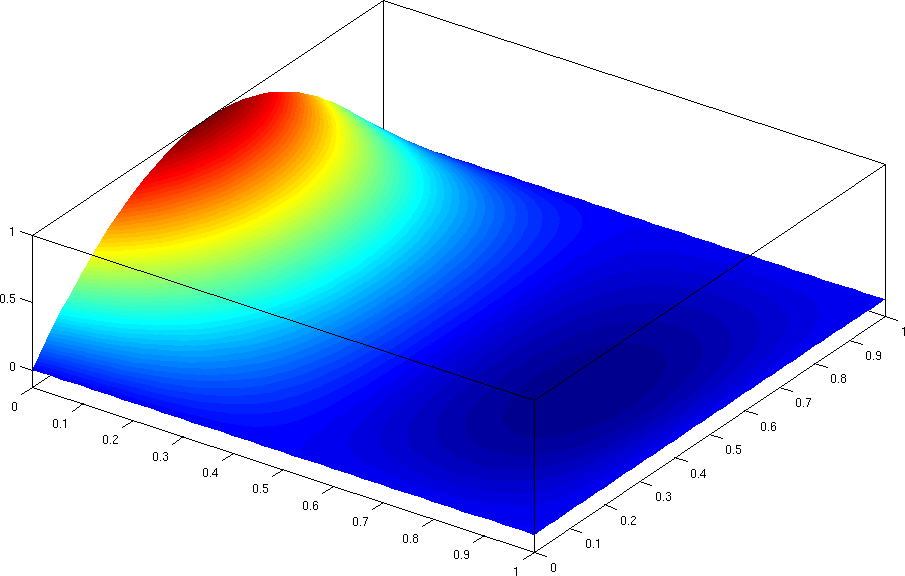
\includegraphics[width=2.00in]{./Figures/Q2Basis.png}}
    \mbox{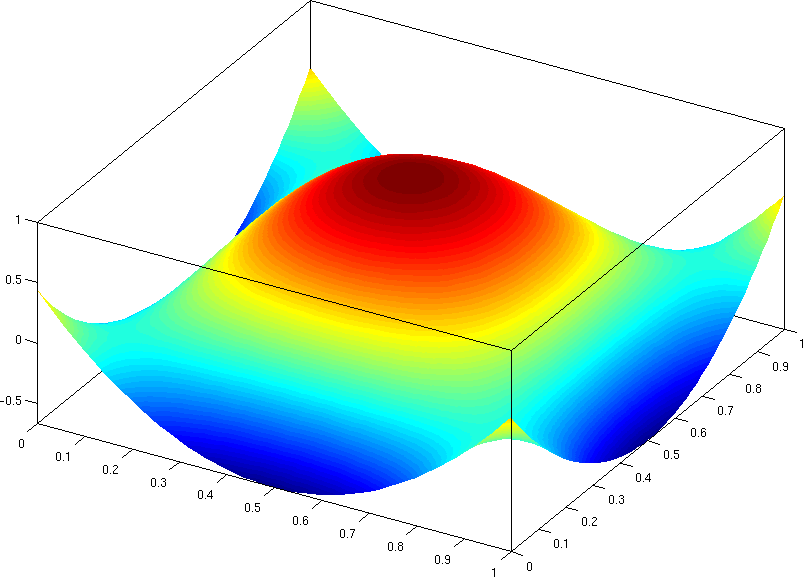
\includegraphics[width=2.00in]{./Figures/Q2dBasis.png}}
  }
 \caption{Examples of 2D basis functions on a reference zone: a standard $Q_1$ bi-linear function that interpolates at nodes \textit{(left)}, a $Q_2$ bi-quadratic function defined at the Gauss-Lobatto quadrature points \textit{(center)} and a $Q_2$ bi-quadratic function defined at the Gauss-Legendre quadrature points \textit{(right)}.}
 \label{fig:ExBasis}
\end{figure}

\section{Mesh}
The basic premise of the Finite Element Method (FEM) is to divide a large complicated problem into a system of smaller simpler problems. In order to do this, we need to divide the problem domain into a number of non-overlapping volumes or zones (aka elements). The governing equations are then solved on each of these smaller domains and assembled to obtain an overall solution to the problem. 

\subsection{Domain Decomposition}
The FEM requires us to take many integrals as we set up the system of simple problems. It is difficult to take an integral over an arbitrary region, especially in an automated fashion. Thus, the first step is to divide the arbitrarily complicated problem domain into a number of simpler zones. In 2-D These zones or elements are usually three- or four-sided but can be more complicated. Each side is defined by a polynomial curve. Traditionally, first order curves, i.e. straight lines are used to connect vertices, but quadratic, cubic, or even higher order curves can be used. \refFig{DomainDecomp} illustrates this process.

\begin{figure}[h!]
\begin{center}
$\begin{array}{c@{\hspace{.35in}}c@{\hspace{.35in}}c}
\includegraphics*[height=2.0in,keepaspectratio=true]{./Figures/DomDecomp1.png}  &  
\raisebox{0.75in}{{\Huge $\mathbf \longrightarrow$}} &
\includegraphics*[height=2.0in,keepaspectratio=true]{./Figures/DomDecomp2.png}   \\
\mbox{\Large $\mathbf{\Omega}(t_0)$} & & \mbox{\Large{$\tilde{\mathbf{\Omega}}(t_0)\equiv \bigcup_z \mathbf{\Omega}_z(t_0)$}} \\
\end{array}$
\end{center}
\caption{Domain decomposition for a finite element mesh}
\label{fig:DomainDecomp}
\end{figure}

Now that we have divided our problem domain into a number of smaller zones, we can link these together to form the \emph{computational mesh}, denoted by $\tilde{\Omega}$ and defined as
\newEq{FEMMesh}{
  \Omega(t_0) \approx \tilde{\Omega}(t_0) \equiv \bigcup_z \Omega_z (t_0)
}
The computational mesh is composed of two sets of information. The \emph{topology}\label{sec:topology} defines the connectivity of the mesh: which nodes belong to which element and which elements share faces, etc. The \emph{geometry} connects nodes to coordinates in physical space. For example, if you wish to compute the volume of element $n$, you must first follow the topology to determine which nodes are connected to element $n$ and the ordering of these nodes. Then you must follow the geometry to find the physical coordinates of these nodes. Once you know the physical locations and ordering of the nodes, then you can perform the desired calculations. 

Curved physical geometries occur frequently in problems of engineering interest. The Sedov explosion problem is a simplified model of an explosive blast propagating through a gas, a problem significant to many fields of engineering. If we take an initially straight Cartesian mesh and continuously apply the exact solution of the Sedov explosion problem to the nodes and edges, we obtain the mesh shown in \refFig{ExactSedovMesh}. The obviously curved elements, especially surrounding the origin motivate the need for zones with curved edges. We would eliminate much of the domain decomposition error if elements had the flexibility to follow curved geometries more closely.

\begin{figure}[h!]
 \centering
 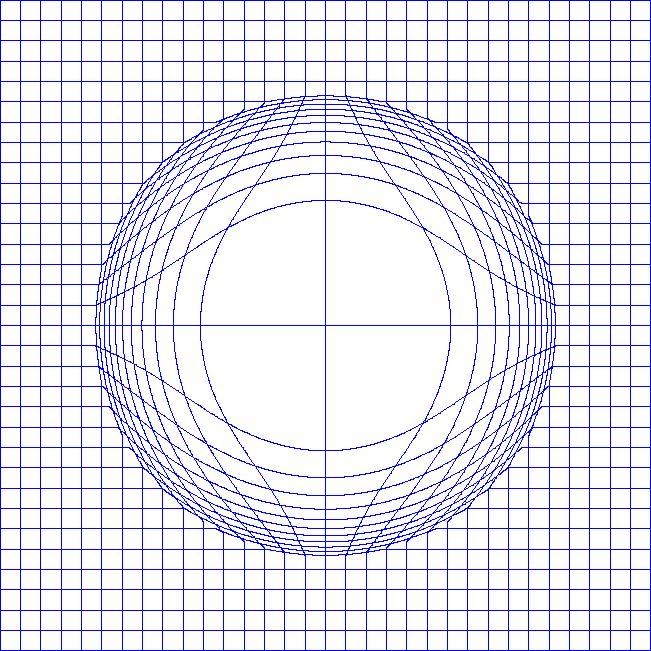
\includegraphics[width=5in,keepaspectratio=true]{./Figures/sedovCart.png}
 % sedovCart.png: 683x683 pixel, 72dpi, 24.09x24.09 cm, bb=0 0 683 683
 \caption{An initial Cartesian mesh is continuously deformed according to the exact solution of the Sedov blast wave.}
 \label{fig:ExactSedovMesh}
\end{figure}

\subsection{Mesh Motion}
By the definition of the Lagrangian framework, for all interesting flows, the computational mesh will move during the process of the simulation. Each element can be thought of as a small volume of fluid that will move and distort in reaction to pressure fields acting on it. We move each volume by tracking a finite number of particles on the boundaries of (and possibly within) that volume known as the \emph{position degrees of freedom}. During each time step, each position degree of freedom is moved according its corresponding velocity degree of freedom and the mesh is reconstructed for the next time step, as illustrated by \refFig{MeshMotion}.

\begin{figure}[h!]
 \centering
   \centerline{
    \mbox{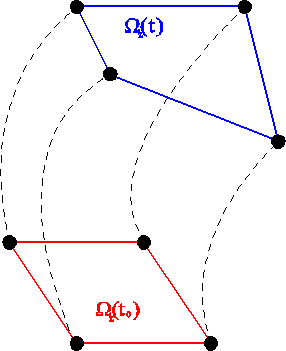
\includegraphics[width=2.00in]{./Figures/motion1.png}}
    \mbox{\hspace*{0.5in}}
    \mbox{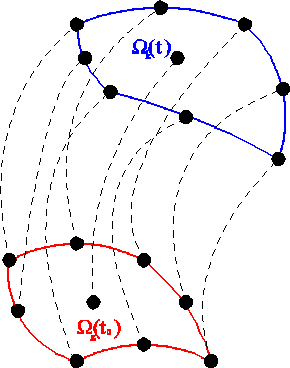
\includegraphics[width=2.00in]{./Figures/motion2.png}}
  }
 % sedovCart.png: 683x683 pixel, 72dpi, 24.09x24.09 cm, bb=0 0 683 683
 \caption{A zone $\Omega_z(t)$ is reconstructed from the evolution of only a few of its points (particles) indicated by black dots. Shown are two specific choices corresponding to the traditional $Q_1$ zone (left) and a high order $Q_2$ zone with curvilinear boundaries (right).}
 \label{fig:MeshMotion}
\end{figure}

\subsection{Jacobian of Transformation}\label{sec:JacobianTransformation}
Even an initially perfectly Cartesian mesh can get rather distorted in the process of a simulation. As mentioned previously, one of the motivations to divide the problem domain into regular zones with regular topology was to ease the process of integration. But integrating over arbitrary distorted zones, especially autonomously, is not a completely trivial matter. This is where the Jacobian of transformation comes in. 

The Jacobian matrix is used as a mapping from a standard reference zone $\tilde{\Omega_z} = [0,1]^2$ to physical space, see \refFig{JacMapping}. We can write the mapping in a functional form as 

\begin{equation}
 \vec{x}=\Phi(\hat{\vec{x}},t), \label{eq:parametricMapping}
\end{equation} 

where $\vec{x}$ denotes a point in physical space and $\hat{\vec{x}}$ denotes the corresponding point in the reference zone. This coordinate transformation is referred to as the parametric mapping and is defined by the physical coordinates of the particles associated with each zone. For the case of a traditional $Q_1$ zone geometry consisting of four vertices connected by straight lines, the parametric mapping is bilinear. This thesis explores some of the befits of high order mappings such as $Q_2$ (bi-quadratic) which produce zones with curvilinear geometry as shown in \refFig{JacMapping}. These parametric mappings are computed for each zone using an interpolating polynomial expansion of the form 

\begin{equation}
 \Phi_z(\hat{\vec{x}},t)=\sum_i \vec{x}_{z,i}(t) \eta_i(\hat{\vec{x}}),
\end{equation}

where $\vec{x}_{z,i}(t)$ denote the physical coordinates of the particles describing the zone $z$ at time $t$, see \refFig{MeshMotion}, and $\eta_i$ is the (high order) nodal basis function associated with particle $i$. The collection of all particle coordinates listed consecutively in a vector array is denoted by $\mathbf{x}(t)$. We define the Jacobian matrix for this mapping as

\begin{equation}
 \mathbf{J}_z=\vec{\nabla}_{\hat{\vec{x}}} \Phi_z \quad\quad \mathrm{or} \quad\quad \left(\mathbf{J}_z\right)_{i,j}=\frac{\partial x_i}{\partial \hat{x}_j} \mathrm{.}
\end{equation}

Note that in general, the Jacobian matrix is a \emph{function} of the reference coordinates $\hat{\vec{x}}$ and therefore varies in a zone. 

For bi-linear elements, the Jacobian is defined according to \refEq{Q1Jacobian}, while bi-quadratic elements use the much more complicated entries in \refEq{Q2Jacobian} to assemble the Jacobian matrix. %Bear in mind that these example Jacobian matrices are for 2-D elements, their 3-D equivalent would be 3$\times$3 matrices. %For the full details of a 

\begin{eqnarray}\label{eq:Q1Jacobian}
\mathbf{J}_z(\hat x,\hat y)=\left[
\begin{array}{cc}
 x_2 - x_1 + \hat y(x_1 + x_3 - x_2 - x_4) & x_4 - x_1 + \hat x(x_1 + x_3 - x_2 - x_4) \\
 y_2 - y_1 + \hat y(y_1 + y_3 - y_2 - y_4) & y_4 - y_1 + \hat x(y_1 + y_3 - y_2 - y_4)
\end{array} \right] \nonumber \\
\end{eqnarray}

\begin{figure}[htbp]
\centering
  \includegraphics*[height=2.0in,keepaspectratio=true]{./Figures/Q2_Element_Ref.png}
  \hspace{8mm}
  \raisebox{0.95in}{{\Huge $\mathbf \longmapsto$}}
  \hspace{8mm}
  \includegraphics*[height=2.0in,keepaspectratio=true]{./Figures/Q2_Element_Phys.png}
  \caption{Example of a $Q_2$ bi-quadratic mapping from a reference zone
          (\emph{left}) to a Lagrangian zone (\emph{right}) defined by
          the locations of the 9 Lagrangian particles
          (black dots).
  \label{fig:JacMapping}}
\end{figure}

\clearpage
\begin{eqnarray}\label{eq:Q2Jacobian}
   J_{1,1}  & = &
         (\hat y - 1)(2\hat y - 1)(4\hat x - 3)x_1  
       + (\hat y- 1)(2\hat y - 1)(4\hat x - 1)x_2 \nonumber \\
   & & + \hat y(2\hat y - 1)(4\hat x - 1)x_3  
       + \hat y(2\hat y- 1)(4\hat x - 3)x_4 \nonumber \\
   & & - 4(\hat y - 1)(2\hat y - 1)(2\hat x - 1)x_5 
       - 4\hat y(\hat y - 1)(4\hat x - 1)x_6 \nonumber \\
   & & - 4\hat y(2\hat y - 1)(2\hat x - 1)x_7 
       - 4\hat y(\hat y - 1)(4\hat x- 3)x_8 \nonumber \\
   & & + 16\hat y(\hat y - 1)(2\hat x - 1)x_9 \nonumber \\
%
   J_{1,2} & = &
         (4\hat y - 3)(\hat x - 1)(2\hat x - 1)x_1 
       + \hat x(4\hat y - 3)(2\hat x - 1)x_2 \nonumber \\
   & & + \hat x(4\hat y - 1)(2\hat x - 1)x_3 
       + (4\hat y - 1)(\hat x - 1)(2\hat x - 1)x_4 \nonumber \\
   & & - 4\hat x(4\hat y - 3)(\hat x -1)x_5 
       - 4\hat x(2\hat y -1)(2\hat x - 1)x_6 \nonumber \\
   & & - 4\hat x(4\hat y - 1)(\hat x - 1)x_7 
       - 4(2\hat y - 1)(\hat x - 1)(2\hat x - 1)x_8 \nonumber \\
   & & + 16\hat x(2\hat y - 1)(\hat x - 1)x_9 \nonumber \\
%
   J_{2,1} & = &
         (\hat y - 1)(2\hat y - 1)(4\hat x - 3)y_1  
       + (\hat y- 1)(2\hat y - 1)(4\hat x - 1)y_2 \nonumber \\
   & & + \hat y(2\hat y - 1)(4\hat x - 1)y_3  
       + \hat y(2\hat y- 1)(4\hat x - 3)y_4 \nonumber \\
   & & - 4(\hat y - 1)(2\hat y - 1)(2\hat x - 1)y_5 
       - 4\hat y(\hat y - 1)(4\hat x - 1)y_6 \nonumber \\
   & & - 4\hat y(2\hat y - 1)(2\hat x - 1)y_7 
       - 4\hat y(\hat y - 1)(4\hat x- 3)y_8 \nonumber \\
   & & + 16\hat y(\hat y - 1)(2\hat x - 1)y_9 \nonumber \\
%
   J_{2,2} & = &
         (4\hat y - 3)(\hat x - 1)(2\hat x - 1)y_1 
       + \hat x(4\hat y - 3)(2\hat x - 1)y_2 \nonumber \\
   & & + \hat x(4\hat y - 1)(2\hat x - 1)y_3 
       + (4\hat y - 1)(\hat x - 1)(2\hat x - 1)y_4 \nonumber \\
   & & - 4\hat x(4\hat y - 3)(\hat x -1)y_5 
       - 4\hat x(2\hat y -1)(2\hat x - 1)y_6 \nonumber \\
   & & - 4\hat x(4\hat y - 1)(\hat x - 1)y_7 
       - 4(2\hat y - 1)(\hat x - 1)(2\hat x - 1)y_8 \nonumber \\
   & & + 16\hat x(2\hat y - 1)(\hat x - 1)y_9 \nonumber \\
\end{eqnarray}

\section{Semi-Discrete FEM Approximation}
In the semi-discrete formulation the problem has been discretized in space, but a specific time discretization has not been selected yet. Time could be discretized in a forward Euler-like scheme, a leap-frog scheme, predictor-corrector, or any other time discretization.

\subsection{Momentum Conservation}\label{sec:MomentumCons}
In order to derive a semi-discrete momentum conservation law, we start with the variational formulation or the weak statement of the problem. Multiply \refEq{MomentumConservation} by a vector valued test function $\vec w'$ and integrate over the spatial domain $\Omega(t)$:

\newEq{MomentumIntegral}{
\int\limits_{\Omega(t)}\left(\rho\frac{\mathrm{d}\vec{v}}{\mathrm{d}t}\right)\cdot \vec w'= -\int\limits_{\Omega(t)}\left(\vec{\nabla}p\right)\cdot \vec w'
}

Now, approximating the spatial domain $\Omega(t)$ with the computational mesh $\tilde \Omega(t)$, integrate the right hand side of \refEq{MomentumIntegral} and apply the divergence theorem:

\newEq{WeakMomentum}{
\int\limits_{\tilde{\Omega}(t)}\left(\rho\frac{\mathrm{d}\vec{v}}{\mathrm{d}t}\right)\cdot \vec w'
= \int\limits_{\tilde{\Omega}(t)}p\left(\vec{\nabla}\cdot\vec w'\right)
- \int\limits_{\partial\tilde{\Omega}(t)}p(\vec w'\cdot\hat{n})
}

where $\hat{n}$ is the outward pointing unit normal vector of the surface $\partial\tilde{\Omega}(t)$.

If we substitute the basis function expansions from (\ref{eq:DiscreteV}) for $\vec{v}$ and (\ref{eq:DiscreteP}) for $p$, and for code simplicity's sake assume boundary conditions that will cause the boundary integral term to vanish (otherwise we would need integrate these boundary terms and apply them as sources to the resulting equation), we arrive at
\newEq{MomentumVar3}{
  \int_{\tilde \Omega (t)}
  (\rho  \sum_i^{N_\mathbf{v}}  \frac{\mathrm{d} \mathbf{v}_i}{\mathrm{d} t} \vec w_i) \cdot \vec w' =
  \int_{\tilde \Omega (t)}
  \sum_i^{N_\mathbf{p}} \; \mathbf{p}_i \phi_i
  (\Div \vec w')  \,.
}
As mentioned in Section \refSec{WeakStatement}, we can apply Galerkin's method and pick the velocity basis functions $\vec{w}_j$ as our test functions $\vec w'$. If we do this we will arrive at the following system of linear ordinary differential equations
\newEq{MomentumVar4}{
  \sum_i^{N_\mathbf{v}}
  \frac{\mathrm{d} \mathbf{v}_i}{\mathrm{d} t}
  \int_{\tilde \Omega (t)}
  \rho (\vec w_i \cdot \vec w_j) =
  \sum_i^{N_\mathbf{p}} \mathbf{p}_i
  \int_{\tilde \Omega (t)}
  \phi_i (\Div \vec w_j)  \,.
}
In matrix form this can be written,
\newEq{GlobalMomentum}{
\boxed{
  \mathbf{M} \frac{\mathrm{d} \mathbf{v} }{\mathrm{d}t }  =
  \mathbf{D}^T \mathbf{p}
}}
where $\mathbf{M}$, $\mathbf{D}$, $\mathbf{v}$, and $\mathbf{p}$ are global matrices or vectors (arrays) that are assembled over the entire computational mesh $\tilde\Omega(t)$ with contributions from DOFs in each individual zone $z$. This is known as the assembly operation and can be written as
\begin{eqnarray*}
  \mathbf{M} = Assemble(\mathbf{M}_z), && \mathbf{D} = Assemble(\mathbf{D}_z), \\
  \mathbf{v} = Assemble(\mathbf{v}_z), && \mathbf{p} = Assemble(\mathbf{p}_z) \,.
\end{eqnarray*}
During this global assembly process the topological (see \ref{sec:topology}) information is used to sum to each degree of freedom information from all zones that it is part of. This is analogous to the idea of ``nodal accumulation'' that is present in traditional SGH codes. Note that the resulting mass matrix $\mathbf{M}$ is global in scope and, in general, requires a full linear solve \label{sec:FullLinearSolve} at each time step to arrive at the desired accelerations. This may sound computationally daunting, but some simplifications can be made to significantly speed up this process such as mass lumping. Mass lumping sums each row of the matrix to it's diagonal, reducing the accuracy while eliminating a full linear solve. In general the mass matrix is very sparse and is has not been a major computational bottleneck in the test problems considered. 

The global mass matrix must be assembled from local mass matrices $\mathbf{M}_z$ calculated for each zone. The local mass matrix can be calculated over a zone $z$
\newEq{MassMat}{
  (\mathbf{M}_z)_{i,j} \equiv  \int_{\Omega_z(t)} \rho (\vec w_i \cdot \vec w_j) \,.
}
By its construction, the mass matrix is symmetric positive definite with dimension $ndof_v \times ndof_v$ where $ndof_v$ is the number of x- or y- velocity degrees of freedom per zone. In theory, $\mathbf{M}_z$ should be $(2 \cdot ndof_v) \times (2 \cdot ndof_v)$ to account for both x- and y- velocity degrees of freedom, but in practice they are identical and a single $ndof_v \times ndof_v$ matrix can be used. For example, a $Q_1$ element has 4 x- and 4 y- velocity degrees of freedom while a $Q_2$ element has 9 x- and 9 y- velocity degrees of freedom. Thus the local mass matrix for a $Q_2$ element would be a $9 \times 9$ matrix. 
The local derivative matrix for zone $z$ is defined as
\newEq{DivMat}{
  (\mathbf{D}_z)_{i,j} \equiv \int_{\Omega_z (t)} \phi_i (\Div \vec w_j) \,.
}
The derivative matrix is a \emph{rectangular} of dimension $ndof_p \times ndof_v$ and acts as a map between the two discrete representations of velocity and pressure. It is a discrete version of the $Div$ operator. The transpose of the derivative matrix is also a discrete version of the $Grad$ operator as seen in (\ref{eq:GlobalMomentum}).

\subsection{Computing FEM Matrices}
As mentioned previously, numerical integration is at the heart of the finite element method. The mass and derivative matrices mentioned above take the brunt of this numerical integration effort. In practice, we compute these integrals by transforming them from each Lagrangian zone $\Omega_z(t)$ to the reference zone $\hat{\Omega}$ through the parametric mapping of (\ref{eq:parametricMapping}). For a general integral over a given Lagrangian zone, this transformation gives
\begin{displaymath}
  \int_{\Omega_z (t)} f = \int_{\hat \Omega _z} (f \circ \Phi) \; |\det \mathbf{J}_z|,
\end{displaymath}
for some integrand f, where ``$\circ$'' denotes composition. Integrals are approximated using quadrature of a user-selected order. This integral over the the Lagrangian zone can therefore be replaced with the following weighted sum
\newEq{ApproxIntegral}{
 \int_{\Omega_z (t)} f
%%  \int_{\hat \Omega _z} (f \circ \Phi) \; |\det \mathbf{J}_z|
 \approx
 \sum_{n=1}^{N_q}
 \alpha_n\;
 \left\{
 (f \circ \Phi) \; |\det \mathbf{J}_z|
 \right\}_{\hat{\vec x} = \hat{\vec q}_n} \,,
}
where $\alpha_n$ are the $N_q$ quadrature weights and $\hat{\vec q}_n$ are
quadrature points inside of the reference zone where the integrand is sampled
at. It is important to realize that depending on the functional form of the integrand and the order of the quadrature rule, numerical quadrature is not always exact. Thus, we have introduced additional, though reasonable, approximation error to the solution of the governing equations. Practically, Gauss-Legendre quadrature is preferred for quadrature on quadrilaterals due to great accuracy for relatively few sample points. 

\subsection{Mass Conservation} \label{sec:densityupdateeq}
By the very nature of the Lagrangian description of fluid dynamics, there is no flux across zone boundaries. Hence, the total amount of mass in a zone is constant for all time. 
\newEq{ZoneMassCons}{
  \frac{\mathrm{d} }{\mathrm{d}t} \int_{\Omega _z(t)} \rho = 0\,.
}
In order to allow for high order density field representations, we need to define high order ``mass moments'' for a given zone using the density basis functions from \refEq{DiscreteRho}:
\newEq{MassMoments}{
 \mathbf{m}_{z,i} \equiv
 \int_{\Omega _z(t)} \rho \psi_i \,.
}
We generalize the case of zonal mass conservation to the high order
mass moments by postulating that
\newEq{MassMomentConst}{
  \frac{\mathrm{d} \mathbf{m}_{z,i} }{\mathrm{d}t} = 0 \,.
}
This choice is motivated by the fact that the same equation holds in the
continuous case. Furthermore, \refEq{MassMomentConst} has the same number of
conditions as the number of unknown densities and in particular it implies
\refEq{ZoneMassCons}.
Note that for the case of a piece-wise constant density approximation
(a single mass moment), we recover the traditional definition of
zonal mass conservation. From our basis function representation of the density field \refEq{DiscreteRho}, it follows that
$$
  \mathbf{m}_{z,i}=\sum_j \mathbf{r}_{z,j}\int_{\Omega_z(t)}\psi_i\psi_j \, .
$$
Written in matrix form, we have 
$$
  \mathbf{m}_z = \mathbf{M}^{\rho}_z \mathbf{r}_z
  \qquad\text{where}\qquad
  (\mathbf{M}^{\rho}_z)_{i,j} \equiv \int_{\Omega _z(t)} \psi_i \psi_j \,.
$$
This yields the semi-discrete mass conservation law
\newEq{SemiDiscreteMass}{
\boxed{
  \frac{\mathrm{d} }{\mathrm{d}t}( \mathbf{M}^{\rho}_z \mathbf{r}_z ) = 0
}
}
The above can be viewed as a generalization of the "sub-zonal mass" concept
introduced in  \cite{CaramanaBurtonShashkov98}; it is a statement that
no mass enters or leaves a given sub-volume of the zone.
If we take the limiting case of this idea and impose mass conservation of the
form
$$
  \frac{\mathrm{d} }{\mathrm{d}t} \int_{\Omega'(t)} \rho = 0 \qquad \mbox {for any} \qquad
\Omega'(t) \subseteq \Omega_z(t) \,,
$$
then we obtain the \emph{strong mass conservation principle}\label{sec:strongmass}
\newEq{StrongMassCons}{
  \rho(t) |\det \mathbf{J}_z(t)| = \rho(t_0) |\det \mathbf{J}_z(t_0)|
}
which is a statement of mass conservation for any point in space (not just in
a variational sense). Note that the density defined by this equation is not
polynomial.

We can write the following relation between the finite element density
function defined by \refEq{SemiDiscreteMass} and the function defined by
\refEq{StrongMassCons} (denoted here by $\rho_h$ and $\rho_s$, respectively)
\newEq{DensityRelation}{
\int_{\Omega_z(t)} \rho_{h} \psi_i = \int_{\Omega_z(t)} \rho_{s} \psi_i
}
which tells us that $\rho_h$ is the projection of $\rho_s$ on the space
spanned by $\{\psi_i\}$.

\subsection{Energy Conservation}
What follows is a general derivation of energy conservation for arbitrarily high order representation. High order energy is still in the experimental stages in \texttt{Fermium}, and all numerical results are presented with piece-wise constant energies. Thus in practice, we use only \refEq{SemiDiscreteEnergyConst}.

If we multiply the energy equation, \refEq{DiscreteE} by a vector valued test function, $\theta_j$ and integrate over a local spatial domain, $\Omega_z(t)$ we arrive at a local formulation for the energy conservation equation
$$
  \int_{\Omega _z(t)} \rho \frac{\mathrm{d} e}{\mathrm{d}t} \theta_j =
  \int_{\Omega _z(t)} p (\Div \vec v) \theta_j\,.
$$
Inserting the basis function expansions for internal energy, pressure and velocity from (\ref{eq:DiscreteV} - \ref{eq:DiscreteP}) we obtain 
\newEq{SemiDiscreteEnergy}{
\boxed{
\mathbf{M}^e_z \frac{\mathrm{d} \mathbf{e}_z}{\mathrm{d}t} =
  - \mathbf{p}_z \cdot \mathbf{D}^e_{z} \cdot \mathbf{v}_z
}
}
where
$$
  (\mathbf{M}^e_z)_{i,j}     \equiv \int_{\Omega _z(t)} \rho \theta_i \theta_j
  \qquad\mbox{and}\qquad
  (\mathbf{D}^e_{z})_{i,j,k} \equiv \int_{\Omega _z(t)} \phi_i \theta_j (\Div \vec w_k) \,.
$$
Here $\mathbf{D}^e_{z}$ is tensor of rank 3 satisfying
$\mathbf{D}_{z} = \mathbf{D}^e_{z} \cdot \mathbf{1}^e_z$, i.e.,
$(\mathbf{D}_{z})_{i,k} = \sum_j (\mathbf{D}^e_{z})_{i,j,k} (\mathbf{1}^e_z)_j$,
where $\mathbf{1}^e_z$ is the zonal representation of the constant $1$ in the
internal energy space (a vector of ones for nodal finite elements).  In this
formulation, the matrix $\mathbf{F}_z = \mathbf{p}_z \cdot \mathbf{D}^e_{z}$ can
be used to generalize the concept of ``corner forces'' (see below), since
$\mathbf{F}_z^T \cdot \mathbf{1}^e_z$ gives the zonal forces in the momentum
equation, while $\mathbf{F}_z \cdot \mathbf{v}_z$ is the work term due to
the pressure gradient forces.

Given the above definitions, we can show that the following semi-discrete energy
conservation relation holds:
\newEq{SemiDiscreteEnergyCons}{
  \frac{\mathrm{d} \tilde E }{\mathrm{d}t} = \frac{\mathrm{d} }{\mathrm{d}t}
  \left(
    \frac{1}{2} \mathbf{v} \cdot \mathbf{M} \cdot \mathbf{v} +
    \sum_z
    \mathbf{1}^e_z \cdot \mathbf{M}^e_z \cdot \mathbf{e}_z
  \right)
  =
  \frac{1}{2} \mathbf{v} \cdot \frac{\mathrm{d} \mathbf{M}}{\mathrm{d}t} \cdot \mathbf{v} +
  \sum_z
  \mathbf{1}^e_z \cdot \frac{\mathrm{d} \mathbf{M}^e_z}{\mathrm{d}t} \cdot \mathbf{e}_z \,,
}
where $\tilde E$ denotes the total discrete energy in the computational
domain. Note that there is both a kinetic energy term and an internal energy
term and that the time rate of change of this sum is equal to zero (implying
total energy conservation) when the time derivatives of the mass matrices
$\mathbf{M}$ and $\mathbf{M}^e_z$ are zero. For the case where the mass matrices change in time (implying a redistribution of mass within a zone), this change must be taken into account in order to maintain exact energy conservation.

Now consider the special case of piece-wise constant internal energies (i.e. a single constant basis function), and denote the (single) zonal mass by $\mathbf{m}_z$. Then, \refEq{SemiDiscreteEnergy} reduces to the form
\newEq{SemiDiscreteEnergyConst}{ \mathbf{m}_z \frac{\mathrm{d} \mathbf{e}_z }{\mathrm{d}t} = -
\mathbf{p}_z \mathbf{D}_z \mathbf{v}_z\;.  }
This can be viewed as a generalization of the so called "compatible hydro" approach of  \cite{CaramanaBurtonShashkov98} by noting that the term $\mathbf{p}_z \mathbf{D}_z$ is simply a collection of "corner forces" due to the discrete pressure gradient term and therefore
$$
  (\mathbf{p}_z \mathbf{D}_z) \mathbf{v}_z = \sum_i \vec f_i \cdot \vec v_i \,.
$$

\subsection{Equation of State}
We can consider the equation of state \refEq{EquationOfState} as either a weak formulation of the equation or simply point by point. As an example, the variational formulation of the gamma-law energy equation $p=(\gamma-1)\rho e$ is
$$
  \int_{\Omega _z(t)} p \phi_j =
  \int_{\Omega _z(t)} (\gamma -1) \rho e \phi_j\,.
$$
This can be written in matrix form (for constant $\gamma$) as
\newEq{EquationOfStateWeak}{
  \boxed{
    \mathbf{M}^{\rho}_z \mathbf{p}_z = (\gamma - 1) \mathbf{M}^{p e}_z \mathbf{e}_z
  }
}
where $\left( M^{pe}_z\right)_{ij} = \int \rho \phi_i \theta_j$.
In \texttt{Fermium} however, we just evaluate it point by point.

\section{Fully-Discrete FEM Approximation}
The fully discrete approximation takes the spatially discretized approximations and applies a time discretization. Any time discretization could be applied, but for the sake of simplicity, and because this research is more concerned with spatial discretization, we consider only the simple case of a forward Euler-like scheme.

\subsection{Momentum Conservation}
If we take the semi-discrete momentum conservation equation, \refEq{GlobalMomentum} and apply the forward Euler time integration scheme, we get
$$
\boxed{
  \mathbf{M}^{n+1} \mathbf{v}^{n+1} = \mathbf{M}^{n} \mathbf{v}^n +
   \Delta t (\mathbf{D}^n)^{T} \mathbf{p}^n
}
$$
If we apply the strong mass conservation principle from \refEq{StrongMassCons}, we can avoid recomputing the mass matrix every cycle because the mass matrix is constant for all time: $\mathbf{M}^n=\mathbf{M}$. This provides significant improvements to the computational efficiency of the algorithm because you only have to assemble the mass matrix at the initial time step, never again. Please note that this property is purely a construct of the Lagrangian framework, and the mass matrix would need to be reconstructed during the mesh relaxation stage of the ALE calculation.
% This could also make the full linear solve mentioned in \refSec{FullLinearSolve} less demanding because the constant mass matrix $\mathbf{M}$ could be decomposed via LU decomposition or a similar technique. 

\subsection{Mass Conservation}
Because the total mass in each zone remains constant over time, and from equation \refEq{SemiDiscreteMass},
we can update density using
\newEq{FullDiscreteDensity}{
  \mathbf{M}^{\rho,n+1}_z \mathbf{r}^{n+1}_z =
  \mathbf{M}^{\rho,n}_z   \mathbf{r}^{n}_z   = \ldots =
  \mathbf{M}^{\rho,0}_z   \mathbf{r}^{0}_z = \mathbf{m}_z^0\,.
}
or,
\newEq{FullDiscreteDensity-General}{
\boxed{
  \mathbf{M}^{\rho,n+1}_z \mathbf{r}^{n+1}_z = \mathbf{m}^0_z
}
}
In other words, we can calculate a local mass matrix every cycle for each zone and do a small ($4 \times 4$) linear solve for density in the $\hat Q_1$ space) linear solve with the original mass of the zone to calculate the new density degrees of freedom. 

\subsection{Energy Conservation}
If we apply the forward Euler scheme to the semi-discrete energy conservation equation, the change in kinetic energy over a time step $\Delta t$ can be calculated from 
$$
  \frac{1}{2} (\mathbf{v}^{n+1})^T \mathbf{M} \mathbf{v}^{n+1} -
  \frac{1}{2} (\mathbf{v}^{n})^T   \mathbf{M}   \mathbf{v}^{n} =
  (\mathbf{v}^{n+\frac{1}{2}})^T   \mathbf{M}(\mathbf{v}^{n+1} - \mathbf{v}^{n}) =
  \Delta t \mathbf{v}^{n+\frac{1}{2}}(\mathbf{D}^n)^T \mathbf{p}^n\,,
$$
where $\mathbf{v}^{n+\frac{1}{2}} \equiv (\mathbf{v}^{n+1} + \mathbf{v}^{n})/2$. So in order to preserve total discrete energy exactly from time step $n$ to $n+1$, we need the energy update to have the form
\newEq{FullDiscreteEconst-General}{
\boxed{
\mathbf{M}^{e,n+1}_z \mathbf{e}^{n+1}_z =
\mathbf{M}^{e,n}_z \mathbf{e}^{n}_z
- \Delta t \mathbf{p}^{n}_z \cdot \mathbf{D}^{e,n}_z \cdot \mathbf{v}^{n+\frac{1}{2}}_z
}
}
which is a discretization of \refEq{SemiDiscreteEnergy}.
For piece-wise constant energies $\mathbf{M}^{e,n}_z$ is just the total mass in zone $z$ at time $n$.

\subsection{Equation of State}
The equation of state discretization does not depend on time at all. Thus, the fully discrete equation of state is just the semi-discrete equation applied at every time step.
$$
\boxed{
\mathbf{M}^{\rho,n+1}_z \mathbf{p}^{n+1}_z =
(\gamma-1) \mathbf{M}^{p e, n+1}_z \mathbf{e}^{n+1}_z
}
$$
For $Q_0$ energy, this simplifies to $\mathbf{p}^{n+1}_z=(\gamma-1)\mathbf{r}^{n+1}_z \mathbf{e}^{n+1}_z$.

\section{Tensor Artificial Viscosity}
One inherent difficulty in solving the Euler equations is that they emit shocks. This can be particularly disturbing in a Lagrangian simulation because the nearly discontinuous nature of shocks can crush a cell to zero or even negative volume. Artificial viscosity has become a popular method for handling shocks in CFD codes. Artificial viscosity smooths a shock over several zones, where physically the shock would have behaved as a discontinuity. Traditionally, this has been a scalar quantity that activates in regions with high gradients \cite{VonNeumannRichtmyer50}, but this method has not performed well in general cases where the shock wave is not aligned with the mesh \cite{KolevRieben09}. 

In order to properly handle shocks that are not aligned with the mesh, we use a tensor artificial viscosity to resist cell compression proportionate with the direction of the shock. Specifically we implemented the general finite element based tensor artificial viscosity formulation of Kolev and Rieben \cite{KolevRieben09}. This formulation is general enough to easily allow for high order velocity field representations. In brief, this approach takes the momentum and energy conservation equations of \refEq{MomentumConservation} and
\refEq{EnergyConservation} and augments them with a generalized viscous force and its corresponding energy term, respectively. 
$$
    \rho \frac{\mathrm{d} \vec v}{\mathrm{d} t} = - \Grad p       + \Div( \mu \Grad \vec v)
$$
$$
    \rho \frac{\mathrm{d} e}{\mathrm{d} t}      = - p \Div \vec v + (\mu \Grad \vec v):(\Grad \vec v)
$$

As usual, we can apply a variational formulation to the momentum equation and use the velocity basis functions to compute local compression-resistive forces for every zone (analogous to corner forces).
\newEq{StiffMat}{
  \mathbf{f}_z = \mathbf{S}_z \mathbf{v}_z\,,
  \qquad\mbox{where}\qquad
  (\mathbf{S}_z)_{i,j} = \int_{{\Omega}_z(t)}
  (\mu_z \Grad \vec w_i) :
  \Grad \vec w_j \,.
}
Note that, similar to the mass matrix, a global stiffness matrix $\mathbf{S}$ is assembled from all of the zonal stiffness matrices, $\mathbf{S} = Assemble(\mathbf{S}_z)$. It is also the same size, $N_v \times N_v$, where $N_v$ is the total number of velocity degrees of freedom in the domain, and it is symmetric positive definite. Also note that in general, the zone based artificial viscosity coefficient $\mu_z$ is a function of space within each zone. Similar to the corner forces, the tensor artificial viscosity forces update the energy equation through a shock/viscosity heating term through an inner product with the zonal velocity.
$$
  \Delta \mathbf{e}_z = \mathbf{v}_z \cdot \mathbf{S}^e_z \cdot \mathbf{v}_z
$$
where 
$$
  (\mathbf{S}^e_z)_{i,j,k} = \int_{{\Omega}_z(t)}
  (\mu_z \Grad \vec w_i) : (\Grad \vec w_k) \theta_j
$$
and $\mathbf{S}_z = \mathbf{S}_z^e \cdot \mathbf{1}_z^e$. In practice we only care about the viscosity coefficient $\mu_z$ at the quadrature points of the integral in \refEq{StiffMat}: $\mu_z$ has both a linear and quadratic diffusion term similar to the form described in  \cite{KolevRieben09}.

\section{Hourglass Filter}
Hourglass filters become necessary to to run several problems to completion. A low order filter has been developed to counter the observed hourglass modes present in \el{Q_1}{Q_0}. A commonly used filter follows \refEq{Q1Q0HGfilter}, where $SW$, $SE$, $NE$, and $NW$ refer to the four vertices of the $Q_1$ quadrilateral and $hgfrac$ is the user adjusted hourglass magnitude. It is important to note that there is no universally acceptable value for $hgfrac$, sometimes it must be large, others it must be small or zero. This limits the usefulness of hourglass filters.
\newEq{Q1Q0HGfilter}{
hgForces=hgfrac\frac{\mathbf{m}_z}{8\Delta t}\left[\begin{array}{c}
                0.25(V_{SE}-V_{NE}+V_{NW}-V_{SW}) \\
		-0.25(V_{SE}-V_{NE}+V_{NW}-V_{SW}) \\
		0.25(V_{SE}-V_{NE}+V_{NW}-V_{SW}) \\
		-0.25(V_{SE}-V_{NE}+V_{NW}-V_{SW})
               \end{array}\right]}

We have not yet derived such an hourglass filter for higher order elements. As a stopgap, we are using an ``hourglass smoother,'' which is accomplished by leaving a fraction of the linear artificial viscosity term (determined by $hgfrac$) on in expansion as well as compression. This acts to smooth all physical or non-physical high frequency velocity behavior. This is acceptable for the test problems considered, but should be addressed before a full hydrocode is pursued.

\section{Fully-Discrete Scheme}
We now have all of the pieces together to assemble a complete general FEM-based Lagrangian CFD scheme. For computational efficiency, we will use the strong mass conservation principle \refEq{StrongMassCons} to avoid recomputing the velocity mass matrix $\mathbf{M}^n = \mathbf{M}$.
%  and the and the energy matrices $\mathbf{M}^{e,n}_z=\mathbf{M}^{e}_z$. 
% We will also explore the benefits of using mass lumping to further expedite the solution process. Mass lumping allows us to avoid solving a full linear system 
A summary of the details of the full, fully-discrete computational scheme is given below.
\begin{eqnarray*}
\mathbf{F}^n &=& \mathbf{p}^n \cdot \mathbf{D}^{e,n}  -
  \mathbf{v}^n \cdot \mathbf{S}^{e,n} 
\\
\mathbf{M} \mathbf{v}^{n+1} &=& \mathbf{M} \mathbf{v}^n +
  \Delta t (\mathbf{F}^n )^T\!\!\cdot \mathbf{1}^e 
\\
\mathbf{M}^{\rho,n+1}_z \mathbf{r}^{n+1}_z &=&
 \mathbf{m}_z^0 
\\
\mathbf{m}_z \mathbf{e}^{n+1}_z &=& \mathbf{m}_z \mathbf{e}^{n}_z
  - \Delta t \mathbf{F}^n_z \cdot \mathbf{v}^{n+\frac{1}{2}}_z 
% \mathbf{M}^{e}_z \mathbf{e}^{n+1}_z &=&
%   \mathbf{M}^{e}_z \mathbf{e}^{n}_z
%   - \Delta t \mathbf{F}^n_z \cdot \mathbf{v}^{n+\frac{1}{2}}_z 
\\
\mathbf{p}^{n+1}_z &=& (\gamma-1)\mathbf{r}^{n+1}_z \mathbf{e}^{n+1}_z
% \mathbf{M}^{\rho,n+1}_z \mathbf{p}^{n+1}_z &=&
%   (\gamma-1) \mathbf{M}^{e}_z \mathbf{e}^{n+1}_z
\end{eqnarray*}
We first calculate local ``corner forces''
% $$
% (\mathbf{F}^n_z)_{i,j} = \int_{\Omega_z(t_n)} \left(
% p^n I - \mu_z^n \Grad \vec v^n \right) : \Grad \vec w_i\, \phi_j
% $$
% $$
% (\mathbf{F}^n_z)_{i,j} = \int_{\Omega_z(t_n)} \left(
% p^n I\right): \Grad \vec w_i\, \phi_j - \left(\mu_z^n \Grad \vec v^n \right) : \Grad \vec w_i\, \theta_j
% $$
$$
(\mathbf{F}^n_z)_{i,j} = \int_{\Omega_z(t_n)} \left(
p^n I - \mu_z^n \Grad \vec v^n \right) : \Grad \vec w_i\, \theta_j
$$
on the current mesh $\Omega^n$ which we assemble into a global force vector $\mathbf{F}^n$. We then use the momentum conservation equation to solve for accelerations and the new velocity degrees of freedom. After moving the mesh from $\Omega^n \mapsto \Omega^{n+1}$, via 
$$
\mathbf{x}^{n+1} =
\mathbf{x}^{n} + \Delta t \mathbf{v}^{n+1} \,,
$$
we can update the new density and energy degrees of freedom. Using the equation of state, we can calculate new pressures and move on to the next time step.  % Theoretical Framework 

% Chapter 3

\chapter{Implementation Details}
\label{Chapter3}
In this chapter we take a walk through the Matlab code to examine various implementation details. \refFig{workflow} diagrams an overview of workflow in \texttt{Fermium} (Finite Element Research Methods Implemented Using Matlab). As this code was developed primarily as a test-bed for various high-order finite element methods on a limited set of test problems, no effort has gone toward making a general interface to set up problems of more practical engineering interest. Also, \texttt{Fermium} was developed in Matlab as an initial prototype for a more powerful and general FEM testbed currently being developed in C++.

In order to facilitate debugging and reduce overhead and CPU time, most of the code functions as one giant script file with few actual function calls. This is done via a useful property of Matlab: the ability to embed scripts in other scripts. This allows us to minimize code redundancy while easing the job of debugging and analysis.

\newpage
\begin{textblock*}{7.5in}(.5in,1in)
\centering
   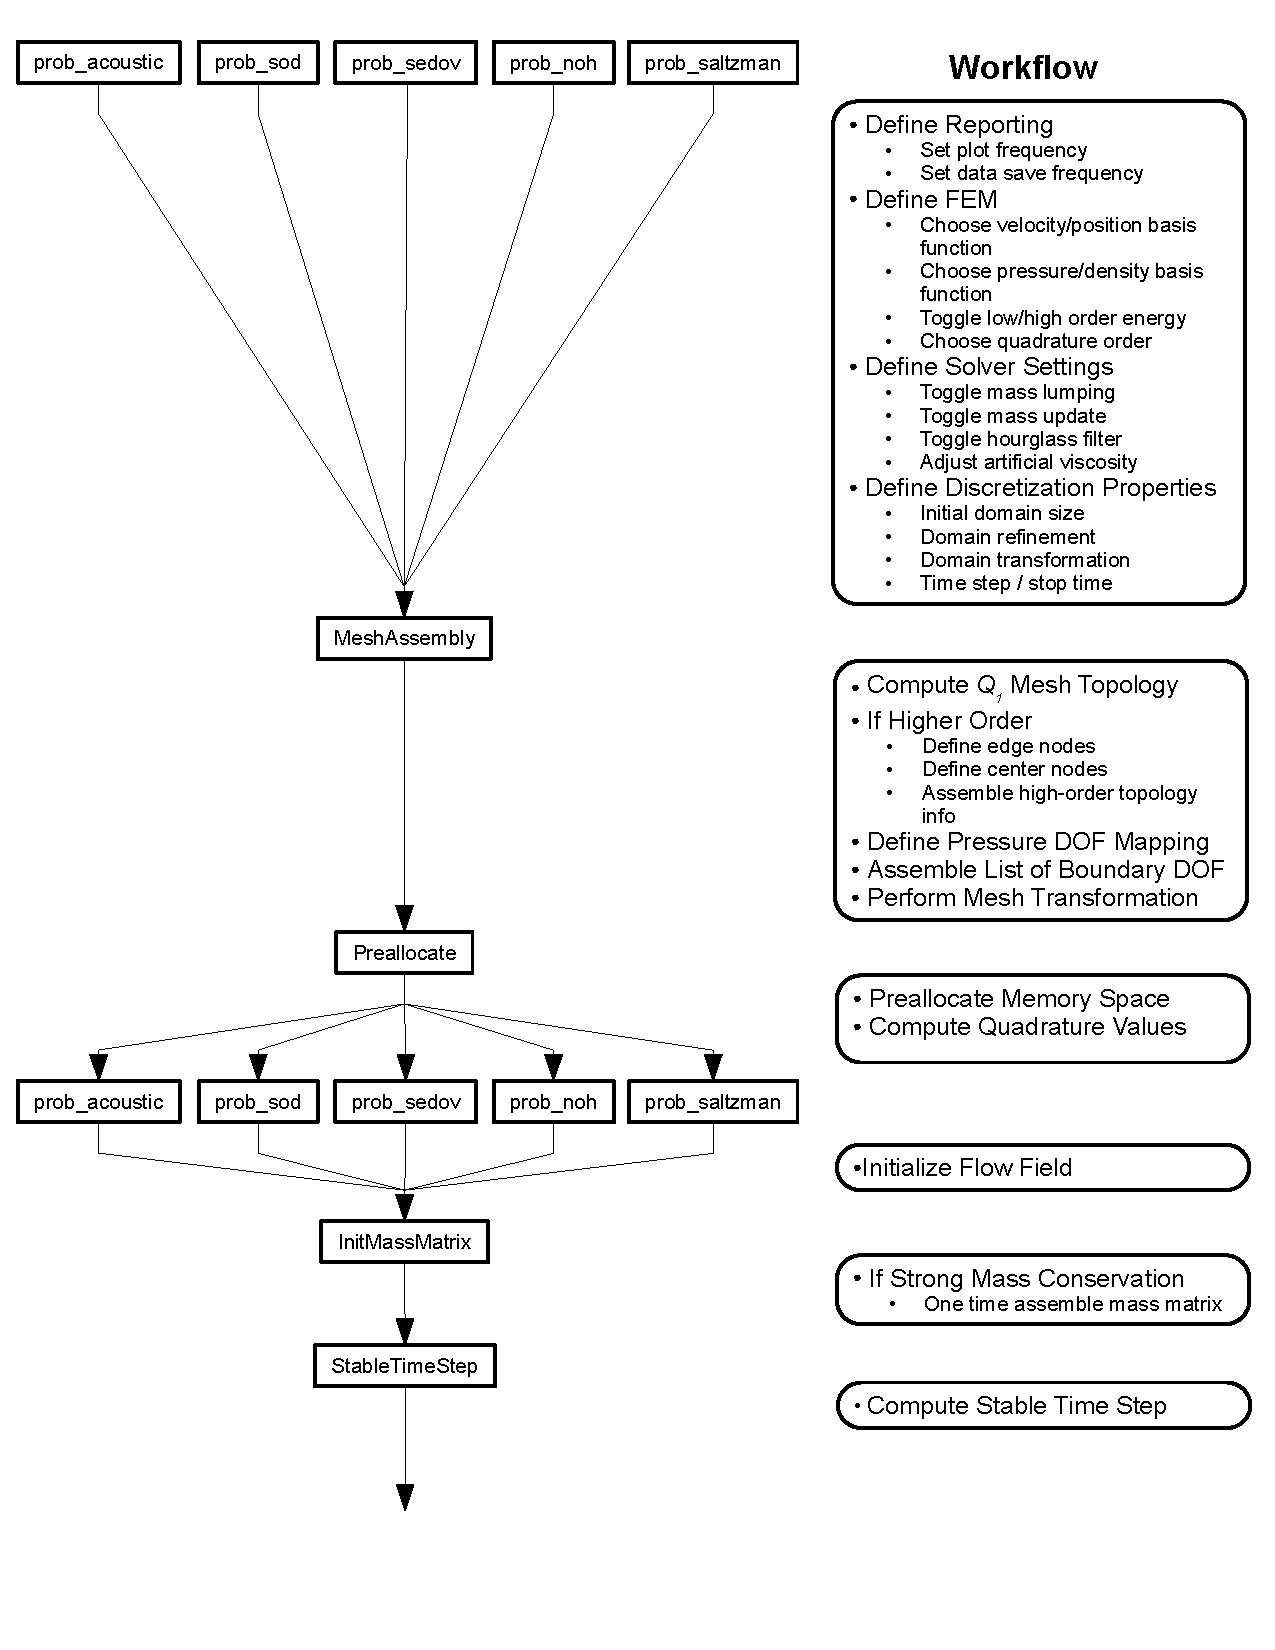
\includegraphics[trim = 0in .5in 0in 0in,clip,width=7.5in,keepaspectratio=true]{./Figures/CodeOutline.pdf}
\end{textblock*}
\mbox{}\clearpage
\newpage

\begin{figure}[p]
\begin{textblock*}{7.5in}(.5in,1in)
\centering
   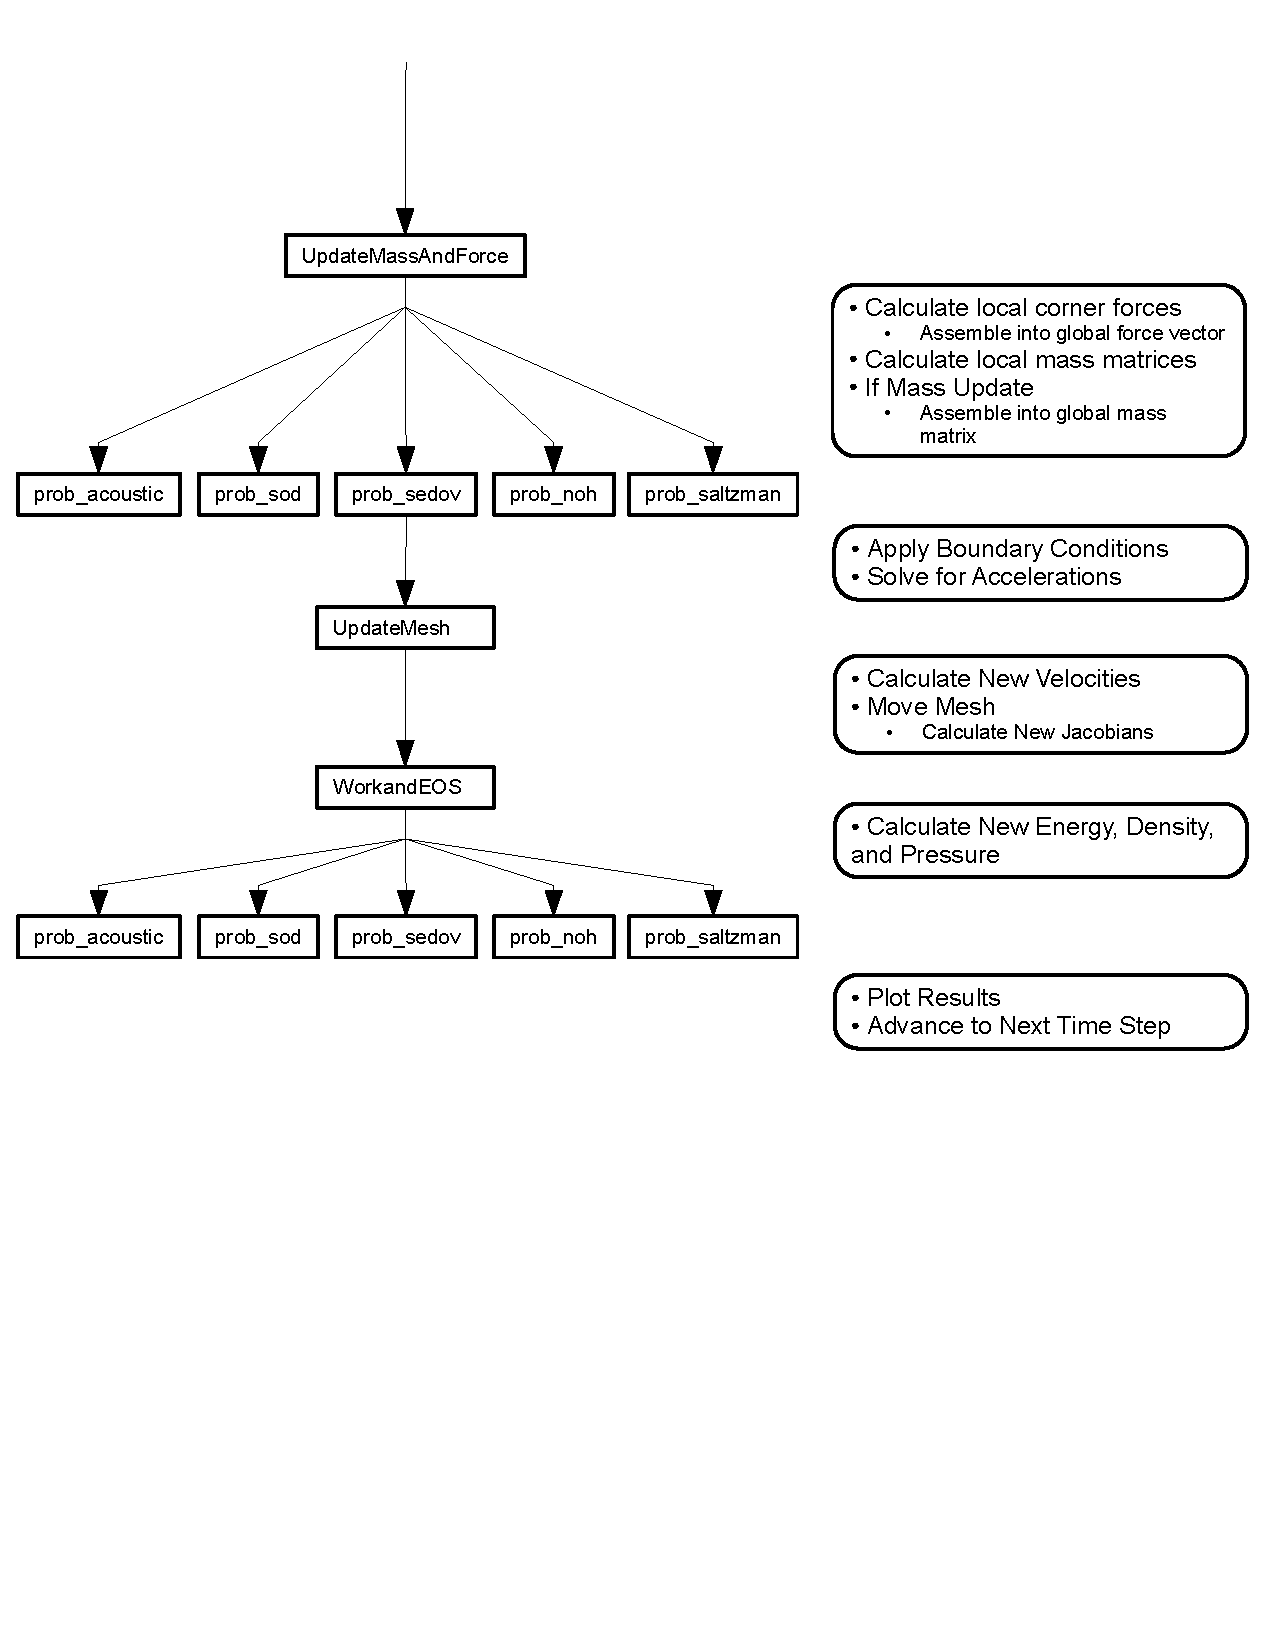
\includegraphics[trim = 0in 4in 0in 0in,clip,width=7.5in]{./Figures/CodeOutline2.pdf}
\end{textblock*}
\begin{textblock*}{3.5in}(2.5in,8in)
\caption{Workflow diagram}
 \label{fig:workflow}
\end{textblock*}
\end{figure}
\mbox{}\clearpage
\newpage

\section{The Drivers} \label{sec:strongmassupdate}
Starting at the top of the workflow diagram, we see the drivers: scripts which define a problem and connect all of the pieces necessary to solve it. We have implemented several classic test problems as drivers including the acoustic wave problem, the Sod shock tube, the Sedov explosion, the Noh implosion, the piston driven shock, and the Saltzman piston, the details of which can be found in \refChap{Elements} (acoustic wave) and \refChap{NumericalResults} (Sod, Noh, Saltzman, and Sedov).

The first thing that we need to set in our code is the method that we want to use to solve the problem. \texttt{Fermium} is general enough to allow for the kinematic and thermodynamic basis functions to be chosen independently. Hence, we have the following options available for the velocity/position basis functions: bi-linear, bi-quadratic, and bi-linear with bubble, as illustrated in \refFig{VelBasisFunctions}. All of these basis functions are defined on quadrilaterals, but there is nothing to prevent us from trying triangles or any other shape (other than the added complexity of going to unstructured grids). We have many more thermodynamic basis functions at our disposal, as depicted in \refFig{PresBasisFunctions}. At this point higher order energy is still in an experimental stage. From some initial results, it looks like we are able to achieve higher order pressure and density behavior while maintaining piecewise constant energy representations. Therefore, although we maintain a switch to use a higher-order energy representation, we usually represent energy as a $Q_0$ field.

\begin{figure}[p!]
 \centering
 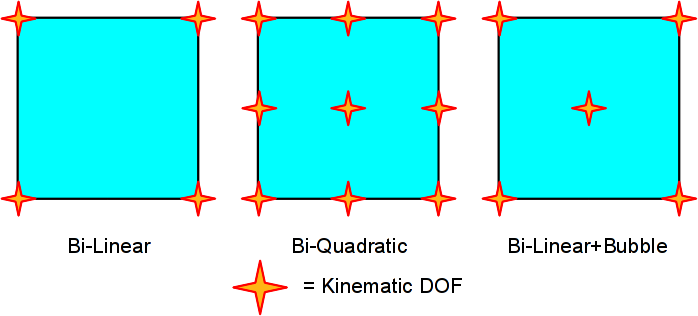
\includegraphics[width=6in,keepaspectratio=true]{./Figures/VelBasisFunctions.png}
 % VelBasisFunctions.png: 698x343 pixel, 107dpi, 16.56x8.14 cm, bb=
 \caption{Options for kinematic basis functions}
 \label{fig:VelBasisFunctions}
\end{figure}

\begin{figure}[p!]
 \centering
 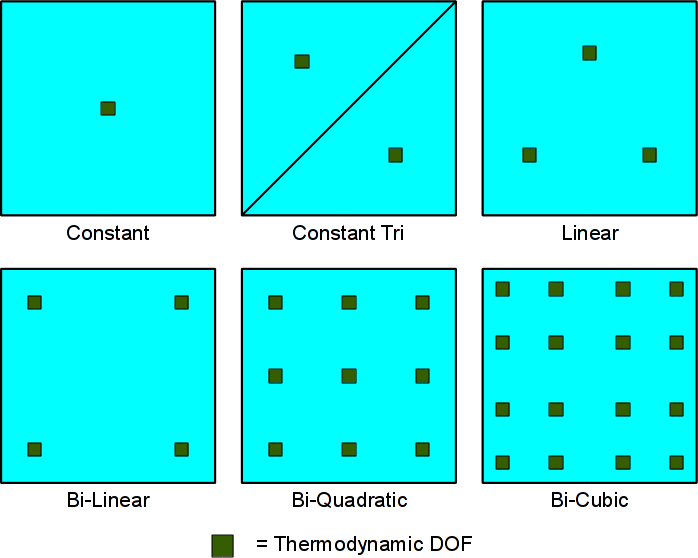
\includegraphics[width=5in,keepaspectratio=true]{./Figures/PresBasisFunctions.png}
 % VelBasisFunctions.png: 698x343 pixel, 107dpi, 16.56x8.14 cm, bb=
 \caption{Options for thermodynamic basis functions}
 \label{fig:PresBasisFunctions}
\end{figure}

Furthermore, the driver has variables to toggle several other solver options. We have derived the concept of \emph{strong mass conservation} (see \refSec{strongmass}), which allows us to avoid recomputing the mass matrix every cycle. The driver script has a switch called \texttt{MassUpdate} that allows us to forgo recalculating our mass matrix every cycle. Another consequence of strong mass conservation is that $\rho |J|=const$. Therefore, if we use $\rho |J|$ as our finite element expansion rather than $\rho$, we don't have to do a density update. The \texttt{StrongMass} switch changes the thermodynamic variables to this representation. This is also somewhat in the experimental stage, so we will mostly consider traditional finite element spaces in this research. There are also knobs to turn on and control hourglass filters and artificial viscosity. In addition to all of this, we use the driver to set the Gauss-Legendre quadrature order and the initial and maximum time steps. The mesh geometry and refinement are also controlled in the header of the driver script. We can also set plot and save-file frequency. \refTab{switches} lists the various parameters and variables that are available in the header along with a few typically used values.

\begin{table}
\centering
  \caption{List of parameters and variables}
  \label{tab:switches}
  \begin{tabular}{|l|p{2.5in}|c|}
  \hline
  Switch or Knob & Possible Values & Typical Value\\
  \hline
  \textsf{recover} & false, path to recover file &\\
  \textsf{SaveFigures} & true, false &\\
  \textsf{nplots} & $\mathbb{N} \in [0,1,2,...)$ & 20\\
  \textsf{nsaves} & $\mathbb{N} \in [0,1,2,...)$ & 10\\
  \textsf{dtInit} & $\mathbb{R} \in (0,\infty)$  & 1e-3\\
  \textsf{dtMax} &  $\mathbb{R} \in (0,\infty)$  & 1e-2\\
  \textsf{maxcycle} &  $\mathbb{N} \in [1,2,...)$ & 1e5\\
  \textsf{VBasis} & \textsf{@Q1Basis, @Q2Basis, @Q1bBasis...} & \\
  \textsf{PBasis} & \textsf{@Q0Basis, @P1Basis, @Q1dBasis...} & \\
  \textsf{HighOrderEnergy} & true, false &\\
  \textsf{StrongMass} & true, false &\\
  \textsf{FullMassMatrixSolve} & true, false &\\
  \textsf{MassUpdate} & true, false &\\
  \textsf{QuadOrder} & $\mathbb{N} \in [1,2,...)$ &\\
  \textsf{hgfrac} &  $\mathbb{R} \in [0,\infty)$ & 1 \\
  \textsf{Qfrac} &  $\mathbb{R} \in [0,\infty)$ & 1 \\
  \textsf{qquad} & $\mathbb{R} \in [0,\infty)$ & 1 \\
  \textsf{qlin} & $\mathbb{R} \in [0,\infty)$ & 1 \\
  \hline
  \end{tabular}
\end{table}

\section{Mesh Assembly and Variable Preallocation}
In the interests of code re-use, we have moved as much functionality as possible to the common files like \textsf{MeshAssembly.m} and \textsf{Preallocate.m}. The \textsf{MeshAssembly} script fleshes out the details of the FEM chosen: defining the number of spatial and thermodynamic DOFs per zone and their location within the reference element. We also need to generate a mesh and define the connectivity of the elements. The function \textsf{ComputeReferenceMeshNodes} creates a Cartesian mesh, $\mathtt{xmin} < x < \mathtt{xmax}$ by $\mathtt{ymin} < y < \mathtt{ymax}$, while \textsf{ComputeMeshTopology} defines the connectivity: which nodes belong to which quad. If the spatial discretization is higher order, we go on to further refine the mesh. If the element has additional edge nodes we place these and, along with the corner connectivity, add the edge connectivity information to \texttt{Quadmap}. Additionally, if the element has center nodes, we add this information to the end of \texttt{Quadmap}. Therefore, the velocity nodes within each element are numbered according to \refFig{VelNodeNumbering} with the corner nodes listed first and center nodes listed last. For data structure reasons, we have formulated each column of \texttt{Quadmap} as an element and each row as a spatial DOF connected to that element.

\begin{figure}[h!]
 \centering
 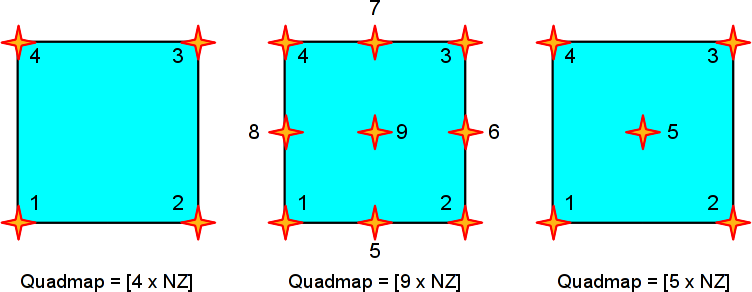
\includegraphics[width=6in,keepaspectratio=true]{./Figures/VelNodeNumbering.png}
 % VelBasisFunctions.png: 698x343 pixel, 107dpi, 16.56x8.14 cm, bb=
 \caption{Velocity node numbering}
 \label{fig:VelNodeNumbering}
\end{figure}

The pressure map is a lot simpler to set up because there is no sharing of DOFs between elements. The \texttt{PressureMap} array is as simple as \refEq{PresMap}, where each column refers to a different element and each row is a different pressure DOF belonging to that element

\newEq{PresMap}{
\mathtt{PressureMap}=\left[
\begin{array}{ccccc}
1 & npdof+1 & 2 \cdot npdof+1 & \cdots & (NZ-1)\cdot npdof+1 \\
2 & npdof+2 & 2 \cdot npdof+2 & \cdots & (NZ-1)\cdot npdof+2 \\
\vdots & \vdots & \vdots & \ddots & \vdots \\
npdof & 2 \cdot npdof & 3\cdot npdof & \cdots & NZ\cdot npdof
\end{array}\right]}

The next step is to determine which DOFs are on which boundary. This is done with the \texttt{ComputeBoundaryDOFQuad} function. \texttt{MeshAssembly} also performs any grid transformation called for by the driver, including randomly distorting the mesh, applying the Saltzman mesh pattern, rotating, or refining the mesh.

The \texttt{Preallocate} m-file mostly just preallocates empty matrices and vectors for speed (as suggested by Matlab). It also evaluates the basis functions, their derivatives, and the Jacobian at the preset quadrature points.

\section{Initializing the Flow Field}
\texttt{Preallocate.m} then returns control back to the driver where the flow field is initialized. Here the initial velocity profile and state variables are specified. After this, the \texttt{InitMassMatrix} script is called. If we are using strong mass conservation to avoid recalculating the mass matrix every cycle, this script assembles the global mass matrix which will be used for every subsequent time step. Once this is done, we go into the time stepping loop.

\section{Solving the Momentum Equation}
The first thing that we need to do at each step is to calculate a stable time increment using the \texttt{StableTimeStep} script. For traditional SGH with an explicit time-marching scheme, this typically involves the Courant–Friedrichs–Lewy \cite{CourantFriedrichsLewy28} condition. We want the time step to be such that a wave will not propagate more than the length of one cell within one time step. This can be written
\[
 \Delta t < C \frac{h}{V}
\]
where $h$ is a measure of the length across a zone, $V$ is the maximum velocity in the zone, and $C$ is typically $1/2$. For higher order elements, we must take sub-zonal physics into account. We define $h$ to be the minimum distance between any two velocity DOFs, $V$ to be the maximum velocity, and $C$ to be $1/4$, just to be safe. 
% This may be overly harsh, but it ensures a stable solution until a more detailed analysis can be performed. 
% We have not yet been able to perform a full stability analysis of high-order curvilinear finite elements, so we have chosen a very strict definition of a stable time step. 

Once we have calculated a stable time step, we dive into the \texttt{UpdateMassAndForce} script file. This script uses the current state of the pressure, velocity, and mesh to calculate forces exerted on each spatial DOF as well as the updated mass matrix (if \textsf{MassUpdate} is turned on). Let's assume for a minute that we are calculating both. To do this, we cycle through every element in the mesh and calculate a local mass matrix and `corner' force using either the \texttt{elemQ1} or \texttt{elemQ2} (this actually works for any higher order velocity basis) function. Hourglass filtering is the only real difference between these two functions. We are still using a very primitive form of an hourglass filter for higher-order elements, so we are handling the $Q_1$ elements, with their well-developed hourglass functions separately. The current $Q_2$ ``hourglass filter'' is not really an hourglass filter, per se. Instead we use a fraction of the linear term of the artificial viscosity. This serves to smooth out high frequency velocity modes, be they physical or not. This is not an acceptable course for a full hydrocode, but we are developing appropriate high order filters. The first step in the \texttt{elem*} functions is to calculate a local mass matrix from the spatial degrees of freedom. After this, we build up the corner forces with contributions from pressure gradients, artificial viscosity, and hourglass forces as described in \refChap{Theory}. 

Once these corner forces and local mass matrices are assembled into the global system via the connectivity information, control is returned to the driver where the boundary conditions are applied and the global systems $\mathbf{M}\vec{a}_x=\vec{F}_x$ and $\mathbf{M}\vec{a}_y=\vec{F}_y$ are solved for the accelerations. This can be done via mass lumping, which accumulates all off-diagonal information to the diagonal of the matrix or a full mass matrix solve. 
% If we are using strong mass conservation and the initial mesh is Cartesian, the full mass matrix will already be diagonal for every time step, which will be the case for all most test cases that we will consider. 

\section{Mesh Movement and Thermodynamic \mbox{Update}}
Once the nodal accelerations have been solved for, the driver gives control to the \texttt{UpdateMesh} common script. This script first accelerates the velocity DOFs according to \refEq{velUpdate}, then it applies any source terms to the velocity before moving the mesh nodes according to \refEq{meshUpdate}.
\newEq{velUpdate}{
\mathsf{NEWvelocity=OLDvelocity+dt*acceleration}
}
\newEq{meshUpdate}{
\mathsf{allnodes=allnodes+dt*NEWvelocity}
}
\texttt{UpdateMesh} then calculates the new Jacobian matrix for every element at every quadrature point for use in the next time step. Finally, it checks for any points where the determinant of the Jacobian is zero or negative, which would indicate that the solution has gone unstable.

Now that we have a new mesh geometry, we can calculate the new thermodynamic properties on this updated mesh using \texttt{WorkandEOS}. Please note that the thermodynamic properties are discontinuous between zones, this allows us to loop over ever element and calculate the new state independent of all other zones without assembling any sort of global system. Thus for each zone, we first calculate the change in internal energy with the dot product of the velocity DOFs and corner forces. We then proceed to the density update. As mentioned previously in \refSec{strongmassupdate}, if we use the basis functions to represent $\rho |J|$ rather than just $\rho$, this function is constant and no density update is required. However, if we are using a traditional representation of density, then we need to compute new density DOFs. The first step is analogous to assembling a local mass matrix, but instead of using the spatial basis functions, we use the density basis functions. We then solve a small $\mathtt{npdof} \times \mathtt{npdof}$ system of equations for the new density degrees of freedom as explained in \refSec{densityupdateeq}. Now that we have the energy and density, we can update the pressure point-wise according to the equation of state.

\section{Plotting}
Finally, now that all variables have been updated for the next time step, we can move back to the driver for the plotting stage. We first check that this is one of the desired plot or save time steps. We have developed several finite element specific plotting routines such as \texttt{PlotFEMContourf} and \texttt{PlotFEMMesh} to accurately represent any arbitrary basis function to any user-specified precision. The driver plots the fields as called for, saves the figures / variable data if requested, then loops back to \texttt{StableTimeStep} for the next time step. This whole process repeats until \textsf{tstop} is reached or \texttt{WorkandEOS} detects that the solution has gone unstable. % Implementation Details

% Chapter 4

\chapter{Some Elements Considered}
\label{chap:Elements}
We have derived a general finite element scheme for Lagrangian computational fluid dynamics. This general framework has made it very easy to consider a number of different mixed finite element formulations. We have only considered quadrilateral 2-D elements in this research, but the formulation is general enough to allow for triangles or even 3-D tetrahedral or hexahedral meshes. In this chapter, we analyze a wide range of bi-linear and bi-quadratic mixed finite element pairs and narrow the results down to four elements to warrant further numerical consideration. Please note that all methods use a $Q_0$ energy representation.

\section{Some Guidelines}
In his canonical textbook on the finite element method, Hughes \cite{Hughes1987} describes some requirements for stable mixed finite element pairs for Stokes flow. The most comprehensive measure of stability is the so-called Ladysenskaja-Babuska-Brezzi (LBB) stability condition. This analysis is far from trivial and several easier estimates of stability have been derived. To our knowledge, no detailed analysis of the LBB condition for Euler's equations has been published. Thus, we used Stokes flow analysis (which has been very thorough), to guide our initial steps in looking for stable basis function pairs. 

Constraint counting is a simpler heuristic approach for determining the suitability of a basis function pair for simulating incompressible Stokes flow. In short, this is the ratio of global kinematic to thermodynamic DOFs after boundary conditions have been applied:
\[
 r=\frac{N_v}{N_p}
\]
where $N_v$ is the total number of velocity degrees of freedom and $N_p$ is the total number of pressure or density degrees of freedom. The ideal value of $r$ is the number of spatial dimensions, $nD$, in the problem (i.e. 2 for two dimensions, 3 for three). A value of less than $nD$ would indicate a tendency of the elements to lock and a larger value would predict poorly approximated incompressibility conditions. Thus, in two dimensions a traditional \el{Q_1}{Q_0} element would have the ideal ratio of 2. We have not yet determined if or how this approach translates to the Euler equations, but it informed our early choices and it appears that pairs that do not satisfy this condition have similar failings.

\section{Convergence Tests}
The most important characteristic of a basis function pair is that it is able to converge to the correct solution under refinement. We have developed two simple static problems to test the accuracy and convergence for the two biggest parts of the momentum equation. The $\mathrm{grad}(p)$ problem tests convergence to the exact solution to the pressure gradient in the momentum equation, while the $\mathrm{div}(\mathrm{grad}(V))$ problem tests the discrete representation of the $\mathrm{div}(\mathrm{grad}())$ operator in the artificial viscosity representation.

\subsection{\texorpdfstring{The $\mathrm{grad}(p)$ Test}{The grad(p) Test}}
Before progressing to further study, it is essential to test whether a specified mixed finite element pair can solve the simplest of problems. With this in mind, we devised a static pressure gradient test to see whether each method could accurately predict nodal accelerations for a specified pressure field. So the pressure field $p=\cos(\frac{\pi}{2}x)\cos(\frac{\pi}{2}y)$, shown in \refFig{gradpField}, is mapped onto two series of meshes on $x,y \in [-1,1]$, one perfectly Cartesian and one distorted, \refFig{randomRefined} . The convergence rate is found by calculating the $L^2$ error norm on these two sets of grids. We first calculate the error due to the projection of an exact pressure field onto its basis function representation, then we calculate the error of the static momentum solve. 

\begin{figure}[h!]
 \centering
 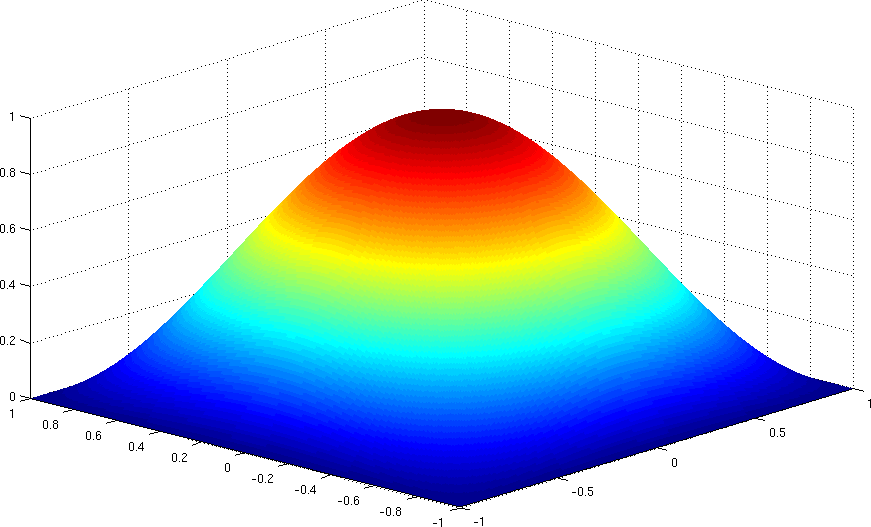
\includegraphics[width=5in,keepaspectratio=true]{./Figures/gradpField.png}
 % gradpField.png: 871x527 pixel, 90dpi, 24.59x14.88 cm, bb=0 0 697 422
 \caption{Initial pressure field}
 \label{fig:gradpField}
\end{figure}

This pressure field was chosen because $p$ is zero on all boundaries (thus eliminating the surface integral in the finite element formulation), and there is a simple analytical expression for the exact accelerations, 
$a=\left[ \begin{array}{c}
           \frac{\pi}{2}\sin(\frac{\pi}{2}x)\cos(\frac{\pi}{2}y)  \\
	    \frac{\pi}{2}\cos(\frac{\pi}{2}x)\sin(\frac{\pi}{2}y)
          \end{array}
 \right]$.

\begin{figure}[h!]
\begin{center}
$\begin{array}{c@{\hspace{.1in}}c@{\hspace{.1in}}c}
\includegraphics*[width=1.8in,keepaspectratio=true]{./Figures/gradpmesh1.png}  &  
\includegraphics*[width=1.8in,keepaspectratio=true]{./Figures/gradpmesh2.png}  &
\includegraphics*[width=1.8in,keepaspectratio=true]{./Figures/gradpmesh3.png}   \\
\end{array}$
\end{center}
\caption{Series of refined distorted meshes}
\label{fig:randomRefined}
\end{figure}

\subsection{The $\mathrm{div}(\mathrm{grad}(V))$ Test}
The $\mathrm{div}(\mathrm{grad}(V))$ test was devised to measure the accuracy and convergence rates of the several methods in approximating the $\mathrm{div}(\mathrm{grad}())$ operator, a calculation that is imperative for the tensor artificial viscosity term in shock problems. In this problem, we project a velocity field,
\[
 \begin{array}{c}
   V_x = \cos(\pi x) \cos(3 \pi y) \\
   V_y = \cos(3 \pi x) \cos(\pi y)
 \end{array}
\]
onto the mesh, $x,y \in [0,1]$. This velocity field is looks like \refFig{divgradV}. We use the same sequence of Cartesian and distorted meshes to establish convergence rates. The first measure of a method is that projection of the velocity field onto the velocity basis functions converges to the exact field under refinement. Finally, we check that the predicted accelerations due to the artificial viscosity converge to the analytically predicted value, \refEq{gradPExactA}.
\newEq{gradPExactA}{
  \begin{array}{c}
   a_x = -\pi^2 \cos(\pi x) \cos(3\pi y)+9\pi^2 \cos(\pi x) \cos(3\pi y) \\
   a_y = -9\pi^2 \cos(3\pi x) \cos(\pi y)+\pi^2 \cos(3\pi x) \cos(\pi y) \\
 \end{array} 
}
This velocity field was chosen for simplicity's sake in order to eliminate the boundary terms in the weak form description. These boundary terms vanish to zero if $\Grad V \cdot \vec{n} = 0$, where $\vec{n}$ is the outward facing unit normal vector of the domain. A simple analysis will confirm that this vector field does indeed satisfy this requirement for this particular domain. We also chose this vector field because it is complicated enough to run our method through the ringer. We have regions of converging, diverging, and swirling flow. Our stiffness matrix needs to be able to capture the details of some complicated flow fields.

\begin{figure}[h!]
 \centering
 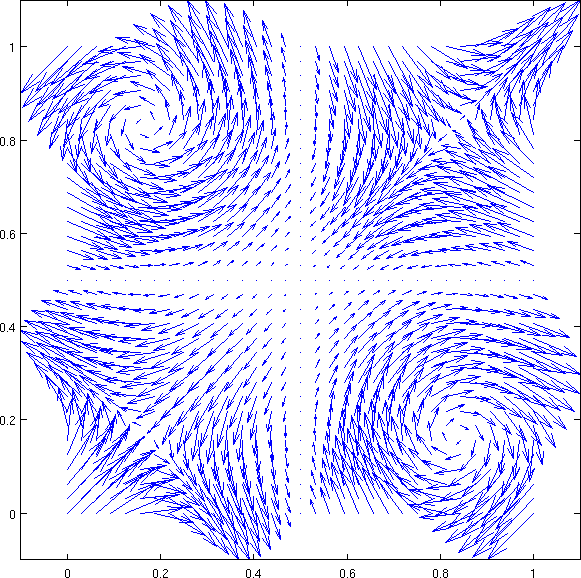
\includegraphics[width=5in]{./Figures/divgradV3.png}
 % gradpField.png: 871x527 pixel, 90dpi, 24.59x14.88 cm, bb=0 0 697 422
 \caption{Projected velocity vector field}
 \label{fig:divgradV}
\end{figure}

\section{The Acoustic Wave Test}
We discovered that a delta function disturbance is the surest way of exciting hourglass modes. In light of this, Robert Rieben developed the acoustic wave test problem to reveal whether a mixed finite element pair exhibits tendencies for hourglass mode instabilities. In this test, a single node in an initially Cartesian mesh is oscillated in time with a small amplitude. Because this is supposed to be a smooth problem and no shocks should show up, all artificial viscosity is turned off. Ideally, in an hourglass-free formulation, a simple acoustic wave will propagate through the mesh.

While useful for qualitative analysis, this test problem has several problems that exclude it from a more quantitative analysis. While it may be possible to derive an exact solution to this problem, none has been derived to our knowledge. But this is not the primary concern with this test problem. In fact, there would not be very much benefit in deriving an exact solution because it is impossible to achieve a converging solution under refinement. This is because of an inherent contradiction in the problem definition. In order to produce comparable results between methods and different mesh refinements the acoustic wave should introduce the same amount of energy to the problem. Suppose that we want to introduce a total amount of kinetic energy, $KE=\int_t \frac{1}{2}mv^2$. Therefore, in order to achieve a proportionate energy, the driving velocity must be proportional to $amp_v \propto \sqrt{\frac{KE}{m_{driver}}}$, where $amp_v$ is the amplitude of the driving velocity function and $m_{driver}$ is the mass of the driver node. Now, under refinement, $\lim_{N_z \rightarrow \infty} m_{driver} = 0$, therefore $\lim_{N_z \rightarrow \infty} amp_v = \infty$. So under refinement, as each zone shrinks in size, the driving amplitude will grow in magnitude, and adjacent cells will be crushed.

For our purposes, a $32 \times 32$ mesh provides enough resolution to accurately capture the physics while clearly illustrating hourglass modes and being coarse enough to avoid the trouble mentioned above. Ideally, we should just see the acoustic wave without any hourglass / checkerboard modes showing up. While not perfect, the \el{Q_1}{Q_0} element with a traditional hourglass filter, \refFig{acousticwave}, gives us a good idea of what we are looking for.

\begin{figure}[h!]
 \centering
 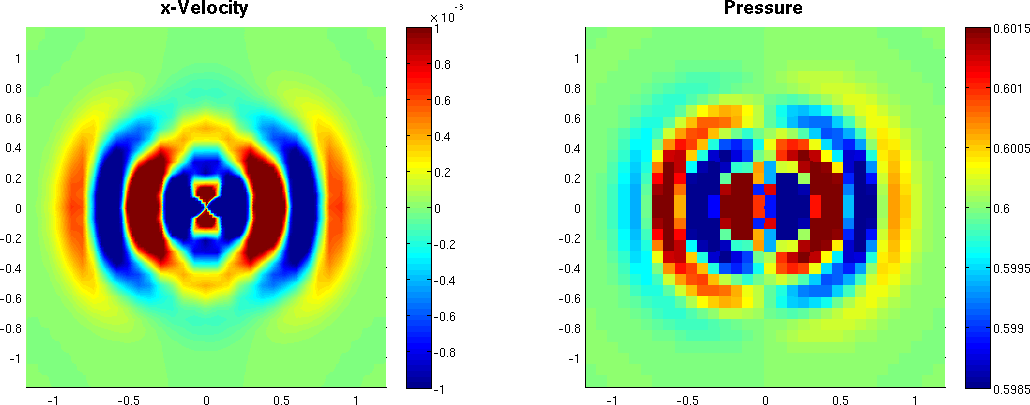
\includegraphics[width=6in,keepaspectratio=true]{./Figures/acousticQ1Q0_hgON.png}
 % elQ1Q0.png: 509x592 pixel, 107dpi, 12.08x14.05 cm, bb=0 0 342 398
 \caption{Traditional \el{Q_1}{Q_0} acoustic wave with hourglass filter}
 \label{fig:acousticwave}
\end{figure}

\section{The \texorpdfstring{\el{Q_1}{Q_0}}{Q1-Q0} Element}
Foremost among our goals is to compare the performance of any new methods with the traditional formulation, the tried and true low order \el{Q_1}{Q_0} element pair. This element has a bi-linear kinematic interpolation and a discontinuous-between-cells constant thermodynamic interpolation. A diagram of the master \el{Q_1}{Q_0} element is shown in \refFig{elQ1Q0}.

\begin{figure}[h!]
 \centering
 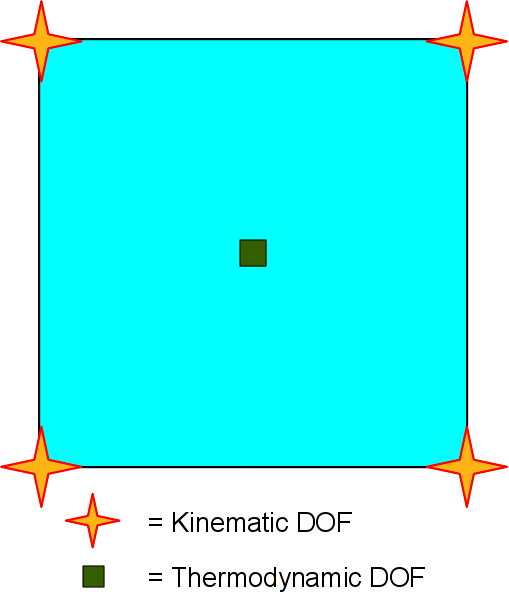
\includegraphics[width=2in,bb=0 0 342 398,keepaspectratio=true]{./Figures/elQ1Q0.png}
 % elQ1Q0.png: 509x592 pixel, 107dpi, 12.08x14.05 cm, bb=0 0 342 398
 \caption{The traditional $Q_1-\hat{Q}_0$ element}
 \label{fig:elQ1Q0}
\end{figure}

\subsection{Assets}
This element has the optimal constrain ratio of $nD$. It is simple and the legacy pair for hydrocodes, hence the theory is well developed and the problems are understood and have mostly been addressed in one form or another. 

\subsection{Liabilities}
This finite element pair has some long-standing issues because it is fundamentally unstable according to the LBB condition. Hourglass/checkerboard modes can render this method useless without an hourglass filter. Even with an hourglass filter, this method requires custom tuning for different problem types because there is no one `safe' value of the hourglass filter. This method is also low order, so it cannot accurately represent curved boundaries.

\subsection{Convergence}
We will be using this method as the `control group' with which we will compare all other methods.

\subsubsection{The $\mathrm{grad}(p)$ Test on a Cartesian Mesh}
On a straight Cartesian mesh the basis function representation of pressure converges linearly with a rate of one. This is what we would expect with piecewise constant pressures. 

The final solution converges at a super-linear rate of 1.52. This can be attributed to the well-documented super-convergence of the \el{Q_1}{Q_0} element  \cite{Douglas1985}. 

\subsubsection{The $\mathrm{grad}(p)$ Test on a Distorted Mesh}
The pressure representation converges with a rate of 1.0 on a a distorted mesh. We don't see any sort of super-convergence with the basis function representation. Thus, we don't see a significant difference between convergence on Cartesian mesh versus a distorted mesh. Henceforth we will report a single value for the convergence of the pressure representation; this will be representative for both meshes. 

With a full mass matrix solve, this method converges under refinement at a rate of 1.4, somewhat better than first order but not quite as fast as second order convergence. We will use this as the baseline to compare all other methods against. 

\subsubsection{The $\mathrm{div}(\mathrm{grad}(V))$ Test on a Cartesian Mesh}
The velocity representation of the continuous vector field converges with a rate of 2.0. This value is representative of both Cartesian and distorted meshes and we will only report one value from now on. 

The calculated accelerations converge to the analytical solution at a quadratic rate of 2.0. 

\subsubsection{The $\mathrm{div}(\mathrm{grad}(V))$ Test on a Distorted Mesh}
On a distorted mesh, the solution converges to a slightly slower rate of 1.52.

\subsection{Spurious Modes}
This finite element pair is notorious for hourglass mode instabilities. In fact, the name ``hourglass mode'' was coined because of how they manifest themselves on this element. \refFig{acousticQ1Q0_hgOFF} illustrates the excited velocity and pressure modes for this basis function pair.

\begin{figure}[h!]
 \centering
 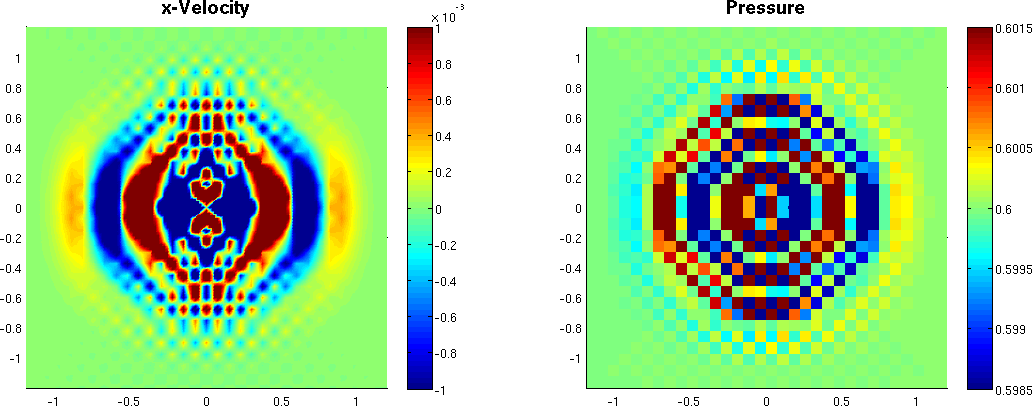
\includegraphics[width=6in,keepaspectratio=true]{./Figures/acousticQ1Q0_hgOFF.png}
 % elQ1Q0.png: 509x592 pixel, 107dpi, 12.08x14.05 cm, bb=0 0 342 398
 \caption{Traditional \el{Q_1}{Q_0} acoustic wave without hourglass filter}
 \label{fig:acousticQ1Q0_hgOFF}
\end{figure}

If we take a closer look at the spurious modes, we will see that they take the familiar hourglass/checkerboard form as illustrated on a patch of four elements in \refFig{hgmodesQ1Q0}.

\begin{figure}[h!]
 \centering
 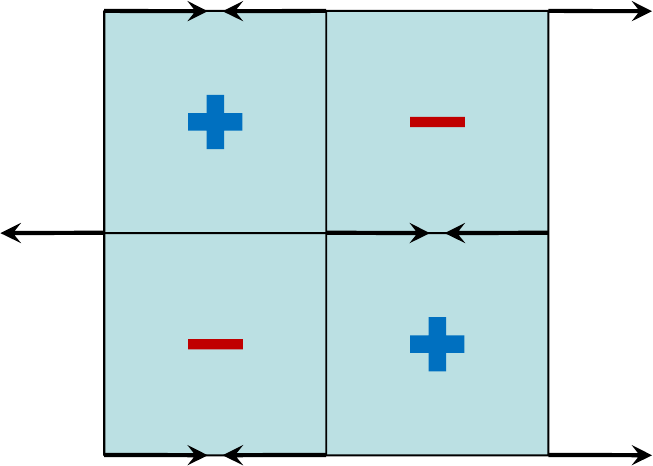
\includegraphics[width=3in,keepaspectratio=true]{./Figures/hgmodesQ1Q0.png}
 % elQ1Q0.png: 509x592 pixel, 107dpi, 12.08x14.05 cm, bb=0 0 342 398
 \caption{Hourglass/checkerboard modes on a patch of \el{Q_1}{Q_0} elements}
 \label{fig:hgmodesQ1Q0}
\end{figure} 

\section{The \texorpdfstring{\el{Q_1}{P_{0r}}}{Q1-P0r} Element}
We include this element in the discussion for the sake of thoroughness, although this element has little potential for a full hydrocode. If we wish to add one more thermodynamic degree of freedom to the \el{Q_1}{Q_0} element, we will get \refFig{elQ1P0r}. There are actually several ways that we could have distributed the two pressure DOFs, none of them great. We could have divided the element in half from top to bottom or left to right, but either of these would have doubled the amount of information in one direction versus the other. We have decided to alternatively split the element down one diagonal then the other. This acts to limit the asymmetry of the mesh.

\begin{figure}[h!]
 \centering
 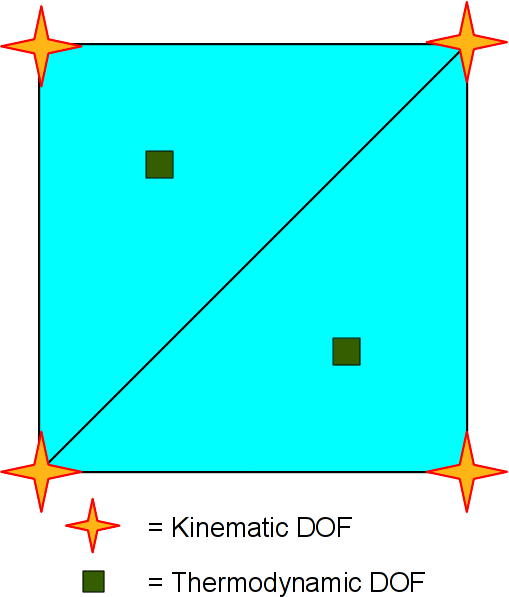
\includegraphics[width=2in,bb=0 0 342 398,keepaspectratio=true]{./Figures/elQ1P0r.png}
 % elQ1Q0.png: 509x592 pixel, 107dpi, 12.08x14.05 cm, bb=0 0 342 398
 \caption{The \el{Q_1}{\hat P_{0r}} element}
 \label{fig:elQ1P0r}
\end{figure}

\subsection{Assets}
This element may initially appear to be a straightforward extension of the traditional \el{Q_1}{Q_0} element. There are no foreseeable  advantages of using this element over any other element. In fact, there are many reasons not to use this element.

\subsection{Liabilities}
In order to limit the inherent asymmetry of this element, it is necessary to alternative placement of the two alternative versions of this element across the mesh. This means changing the software architecture to account for different basis functions depending on whether the element number is even or odd. 

\subsection{Convergence}
The pressure field converges to the exact $\mathrm{grad}(p)$ pressure field at a rate of 1.0, with only slightly less error than \el{Q_1}{Q_0}, as shown in \refFig{gp_cp_convQ1P0r}. The calculated acceleration converges sub-linearly at a rate of 0.54 as shown in \refFig{gp_ca_convQ1P0r}. Apparently, this extra degree of freedom actually slows down the convergence significantly. The $\mathrm{div}(\mathrm{grad}(V))$ convergence will be the same as \el{Q_1}{Q_0}.

\begin{figure}[h!]
 \centering
 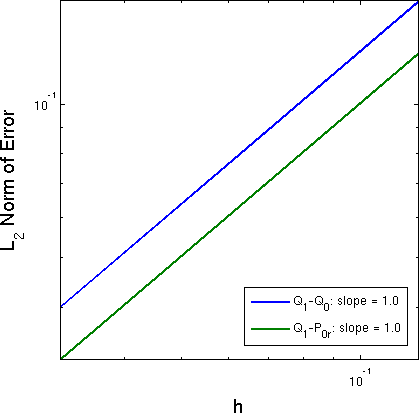
\includegraphics[width=3in,keepaspectratio=true]{./Figures/gp_cp_convQ1P0r.png}
 % elQ1Q0.png: 509x592 pixel, 107dpi, 12.08x14.05 cm, bb=0 0 342 398
 \caption{Convergence of the \el{Q_1}{P_{0r}} pressure field}
 \label{fig:gp_cp_convQ1P0r}
\end{figure}

\begin{figure}[h!]
 \centering
 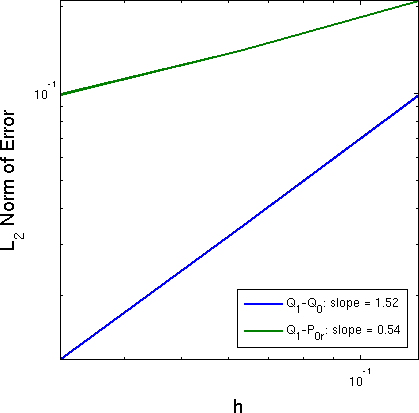
\includegraphics[width=3in,keepaspectratio=true]{./Figures/gp_ca_convQ1P0r.png}
 % elQ1Q0.png: 509x592 pixel, 107dpi, 12.08x14.05 cm, bb=0 0 342 398
 \caption{Convergence of $\Grad p$ acceleration: \el{Q_1}{P_{0r}} versus \el{Q_1}{Q_0} on a Cartesian mesh}
 \label{fig:gp_ca_convQ1P0r}
\end{figure}

\subsection{Spurious Modes}
According to \refFig{acousticQ1P0r_hgOFF}, this element does nothing to eliminate or even reduce spurious velocity and pressure modes.

\begin{figure}[h!]
 \centering
 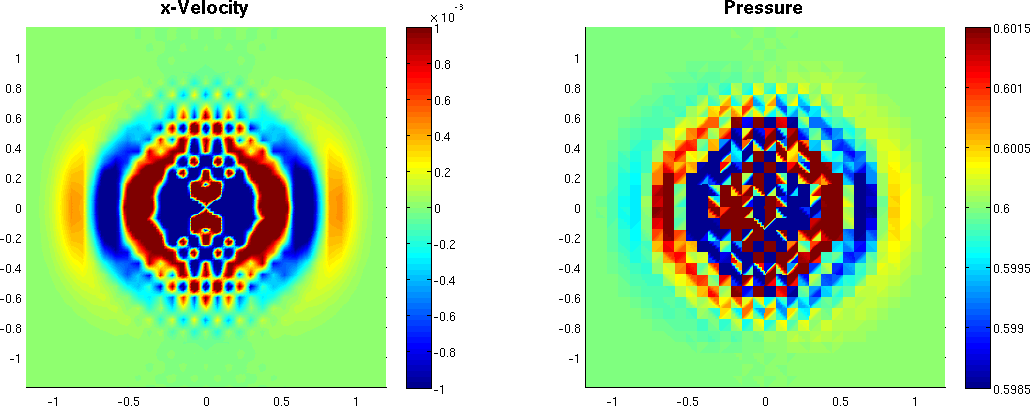
\includegraphics[width=6in,keepaspectratio=true]{./Figures/acousticQ1P0r_hgOFF.png}
 % elQ1Q0.png: 509x592 pixel, 107dpi, 12.08x14.05 cm, bb=0 0 342 398
 \caption{\el{Q_1}{P_{0r}} acoustic wave without hourglass filter}
 \label{fig:acousticQ1P0r_hgOFF}
\end{figure}

\section{The \texorpdfstring{\el{Q_1}{\hat P_1}}{Q1-P1}  Element} \label{sec:Q1P1}
We considered the \el{Q_1}{\hat P_1} and \el{Q_2}{\hat P_1} elements as a means of breaking up the hourglass modes by breaking the symmetry inherent in quad-quad pairs. 

\begin{figure}[h!]
 \centering
 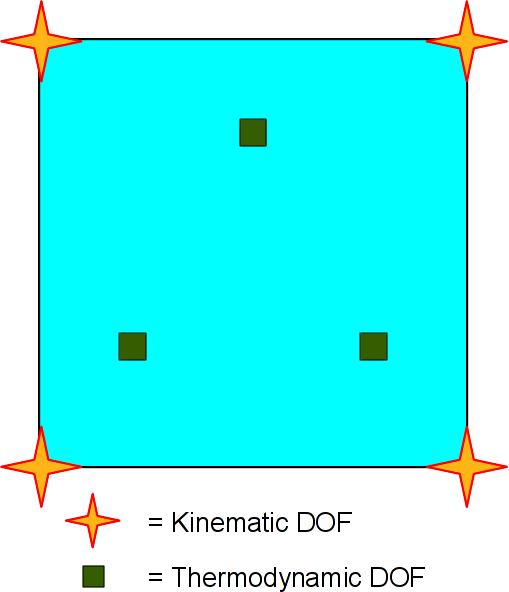
\includegraphics[width=2in,bb=0 0 342 398,keepaspectratio=true]{./Figures/elQ1P1.png}
 % elQ1Q0.png: 509x592 pixel, 107dpi, 12.08x14.05 cm, bb=0 0 342 398
 \caption{The \el{Q_1}{\hat P_1} element}
 \label{fig:elQ1P1}
\end{figure}

After some initial research, it appears that this element behaves identically to the \el{Q_1}{\hat Q_1} element. This actually more of a reflection on \el{Q_1}{\hat Q_1}; it reveals that four pressure degrees of freedom are one too many to be paired with $Q_1$ velocity basis functions. However, because \el{Q_1}{\hat Q_1} has gained so much recognition because of the method of sub-zonal pressures, we will direct our analysis at that element and limit our discussion of \el{Q_1}{\hat P_1} to this: all of the assets, liabilities, and convergence properties of \el{Q_1}{\hat P_1} will be very similar or identical to \el{Q_1}{\hat Q_1}.

\section{The \texorpdfstring{\el{Q_1}{\hat Q_1}}{Q1-Q1} Element}
This element pair, which is illustrated in \refFig{elQ1Q1}, is similar in nature to the method of sub-zonal pressures described by Caramana and Shashkov \cite{CaramanaShashkov98}. The kinematic interpolation is the same as the traditional \el{Q_1}{\hat Q_0} element, but four thermodynamic degrees of freedom are used rather than one. The method of sub-zonal pressures, on the other hand, evolved one pressure degree of freedom and calculated ``sub-zonal pressures'' each time step.

\begin{figure}[h!]
 \centering
 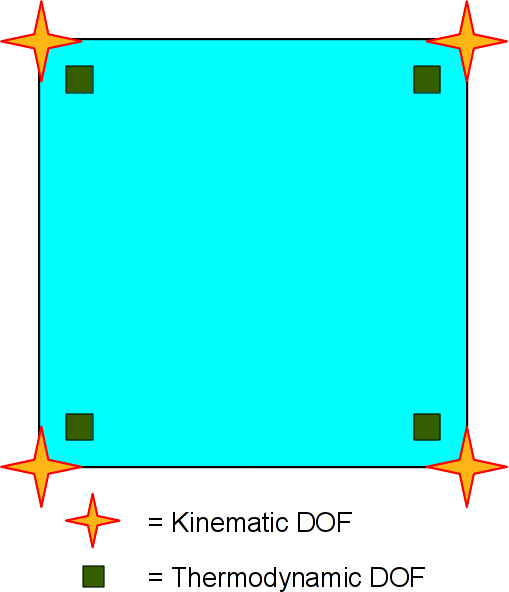
\includegraphics[width=2in,bb=0 0 342 398,keepaspectratio=true]{./Figures/elQ1Q1.png}
 % elQ1Q0.png: 509x592 pixel, 107dpi, 12.08x14.05 cm, bb=0 0 342 398
 \caption{The \el{Q_1}{\hat Q_1} element}
 \label{fig:elQ1Q1}
\end{figure}

\subsection{Assets}
On the surface, this method appears to eliminate checkerboard modes from the pressure field. This seems like it could be an attractively easy fix for checkerboard mode instabilities that does not require special tuning between problems. \refFig{centerPresQ1Q1} shows the resulting average pressures in each cell for the acoustic wave problem.

\begin{figure}[h!]
 \centering
 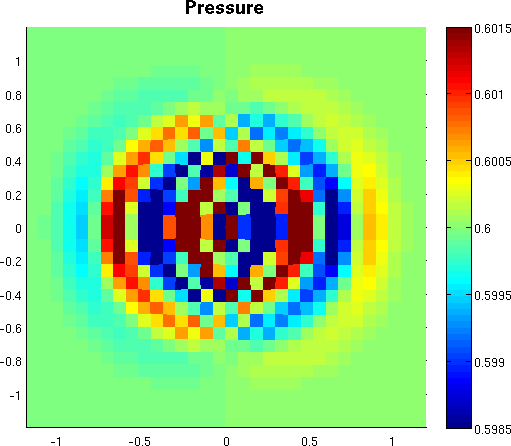
\includegraphics[width=5in,keepaspectratio=true]{./Figures/centerPresQ1Q1.png}
 % elQ1Q0.png: 509x592 pixel, 107dpi, 12.08x14.05 cm, bb=0 0 342 398
 \caption{Average pressure in each cell for \el{Q_1}{\hat Q_1} element for acoustic wave problem}
 \label{fig:centerPresQ1Q1}
\end{figure}

\subsection{Liabilities}
The constraint ratio for this element is $nD/4$, but let's not let that discourage us. We haven't proven whether this is a viable measure of performance yet. We have also shown previously in \refSec{Q1P1} that this element has one too many thermodynamic degrees of freedom. The major downfall of this element comes when we take a closer look at the resulting velocity field. Apparently, \refFig{centerPresQ1Q1} just hid the spurious pressure modes by averaging the pressure degrees of freedom because \refFig{spuriousVQ1Q1} shows that spurious velocity modes in the x- and y- directions. This plot should look more like \refFig{spuriousVQ1Q0}. These spurious modes appear to be more chaotic than \el{Q_1}{Q_0} and may be harder to control.

\begin{figure}[h!]
 \centering
 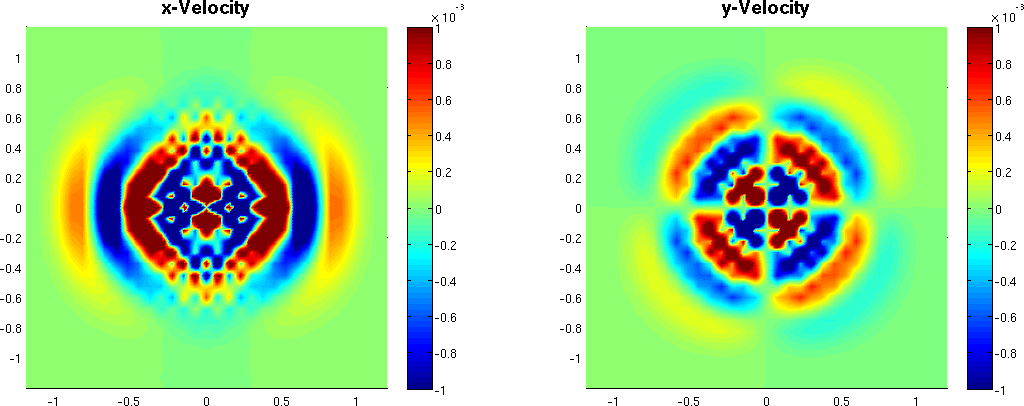
\includegraphics[width=6in,keepaspectratio=true]{./Figures/acousticSpuriousV_Q1Q1.png}
 \caption{Spurious modes in the x- and y-velocity modes with \el{Q_1}{\hat Q_1}}
 \label{fig:spuriousVQ1Q1}
\end{figure}

\begin{figure}[h!]
 \centering
 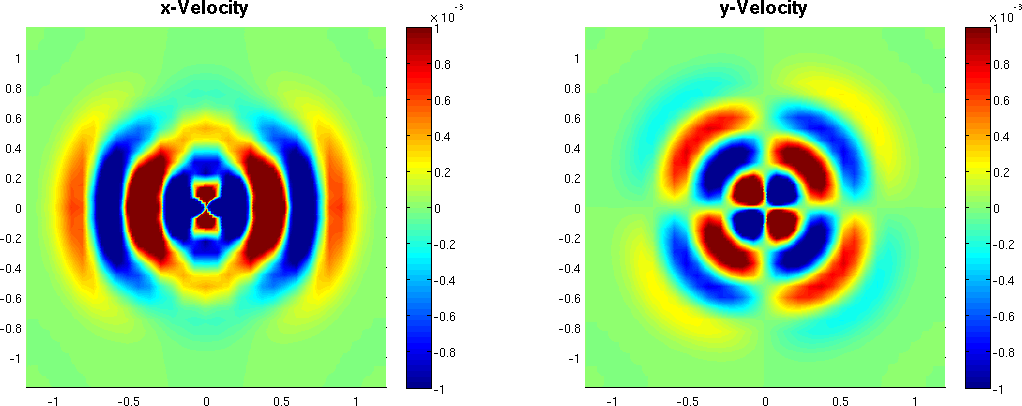
\includegraphics[width=6in,keepaspectratio=true]{./Figures/acousticSpuriousV_Q1Q0.png}
 \caption{Hourglass-free velocity fields with hourglass-filtered \el{Q_1}{Q_0}}
 \label{fig:spuriousVQ1Q0}
\end{figure}

\subsection{Convergence}

\subsubsection{The $\mathrm{grad}(p)$ Test on a Cartesian Mesh}
The pressure representation converges to the continuous pressure field at a quadratic rate of 2.0. This element shares the same pressure representation as the \el{Q_2}{\hat Q_1} element, therefore the pressure field convergence is the same. See \refFig{gp_cp_convQ2Q1} for the convergence of the pressure field of these two elements.

On a Cartesian mesh, the static momentum test converges with a rate of 2.0 as shown in \refFig{gp_ca_convQ1Q1}.

\begin{figure}[h!]
 \centering
 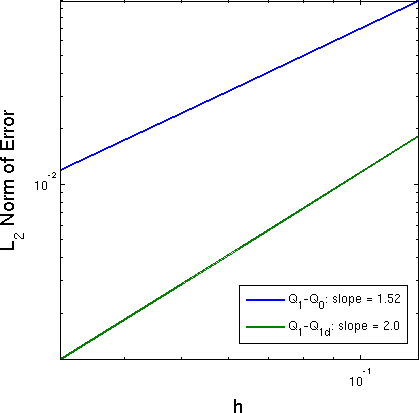
\includegraphics[width=3in,keepaspectratio=true]{./Figures/gp_ca_convQ1Q1.png}
 % elQ1Q0.png: 509x592 pixel, 107dpi, 12.08x14.05 cm, bb=0 0 342 398
 \caption{Convergence of $\Grad p$ acceleration: \el{Q_1}{\hat Q_1} versus \el{Q_1}{Q_0} on a Cartesian mesh}
 \label{fig:gp_ca_convQ1Q1}
\end{figure}

\subsubsection{The $\mathrm{grad}(p)$ Test on a Distorted Mesh}
Despite its deficiencies, this method does converge to the exact solution on a distorted mesh with quadratic convergence as shown in \refFig{gp_da_convQ1Q1}.

\begin{figure}[h!]
 \centering
 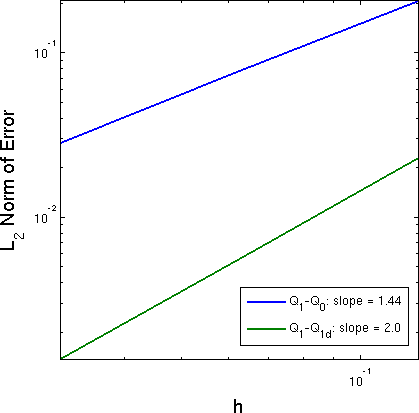
\includegraphics[width=3in,keepaspectratio=true]{./Figures/gp_da_convQ1Q1.png}
 % elQ1Q0.png: 509x592 pixel, 107dpi, 12.08x14.05 cm, bb=0 0 342 398
 \caption{Convergence of $\Grad p$ acceleration: \el{Q_1}{\hat Q_1} versus \el{Q_1}{Q_0} on a distorted mesh}
 \label{fig:gp_da_convQ1Q1}
\end{figure}

\subsubsection{The $\mathrm{div}(\mathrm{grad}(V))$ Test}
It turns out that the stiffness matrix depends entirely on the velocity space. Therefore, the \el{Q_1}{\hat Q_1} element behaves identically to the \el{Q_1}{Q_0} element for $\mathrm{div}(\mathrm{grad}(V))$ test. The pressure space has nothing to do with the results. 

\subsection{Spurious Modes}\label{sec:Q1Q1spuriousmodes}
If we actually plot the bi-linear interpolation of pressure rather than the average value, we will see that the pressure field is not as pretty as we thought. \refFig{acousticQ1Q1_hgOFF} shows the pseudocolor plot for this element on the acoustic wave test.

\begin{figure}[h!]
 \centering
 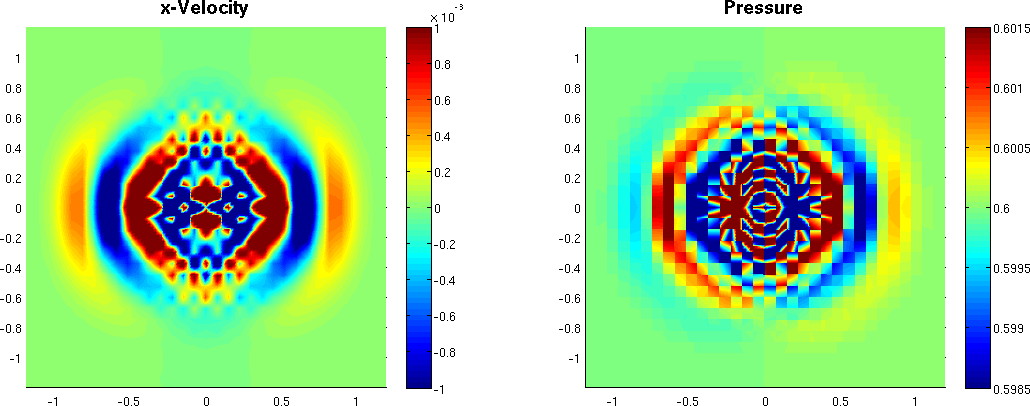
\includegraphics[width=6in,keepaspectratio=true]{./Figures/acousticQ1Q1_hgOFF.png}
 % elQ1Q0.png: 509x592 pixel, 107dpi, 12.08x14.05 cm, bb=0 0 342 398
 \caption{\el{Q_1}{\hat Q_1} acoustic wave without hourglass filter}
 \label{fig:acousticQ1Q1_hgOFF}
\end{figure}

\section{The \texorpdfstring{\el{Q_1}{\hat Q_2}}{Q1-Q2} Element}
In order to be completely thorough, we briefly explored further enriching the pressure space, see \refFig{elQ1Q2}. It turns out that there are not enough velocity DOFs to produce a full bi-quadratic pressure field, but unlike the \el{Q_2}{Q_0} element which has the reverse problem, this is not a fatal flaw. The extra thermodynamic DOFs end up just taking on a bi-linear shape and thus are superfluous. The same problems plague this element as \el{Q_1}{\hat Q_1}.

\begin{figure}[h!]
 \centering
 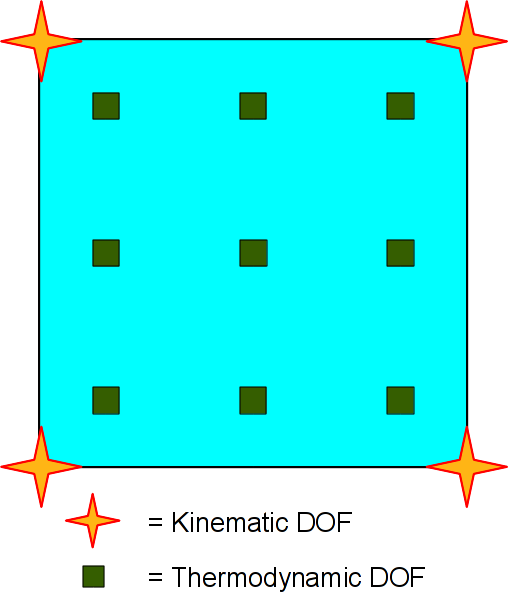
\includegraphics[width=2in,bb=0 0 342 398,keepaspectratio=true]{./Figures/elQ1Q2.png}
 % elQ1Q0.png: 509x592 pixel, 107dpi, 12.08x14.05 cm, bb=0 0 342 398
 \caption{The \el{Q_1}{\hat Q_2} element}
 \label{fig:elQ1Q2}
\end{figure}

\section{The \texorpdfstring{\el{Q_2}{Q_0}}{Q2-Q0} Element}
One of our early attempts to correct hourglass mode instabilities was to follow the lead of some research in Stokes flow and enrich the velocity space. This led to the \el{Q_2}{Q_0} element and caused us to reconsider the applicability of Stokes flow elements to inviscid flow. 

\begin{figure}[h!]
 \centering
 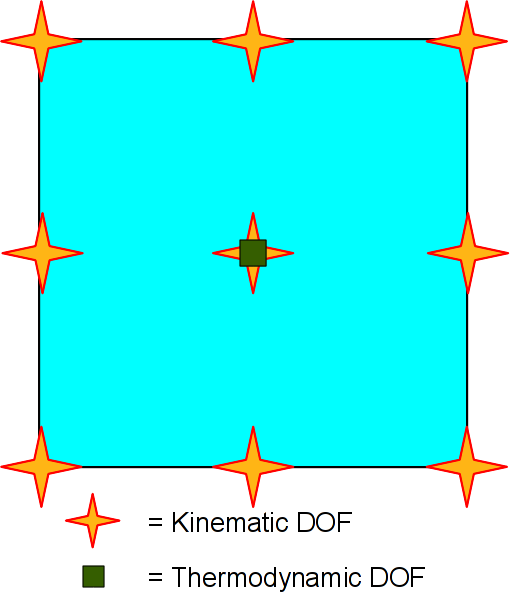
\includegraphics[width=2in,bb=0 0 342 398,keepaspectratio=true]{./Figures/elQ2Q0.png}
 % elQ1Q0.png: 509x592 pixel, 107dpi, 12.08x14.05 cm, bb=0 0 342 398
 \caption{The \el{Q_2}{Q_0} element}
 \label{fig:elQ2Q0}
\end{figure}

\subsection{Assets}
Analysis of the inf-sup condition by Stenberg and Suri \cite{StenbergSuri1996} showed that \el{Q_{k+2}}{Q_k} family of elements is stable for Stokes flow. The \el{Q_2}{Q_0} element falls into this family, but it is not stable for Euler flow.

\subsection{Liabilities}
It turns out that, while this element may work for Stokes flow, there are not enough pressure degrees of freedom to inform the movement of all of the higher order velocity degrees of freedom. The internal degree of freedom, for example, does not ever see any pressure gradient because pressure is constant within each cell. Therefore, the central DOF never moves.

\subsection{Convergence}
This finite element pair does not converge at all, which renders it completely unsuitable for a hydrocode.

\section{The \texorpdfstring{\el{Q_2}{\hat P_1}}{Q2-P1} Element}
One element that showed some unexpected promise was the \el{Q_2}{\hat P_1} element. This element has a bi-quadratic kinematic interpolation and a linear thermodynamic interpolation as depicted in \refFig{elQ2P1}.

\begin{figure}[h!]
 \centering
 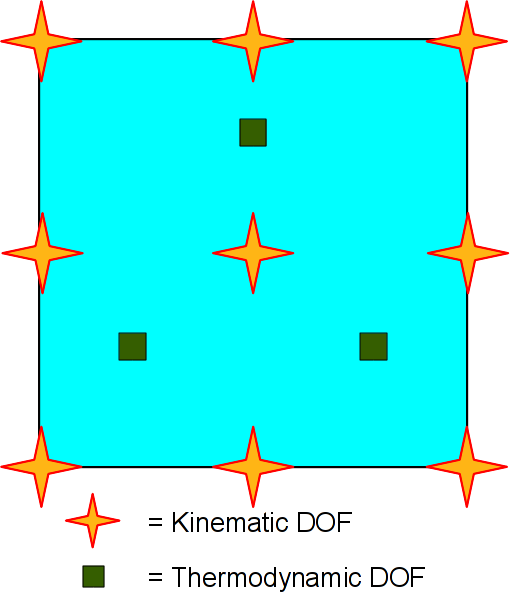
\includegraphics[width=2in,bb=0 0 342 398,keepaspectratio=true]{./Figures/elQ2P1.png}
 % elQ1Q0.png: 509x592 pixel, 107dpi, 12.08x14.05 cm, bb=0 0 342 398
 \caption{The \el{Q_2}{\hat P_1} element}
 \label{fig:elQ2P1}
\end{figure}

\subsection{Assets}
With its bi-quadratic spatial interpolation, this element is capable of producing curved geometries. Similar to the other $Q_2$ elements, this allows us to calculate second derivatives within a single cell while better representing higher-order phenomena with fewer zones and faster convergence. Three pressure DOFs is also the fewest degrees of freedom needed to fully inform the movement of all 9 higher-order velocity degrees of freedom. This means that we can calculate thermodynamic gradients with ease.

\subsection{Liabilities}
Probably the principle oddity of this element lies in the fact that we have ``embedded'' a 3-point basis function on a quadrilateral. There is no real reason why this shouldn't be done, at least for the thermodynamic space, but there is an element of uncertainty about this. If we are using quads, shouldn't we use quad-based basis functions? Where are the most natural locations for these three DOFs? Despite it's higher order nature, this element appears to have slower convergence characteristics on the $\mathrm{grad}(p)$ test than traditional methods. Thus it seems that \el{Q_2}{\hat Q_1} is the preferred higher order method.
% One consequence that could hurt the efficiency of this method is that the thermodynamic DOFs may not line up perfectly with the quadrature points used as 

\subsection{Convergence}
This element has disappointing convergence trends. 

\subsubsection{The $\mathrm{grad}(p)$ Test}
The pressure field representation is the same as for \el{Q_1}{\hat P_1}. The solution converges at a rate of 1.25 which is actually sub-standard compared to \el{Q_1}{Q_0}.

\begin{figure}[h!]
 \centering
 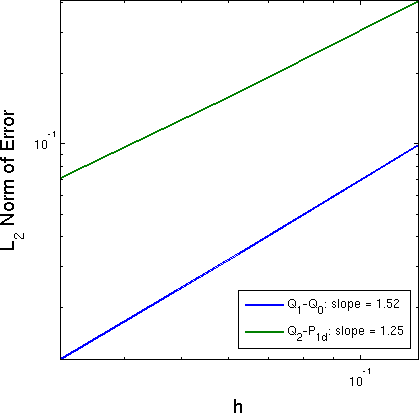
\includegraphics[width=3in,keepaspectratio=true]{./Figures/gp_ca_convQ2P1.png}
 % elQ1Q0.png: 509x592 pixel, 107dpi, 12.08x14.05 cm, bb=0 0 342 398
 \caption{Convergence of $\Grad p$ acceleration: \el{Q_2}{\hat P_1} versus \el{Q_1}{Q_0} on a Cartesian mesh}
 \label{fig:gp_ca_convQ2P1}
\end{figure}

When we distort the mesh, we get an even lower convergence rate of 1.20.

\begin{figure}[h!]
 \centering
 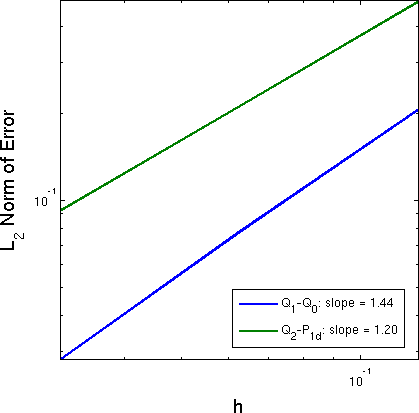
\includegraphics[width=3in,keepaspectratio=true]{./Figures/gp_da_convQ2P1.png}
 % elQ1Q0.png: 509x592 pixel, 107dpi, 12.08x14.05 cm, bb=0 0 342 398
 \caption{Convergence of $\Grad p$ acceleration: \el{Q_2}{\hat P_1} versus \el{Q_1}{Q_0} on a distorted mesh}
 \label{fig:gp_da_convQ2P1}
\end{figure}

\subsubsection{The $\mathrm{div}(\mathrm{grad}(V))$ Test}
Please see \refSec{convdgQ2Q1} for the convergence on the $\mathrm{div}(\mathrm{grad}(V))$ test.

\subsection{Spurious Modes}
The principle benefit of this element over its \el{Q_2}{\hat Q_1} cousin is that the spurious modes appear to be much more low key, see \refFig{acousticQ2Q1_hgOFF} and especially \refFig{acousticQ2Q1_hgON}.

\begin{figure}[h!]
 \centering
 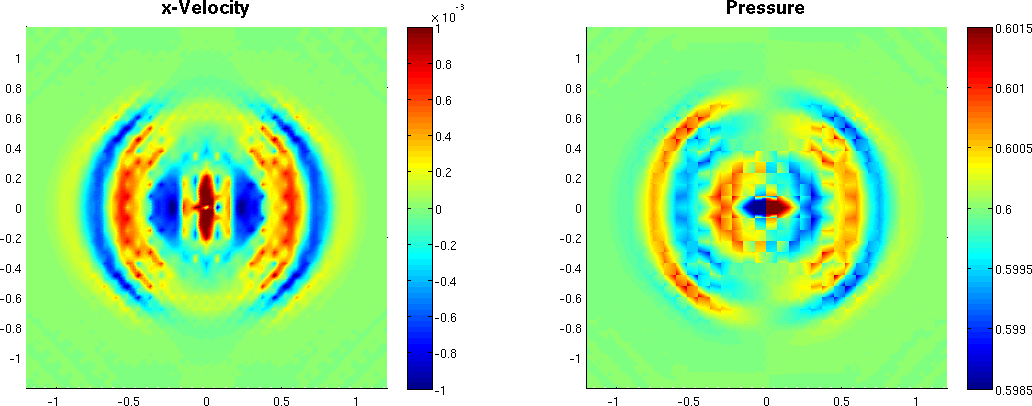
\includegraphics[width=6in,keepaspectratio=true]{./Figures/acousticQ2P1_hgOFF.png}
 % elQ1Q0.png: 509x592 pixel, 107dpi, 12.08x14.05 cm, bb=0 0 342 398
 \caption{\el{Q_2}{\hat P_1} acoustic wave without hourglass filter}
 \label{fig:acousticQ2P1_hgOFF}
\end{figure}

\begin{figure}[h!]
 \centering
 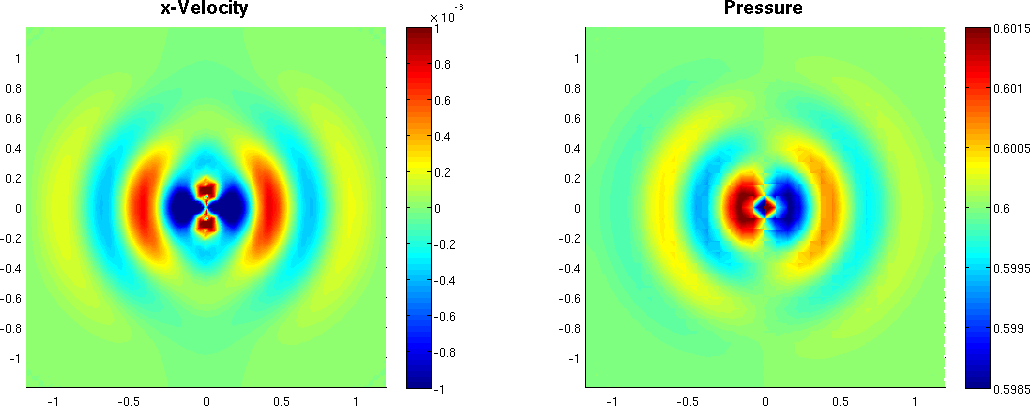
\includegraphics[width=6in,keepaspectratio=true]{./Figures/acousticQ2P1_hgON.png}
 % elQ1Q0.png: 509x592 pixel, 107dpi, 12.08x14.05 cm, bb=0 0 342 398
 \caption{\el{Q_2}{\hat P_1} acoustic wave with hourglass filter}
 \label{fig:acousticQ2P1_hgON}
\end{figure}

\section{The \texorpdfstring{\el{Q_2}{\hat Q_1}}{Q2-Q1} Element}
The logical high-order extension of classical staggered grid hydrodynamics is the \el{Q_2}{\hat Q_1} mixed finite element pair. If we enrich both the kinematic and thermodynamic basis functions by one order, we arrive at a bi-quadratic interpolation for velocity and position and a bi-linear interpolation for pressure, density, and energy, as illustrated in \refFig{elQ2Q1}. This higher order representation of the kinematic variables allows for curvilinear edges and makes it possible to calculate second derivatives within each cell. The bi-linear representation of thermodynamic variables allows us to calculate pressure, energy, and density gradient within each cell. This property could make some sub-zonal physics / multi-material capabilities more straightforward to implement in a full-scale multi-physics hydrocode.

\begin{figure}[h!]
 \centering
 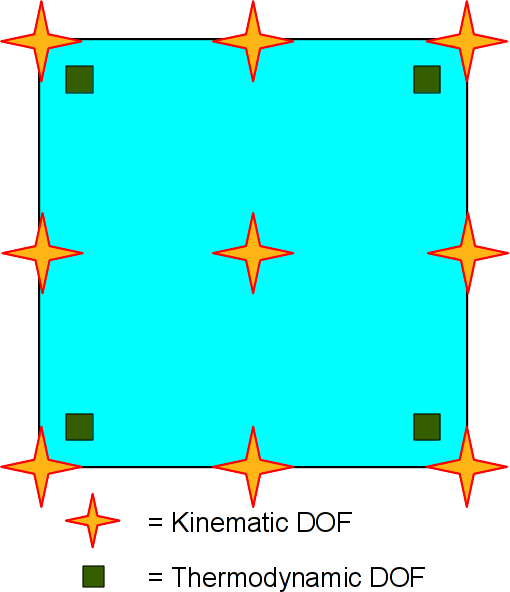
\includegraphics[width=2in,bb=0 0 342 398,keepaspectratio=true]{./Figures/elQ2Q1.png}
 % elQ1Q0.png: 509x592 pixel, 107dpi, 12.08x14.05 cm, bb=0 0 342 398
 \caption{The \el{Q_2}{\hat Q_1} element}
 \label{fig:elQ2Q1}
\end{figure}

\subsection{Assets}
This basis function pair has the optimal constraint ratio of $nD$. This is not a radical departure from traditional SGH; we are only raising the order of each interpolation by one. Therefore this is analogous to a higher order version of traditional SGH, and some of the accumulated knowledge of SGH may carry over to this method. Higher order representations of the variables allow for more accurate calculations and faster convergence while allowing us to model more complicated physics with fewer elements. We will further explore the benefits of this element in \refChap{NumericalResults}

\subsection{Liabilities}
Because this element is analogous to traditional SGH, it shares some of the same pitfalls. For example, hourglass modes take on a very similar, higher order form with \el{Q_2}{\hat Q_1}. Another possible downside to this element is that there are more possible situations where a zero or negative Jacobian could kill a simulation. For example, if the internal DOF moves more than 25\% of the cell length in any direction, the Jacobian will go negative in part of the cell. In practice, for the test problems considered, this has not been a problem, but more study is required. Also, because this is a new method, new analysis must be conducted as to stable time steps, flux between cells during the mesh relaxation stage, etc. We expect a fuller understanding of the pros and cons of this element to come out with time and further study. 

\subsection{Convergence}
This element has an attractive set of convergence properties.

\subsubsection{The $\mathrm{grad}(p)$ Test on a Cartesian Mesh}
The basis function representation of the continuous pressure field converges quadratically with a rate of 2.0 as shown in \refFig{gp_cp_convQ2Q1}.

\begin{figure}[h!]
 \centering
 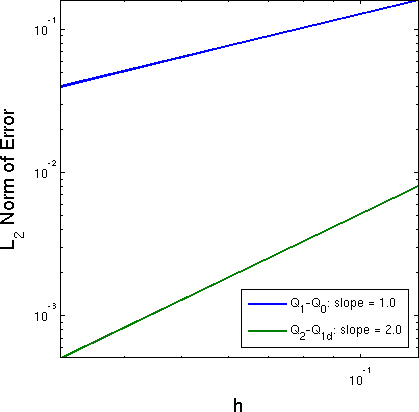
\includegraphics[width=3in,keepaspectratio=true]{./Figures/gp_cp_convQ2Q1.png}
 % elQ1Q0.png: 509x592 pixel, 107dpi, 12.08x14.05 cm, bb=0 0 342 398
 \caption{Convergence of the \el{Q_2}{\hat Q_1} pressure field}
 \label{fig:gp_cp_convQ2Q1}
\end{figure}

On a Cartesian mesh, this element converges quadratically to the analytical solution of the $\mathrm{grad}(p)$ test as shown in \refFig{gp_ca_convQ2Q1}. This is only slightly better than the \el{Q_1}{Q_0} rate of 1.52, but \refFig{gp_ca_convQ2Q1} demonstrates that the actual absolute value of error is much lower.

\begin{figure}[h!]
 \centering
 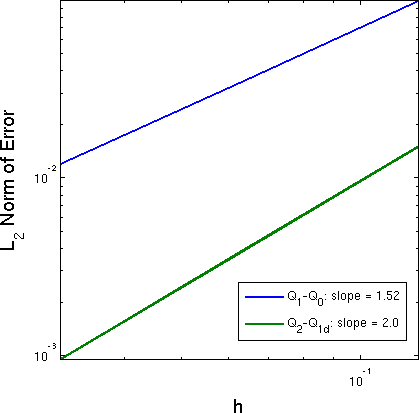
\includegraphics[width=3in,keepaspectratio=true]{./Figures/gp_ca_convQ2Q1.png}
 % elQ1Q0.png: 509x592 pixel, 107dpi, 12.08x14.05 cm, bb=0 0 342 398
 \caption{Convergence of $\Grad p$ acceleration: \el{Q_2}{\hat Q_1} versus \el{Q_1}{Q_0} on a Cartesian mesh}
 \label{fig:gp_ca_convQ2Q1}
\end{figure}

\subsubsection{The $\mathrm{grad}(p)$ Test on a Distorted Mesh}
The convergence on a distorted mesh is the real test of an element because we don't expect to see any perfectly Cartesian meshes in any simulations of real engineering interest. On the distorted mesh, the \el{Q_1}{Q_0} element drops to a rate of 1.44 while the \el{Q_2}{\hat Q_1} element drops to a slightly sub-quadratic convergence of 1.88 as shown in \refFig{gp_da_convQ2Q1}.

Interestingly, even though the \el{Q_2}{\hat Q_1} element has the same pressure space as \el{Q_1}{\hat Q_1}, it doesn't quite maintain the same rate of convergence on a distorted mesh. This difference is minor, but a little unexpected. \refFig{gp_da_convQ1Q1_Q2Q1} compares the convergence of these two elements.

\begin{figure}[h!]
 \centering
 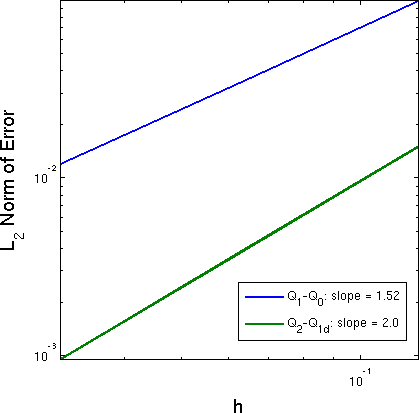
\includegraphics[width=3in,keepaspectratio=true]{./Figures/gp_ca_convQ2Q1.png}
 % elQ1Q0.png: 509x592 pixel, 107dpi, 12.08x14.05 cm, bb=0 0 342 398
 \caption{Convergence of $\Grad p$ acceleration: \el{Q_2}{\hat Q_1} versus \el{Q_1}{Q_0} on a distorted mesh}
 \label{fig:gp_da_convQ2Q1}
\end{figure}

\begin{figure}[h!]
 \centering
 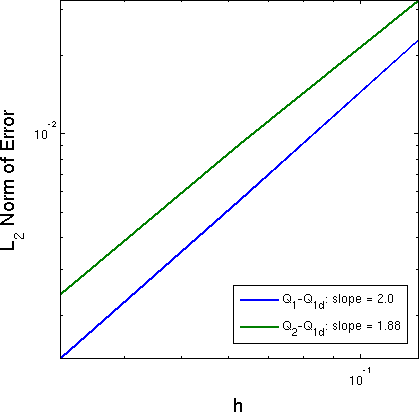
\includegraphics[width=3in,keepaspectratio=true]{./Figures/gp_da_convQ1Q1_Q2Q1.png}
 % elQ1Q0.png: 509x592 pixel, 107dpi, 12.08x14.05 cm, bb=0 0 342 398
 \caption{Convergence of $\Grad p$ acceleration: \el{Q_2}{\hat Q_1} versus \el{Q_1}{Q_1} on a distorted mesh}
 \label{fig:gp_da_convQ1Q1_Q2Q1}
\end{figure}

\subsubsection{The $\mathrm{div}(\mathrm{grad}(V))$ Test on a Cartesian Mesh}\label{sec:convdgQ2Q1}
The velocity projection converges cubically at a rate of 3.0 as shown in \refFig{dg_cV_convQ2Q1}.

\begin{figure}[h!]
 \centering
 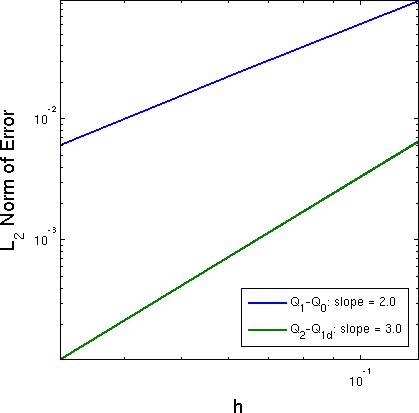
\includegraphics[width=3in,keepaspectratio=true]{./Figures/dg_cV_convQ2Q1.png}
 % elQ1Q0.png: 509x592 pixel, 107dpi, 12.08x14.05 cm, bb=0 0 342 398
 \caption{Convergence of the \el{Q_2}{\hat Q_1} velocity projection vs \el{Q_1}{Q_0}}
 \label{fig:dg_cV_convQ2Q1}
\end{figure}

The \el{Q_2}{\hat Q_1} element converges to the exact solution of the $\mathrm{div}(\mathrm{grad}(V))$ test at a rate of 2.0 on a Cartesian mesh as shown in \refFig{dg_ca_convQ2Q1}. This appears to be somewhat of an anomaly because we expect that the higher order velocity field will result in higher-order convergence.

\begin{figure}[h!]
 \centering
 \includegraphics[width=3in,keepaspectratio=true]{./Figures/dg_ca_convQ2Q1.png}
 % elQ1Q0.png: 509x592 pixel, 107dpi, 12.08x14.05 cm, bb=0 0 342 398
 \caption{Convergence of $\Div\Grad V$ acceleration: \el{Q_2}{\hat Q_1} versus \el{Q_1}{Q_0} on a Cartesian mesh}
 \label{fig:dg_ca_convQ2Q1}
\end{figure}

\subsubsection{The $\mathrm{div}(\mathrm{grad}(V))$ Test on a Distorted Mesh}
On a distorted mesh, the convergence of both \el{Q_1}{Q_0} and \el{Q_2}{\hat Q_1} drop to sub-quadratic convergence of 1.52 and 1.63, respectively as shown in \refFig{dg_da_convQ2Q1}.

\begin{figure}[h!]
 \centering
 \includegraphics[width=3in,keepaspectratio=true]{./Figures/dg_da_convQ2Q1.png}
 % elQ1Q0.png: 509x592 pixel, 107dpi, 12.08x14.05 cm, bb=0 0 342 398
 \caption{Convergence of $\Div\Grad V$ acceleration: \el{Q_2}{\hat Q_1} versus \el{Q_1}{Q_0} on a distorted mesh}
 \label{fig:dg_da_convQ2Q1}
\end{figure}

\subsection{Spurious Modes}
To our disappointment, this element did not eliminate hourglass/checkerboard modes. In fact, the spurious modes present in this element bear a striking resemblance to the traditional hourglass modes found in the \el{Q_1}{Q_0} element. \refFig{acousticQ2Q1_hgOFF} shows the hourglass modes on the acoustic wave test.

\begin{figure}[h!]
 \centering
 \includegraphics[width=6in,keepaspectratio=true]{./Figures/acousticQ2Q1_hgOFF.png}
 % elQ1Q0.png: 509x592 pixel, 107dpi, 12.08x14.05 cm, bb=0 0 342 398
 \caption{\el{Q_2}{\hat Q_1} acoustic wave without hourglass filter}
 \label{fig:acousticQ2Q1_hgOFF}
\end{figure}

If you look closely, you will see that these spurious modes look exactly like a higher frequency version of hourglass modes. The structure of these hourglass modes is illustrated in \refFig{hgmodesQ2Q1}. Compared to some of the other more random spurious modes that we have considered, these more structured modes work to our advantage. They should be easier to analyze and filter, especially considering their similarity to the well-studied \el{Q_1}{Q_0} hourglass modes. You may also notice in comparing \refFig{acousticQ1Q0_hgOFF} and \refFig{acousticQ2Q1_hgOFF}, that the higher frequency modes of \el{Q_2}{\hat Q_1} appear to be of lower magnitude and thus disturb the solution to a smaller degree. Despite the noise from the hourglass modes, we can see a very well defined solution. This will come in handy again as we consider the Sedov explosion test in \refChap{NumericalResults}. If we apply a filter to smooth the hourglass modes,the solution to the acoustic wave problem comes through much clearer in \refFig{acousticQ2Q1_hgON}.

\begin{figure}[h!]
 \centering
 \includegraphics[width=3in,keepaspectratio=true]{./Figures/hgmodesQ2Q1.png}
 % elQ1Q0.png: 509x592 pixel, 107dpi, 12.08x14.05 cm, bb=0 0 342 398
 \caption{Hourglass/checkerboard modes on a patch of \el{Q_2}{\hat Q_1} elements}
 \label{fig:hgmodesQ2Q1}
\end{figure} 

\begin{figure}[h!]
 \centering
 \includegraphics[width=6in,keepaspectratio=true]{./Figures/acousticQ2Q1_hgON.png}
 % elQ1Q0.png: 509x592 pixel, 107dpi, 12.08x14.05 cm, bb=0 0 342 398
 \caption{\el{Q_2}{\hat Q_1} acoustic wave with hourglass filter}
 \label{fig:acousticQ2Q1_hgON}
\end{figure}

This filtered solution looks much better even than the filtered \el{Q_1}{Q_0} solution in \refFig{acousticQ1Q0_hgOFF}.

\section{The \texorpdfstring{\el{Q_2}{\hat Q_2}}{Q2-Q2} Element}
We also tried further refining the thermodynamic space to see what it could buy us. The \el{Q_1}{\hat Q_2} element is a higher order analog of the \el{Q_1}{\hat Q_1} element with both spatial and state variables using a bi-quadratic interpolation. Similar to the \el{Q_1}{\hat Q_2} element, any higher thermodynamic representation like \el{Q_2}{\hat Q_3} appears to be redundant.

\subsection{Assets}
This element shares a lot of the same benefits and handicaps of the \el{Q_1}{\hat Q_1} element. At first glance, if you average the pressure DOFs in each zone, it appears to eliminate checkerboard modes as shown in \refFig{centerPresQ2Q2}, similar to \el{Q_1}{\hat Q_1}. But if we look at the whole picture in \refFig{acousticQ2Q2_hgOFF}, the spurious modes are actually very ugly for this element. We will see in \refSec{nohQ2Q2} that this element appears to arrest density undershoots in the Noh implosion problem. This element also shares the same spatial interpolation with \el{Q_2}{\hat Q_1} which lets this element take on curvilinear geometries. As with \el{Q_2}{\hat Q_1}, we can take second derivatives in space and compute gradients of the thermodynamic fields in a very straightforward way.

\begin{figure}[h!]
 \centering
 \includegraphics[width=5in,keepaspectratio=true]{./Figures/centerPresQ2Q2.png}
 % elQ1Q0.png: 509x592 pixel, 107dpi, 12.08x14.05 cm, bb=0 0 342 398
 \caption{Average pressure in each cell for \el{Q_2}{\hat Q_2} element for acoustic wave problem}
 \label{fig:centerPresQ2Q2}
\end{figure}

\subsection{Liabilities}
This element shares many of the failures of \el{Q_1}{\hat Q_1}, including some serious velocity and pressure modes in the acoustic wave problem as shown in \refFig{acousticQ2Q1_hgOFF}. Similar to \el{Q_2}{\hat Q_1} the Jacobian may be more sensitive to going negative for very deformed meshes.

\subsection{Convergence}
The high order interpolations for spatial and kinematic variables give this element fast convergence rates.

\subsubsection{The $\mathrm{grad}(p)$ Test on a Cartesian Mesh}
The bi-quadratic pressure interpolation converges to the exact pressure field cubically, as demonstrated in \refFig{gp_cp_convQ2Q2}. On a Cartesian mesh, \el{Q_2}{\hat Q_2} converges to the analytical acceleration at a rate of 3.0, as shown in \refFig{gp_ca_convQ2Q2}.

\begin{figure}[h!]
 \centering
 \includegraphics[width=3in,keepaspectratio=true]{./Figures/gp_cp_convQ2Q2.png}
 % elQ1Q0.png: 509x592 pixel, 107dpi, 12.08x14.05 cm, bb=0 0 342 398
 \caption{Convergence of the \el{Q_2}{\hat Q_2} pressure field}
 \label{fig:gp_cp_convQ2Q2}
\end{figure}

\begin{figure}[h!]
 \centering
 \includegraphics[width=3in,keepaspectratio=true]{./Figures/gp_ca_convQ2Q2.png}
 % elQ1Q0.png: 509x592 pixel, 107dpi, 12.08x14.05 cm, bb=0 0 342 398
 \caption{Convergence of $\Grad p$ acceleration: \el{Q_2}{\hat Q_2} versus \el{Q_1}{Q_1} on a Cartesian mesh}
 \label{fig:gp_ca_convQ2Q2}
\end{figure}

\subsubsection{The $\mathrm{grad}(p)$ Test on a Distorted Mesh}
As we can see from \refFig{gp_da_convQ2Q2}, when we distort the mesh, the convergence rate drops down to 2.9.

\begin{figure}[h!]
 \centering
 \includegraphics[width=3in,keepaspectratio=true]{./Figures/gp_da_convQ2Q2.png}
 % elQ1Q0.png: 509x592 pixel, 107dpi, 12.08x14.05 cm, bb=0 0 342 398
 \caption{Convergence of $\Grad p$ acceleration: \el{Q_2}{\hat Q_2} versus \el{Q_1}{Q_1} on a distorted mesh}
 \label{fig:gp_da_convQ2Q2}
\end{figure}

\subsubsection{The $\mathrm{div}(\mathrm{grad}(V))$ Test}
This element has the same velocity space as \el{Q_2}{\hat Q_1}, therefore the convergence rates will be identical for the $\mathrm{div}(\mathrm{grad}(V))$ test.

\subsection{Spurious Modes}
This element has some very ugly spurious modes as we see in \refFig{acousticQ2Q2_hgOFF}. During the process of the solution, it appears that the very noisy interior travels outward from the center at half of the wave speed. Thus as the solution progresses, more and more of it will be overcome by the spurious modes.

\begin{figure}[h!]
 \centering
 \includegraphics[width=6in,keepaspectratio=true]{./Figures/acousticQ2Q2_hgOFF.png}
 % elQ1Q0.png: 509x592 pixel, 107dpi, 12.08x14.05 cm, bb=0 0 342 398
 \caption{\el{Q_2}{\hat Q_2} acoustic wave without hourglass filter}
 \label{fig:acousticQ2Q2_hgOFF}
\end{figure}

\section{Conclusions}
We have considered a large array of different mixed finite element methods in the course of this research, but it would be prohibitive to attempt to do an in-depth study of every one of these elements for every canonical test problem that we will consider. Thus, we need to pair down the search space to a few mixed finite element pairs that showed the most promise. The \el{Q_1}{\hat Q_1} element has been considered in detail in  \cite{CaramanaShashkov98}, so we will carry the results around for comparison. We would like to focus our study on curvilinear elements because they present a new frontier in the field of Lagrangian hydrodynamics. Therefore we will focus primarily on the \el{Q_2}{\hat Q_1} element, which showed the most promise for a full hydrocode. The \el{Q_2}{\hat P_1} element behaves very similarly, so we can assume that most of the discussion concerning \el{Q_2}{\hat Q_1} will apply to this element as well. We will also consider the \el{Q_2}{\hat Q_2} because it represents the higher order analogue of the method of sub-zonal pressures, namely \el{Q_1}{\hat Q_1}. Of course, we need a control to compare against. With that in mind, we will continue to compare against results from traditional \el{Q_1}{Q_0} SGH with and without hourglass filters. % Some Elements Considered

  % Chapter 5

\chapter{Numerical Results} \label{chap:NumericalResults}

In this chapter, we will apply a few selected mixed finite element pairs to several canonical test problems in order to learn how they might perform on real problems of engineering interest. 

\section{The Sod Shock Tube}
The Sod shock tube problem \cite{Sod1978} is a good starting point to check the ability of high order finite element pairs to model shock problems. The Sod shock tube is especially practical because it is one-dimensional, contains both shock waves and expansion fans, and can be solved exactly by means of a Riemann solver \cite{Toro2006}. The problem definition is of two initially static fluids of disparate pressures and densities in a shock tube. The diaphragm is burst, and the higher pressure gas on the left is allowed to expand into the lower pressure gas on the right. This forms two shock waves: one at the interface and the other within the lower density fluid, and one expansion fan in the high density fluid. Solid walls exist at $x=0$ and $x=1$ and the upper and lower boundaries are symmetry plains. The problem is allowed to run until $t=0.6$. The initial problem setup is illustrated in \refFig{SodShockTube}.

\begin{figure}[h!]
 \centering
 \includegraphics[width=5in,keepaspectratio=true]{./Figures/SodShockTube.png}
 % SodShockTube.png: 751x249 pixel, 107dpi, 17.82x5.91 cm, bb=0 0 505 167
 \caption{Problem setup for Sod shock tube problem}
 \label{fig:SodShockTube}
\end{figure}

For this one-dimensional problem, all higher order methods had nearly identical performance. Thus all of our comparisons will be between a single high-order method (\el{Q_2}{\hat Q_1}) and low order \el{Q_1}{Q_0} and assume that \el{Q_2}{\hat Q_2} would have performed similarly. Just to be absolutely clear, there a several little tweaks to \el{Q_1}{Q_0} that we could make to improve the solution, such as implementing a monotonic slope limiter \cite{BergerAftosmis05} or tuning of the \textsf{qquad} and \textsf{qlin} artificial viscosity coefficients. For our comparisons, we have put both elements on an equal footing by setting identical values of $\mathsf{qquad} = 1$ and $\mathsf{qlin}=1$. You will notice that both methods exactly capture the contact discontinuity. This is because the discontinuous nature of the thermodynamic basis functions makes multi-material physics natural and straightforward.

We can learn the most from a set of three plots. It is educational to consider \el{Q_1}{Q_0} on a refined mesh together with \el{Q_2}{\hat Q_1} on a course mesh. The higher-order \el{Q_2}{\hat Q_1} has twice as many DOFs in any direction as \el{Q_1}{Q_0}, so if we use 60 zones for \el{Q_2}{\hat Q_1} and 120 zones for \el{Q_1}{Q_0}, we will have the same total number of DOFs in the $x$-direction. Indeed, if we compare the blue and green lineouts in \refFig{SodCompare}, we see similar behavior despite the disparity in the mesh refinement. Thus we can understand that in general, for \el{Q_1}{Q_0} to achieve comparable accuracy to \el{Q_2}{\hat Q_1} we need twice as many zones in one dimension, four times as many in two dimensions, and eight times as many in three dimensions. This will be an important point when we consider the computational efficiency of each method. Furthermore, if we now consider \el{Q_2}{\hat Q_1} on the same refined mesh as \el{Q_1}{Q_0}, we see a significant improvement in accuracy. Please note the discontinuous behavior of the density plots. The $Q_0$ density climbs the shock in a series of flat steps while $\hat Q_1$ scales it with a smaller series of discontinuous line segments. 

These plots tell us some even more fundamental information about high order mixed finite elements than just accuracy. This first test problem demonstrates the practicality of using high order elements for shock problems. Our greatest fear was that Gibbs phenomenon \cite{Gibbs1898} would cause high frequency ringing around shock discontinuities for high order elements. We will see later that Gibbs phenomenon still occurs for high order elements, but this problem indicates that it may not be as significant an obstacle to overcome as we initially guessed.

\newpage
\begin{figure}[h!]
\begin{textblock*}{7.5in}(.5in,2in)
\centering
   \includegraphics[trim = 0in 3.5in 0in 0in,clip,width=7.5in,keepaspectratio=true]{./Figures/SodCompare.pdf}
\end{textblock*}
\begin{textblock*}{5.5in}(1.5in,8.5in)
\caption{Comparison of \el{Q_1}{Q_0} and \el{Q_2}{\hat Q_1} elements on Sod shock tube and zoomed in on the shock (\textit{right}). Five plot points are considered per zone.}
 \label{fig:SodCompare}
\end{textblock*}
\end{figure}
\mbox{}\clearpage
\newpage

\section{The Noh Implosion}
The Noh implosion problem was first proposed by W. F. Noh \cite{Noh87}. This problem teaches us a lot about symmetry preservation of the method as well as accurate prediction of the shock speed and performance for a very strong shock (shock that decelerates gas to zero velocity). Historically, this problem has posed a significant challenge to bulk artificial viscosity formulations, as demonstrated by \refFig{Noh_MonoQ}, but we have built in the tensor artificial viscosity formulation of Campbell and Shashkov \cite{CampbellShashkov01} and formulated in a finite element sense by Kolev and Rieben \cite{KolevRieben09}. Thus, we should have little problem with symmetry breaking. Hourglass mode interference is minor or negligible for this problem, which allows us to experiment with a 2D shock problem without worrying too much about what effect the hourglass filter is having. In fact, we will be running all of the following cases without any hourglass filtering. Another useful characteristic of the Noh problem is that it has a simple analytical solution for all time, see below.

\begin{eqnarray*}
\vec V &=& \begin{cases}
\vec 0, &\text{for~}r\leq \frac{t}{3}\,, \\
-\hat r, &\text{for~}r > \frac{t}{3}\,.
\end{cases} \\
\rho &=& \begin{cases}
16, &\text{for~}r\leq \frac{t}{3}\,,\\
1 + \frac{t}{r}, &\text{for~}r > \frac{t}{3}\,.
\end{cases} \label{eq:NohAnalytical}\\
p &=& \begin{cases}
16/3, &\text{for~}r\leq \frac{t}{3}\,, \\
0, &\text{for~}r > \frac{t}{3}\,.
\end{cases} \\
\end{eqnarray*}


\begin{figure}[h!]
 \centering
 \includegraphics[width=5in,keepaspectratio=true]{./Figures/Noh2D_MonoQ.png}
 % SodShockTube.png: 751x249 pixel, 107dpi, 17.82x5.91 cm, bb=0 0 505 167
 \caption{Density pseudo-color at time t = 0.6 for the Noh problem on a 40 by 80 initial grid using the monotonic-scalar artificial viscosity.}
 \label{fig:Noh_MonoQ}
\end{figure}

The Noh problem is simple to set up. A uniform gas at zero pressure, with a density of 1.0 and $\gamma=5/3$ is initialized with a unit radially inward velocity at every point in the domain, as illustrated in \refFig{NohImplosion}. As the gas collides at the origin, the density builds up, and a shock wave expands radially outward at a speed of 1/3. There is one particular feature of this test problem that has plagued Lagrangian codes since its inception. ``Wall heating,'' which is caused by numerical shocks repeatedly reflecting through the zone at the origin causes that first cell to have a drastically lower density than it should \cite{Rider2000}. This is unavoidable for a simple research code such as \texttt{Fermium}, and is not a function of the finite element pair chosen, but purely of the framework (Eulerian or Lagrangian). We will just need to acknowledge its presence and then look past it.

It should be immediately obvious that we don't actually have to model this entire domain. One quadrant should be sufficient to obtain all the information we need. Therefore for this and the Sedov problem, we will only model the first quadrant and define the bottom and left boundaries to be symmetry plains. 

\begin{figure}[h!]
 \centering
 \includegraphics[width=3.5in,keepaspectratio=true]{./Figures/NohImplosion.png}
 % SodShockTube.png: 751x249 pixel, 107dpi, 17.82x5.91 cm, bb=0 0 505 167
 \caption{Problem setup for Noh implosion problem}
 \label{fig:NohImplosion}
\end{figure}

\subsection{Low Order \texorpdfstring{\el{Q_1}{Q_0}}{Q1-Q0}}
We require a huge number of low order elements to get anywhere close to the exact solution of the Noh problem. The original shock heating appears to irreparably damage the solution, dragging the predicted density way below the correct value and offsetting the shock past its correct position, see \refFig{Noh_Q1Q0_20x20_hgOFF}. The \el{Q_1}{Q_0} solution does have this going for it however, it does not undershoot or overshoot the solution at the shock front. This lends favorably to the stability of the method because we never see negative pressures or densities show up in the solution. We also consider a refined 40$\times$40 solution in \refFig{Noh_Q1Q0_40x40_hgOFF} in order to observe the convergence to the analytical solution.

\NohPlot{Q1Q0}{20}{OFF}{\el{Q_1}{Q_0}}{without}
\NohPlot{Q1Q0}{40}{OFF}{\el{Q_1}{Q_0}}{without}

\subsection{Low Order \texorpdfstring{\el{Q_1}{\hat Q_1}}{Q1-Q1}}
Now turning to the \el{Q_1}{\hat Q_1} element, we can see some promising results from the Noh problem, as illustrated by \refFig{Noh_Q1Q1_20x20_hgOFF}. We still don't achieve the desired post-shock density, but the solution looks very reasonable and stable overall. The post-shock density field looks especially uniform compared to \el{Q_2}{\hat Q_1} and \el{Q_2}{\hat Q_2}. Even with the refined 40$\times$40 mesh, the density doesn't quite reach the correct value, but the field is pretty good overall. Sharing the same kinematic basis functions, the velocity field is very similar to \el{Q_1}{Q_0}.

\NohPlot{Q1Q1}{20}{OFF}{\el{Q_1}{\hat Q_1}}{without}
\NohPlot{Q1Q1}{40}{OFF}{\el{Q_1}{\hat Q_1}}{without}

\subsection{High Order \texorpdfstring{\el{Q_2}{\hat Q_1}}{Q2-Q1}}
We see a marked improvement when we switch to higher order, as illustrated by \refFig{Noh_Q2Q1_20x20_hgOFF}. Both the velocity and density plots get a lot closer to the exact solution, but we also start to see some troubling features. The density scatter plot shows some huge overshoots and undershoots oscillating around the shock front, we also get some small overshoots in the velocity plot. This is slightly troubling because we actually see density dip below the x-axis to some negative values. The average density in each cell would still be positive, but even a negative interpolation is cause for concern. Indeed, it is very important that we address this if we ever wish to implement a high-order Lagrangian hydro code. We have observed that this oscillation can be controlled through adjustment of the artificial viscosity coefficients, but this also significantly smears out the shock. The concept of hyperviscosity, as postulated by Cook and Cabot \cite{CookCabot2004,CookCabot2005} shows particular promise at eliminating shock oscillations for higher order methods. This method uses multiplications of the stiffness matrix to filter out non-physical oscillatory behavior with a minimal number of problem dependent constants. Please note the significant improvement in the matching capability of the density plot. While a 40$\times$ by \el{Q_1}{Q_0} mesh fails to accurately predict the post-shock density, a mere 20$\times$20 \el{Q_2}{\hat Q_1} hits it right on the head. Although the oscillations get worse under refinement, the overall solution gets much closer to the analytic prediction under refinement as we can see in \refFig{Noh_Q2Q1_40x40_hgOFF}. The velocity matching is the closest of anything that we have seen so far. 

\NohPlot{Q2Q1}{20}{OFF}{\el{Q_2}{\hat Q_1}}{without}
\NohPlot{Q2Q1}{40}{OFF}{\el{Q_2}{\hat Q_1}}{without}

\subsection{High Order \texorpdfstring{\el{Q_2}{\hat Q_2}}{Q2-Q2}}\label{sec:nohQ2Q2}
The benefit of this element chiefly lies in its ability to avoid density undershoots at the shock front. The bi-quadratic density and pressure fields must give a single element the flexibility to jump from a low to a high density  without overshooting both directions while still maintaining the correct mass within that zone. The density overshoots on the other hand, are more more severe than the \el{Q_2}{\hat Q_1} element. The velocity field is much the same as its \el{Q_2}{\hat Q_1} cousin.

\NohPlot{Q2Q2}{20}{OFF}{\el{Q_2}{\hat Q_2}}{without}
\NohPlot{Q2Q2}{40}{OFF}{\el{Q_2}{\hat Q_2}}{without}

\section{The Saltzman Piston}
The Saltzman piston problem \cite{Saltzman1985,Gryra1992} is commonly used to test the effectiveness of new artificial viscosity schemes. In this problem a one-dimensional piston driven shock propagates through a two-dimensional mesh that has been perturbed according to \refEq{SaltzmanPert}. We applied this transformation to a 50$\times$10 mesh with original width and height of 1.0 and 0.1, as shown in \refFig{SaltzmanMesh}. This tests the ability of a method to model shock waves that are not aligned with the mesh. The tensor artificial viscosity formulation has already been tested on the Saltzman piston by  \cite{CampbellShashkov01},  \cite{KolevRieben09}, and  \cite{Lipnikov2010}, but we aim to demonstrate the effectiveness of high order elements on this problem.

\newEq{SaltzmanPert}{
x(i,j)=(i-1)\frac{x_{max}-x_{min}}{NZ_x}+(NZ_y+1-j)\sin\left(\frac{\pi(i-1)}{NZ_x}\right)\frac{y_{max}-y_{min}}{NZ_y}}

\begin{figure}[h!]
 \centering
 \includegraphics[width=6in,keepaspectratio=true]{./Figures/SaltzmanMesh2.png}
 % SodShockTube.png: 751x249 pixel, 107dpi, 17.82x5.91 cm, bb=0 0 505 167
 \caption{Initial perturbed Saltzman piston mesh}
 \label{fig:SaltzmanMesh}
\end{figure}

The domain is initially filled with an ideal gas ($\gamma=5/3$) of density 1 and zero pressure. A piston enters from the left side at a constant speed of 1.0 which generates a shock that reaches the right wall at $t=0.8$ and reflects off the left wall again at $t=0.9$. We run the simulation to a time of 0.925 which stops the simulation shortly before the shock reaches the right wall a second time. The analytical pre- and post-shock densities are 10 and 20, respectively. Similar to Noh, this problem also suffers from ``wall heating'' and the low right and left densities should be overlooked. 

\subsection{Low Order \texorpdfstring{\el{Q_1}{Q_0}}{Q1-Q0}}
The tensor artificial viscosity allows this solution to progress smoothly without the mesh tangling that we see with bulk artificial viscosity formulations \cite{Barlow07}. The shock front is a little jagged because the shock must tackle a whole piece-wise constant density cell at a time rather than smoothly traversing it with a bi-linear or bi-quadratic thermodynamic interpolation. Thus the shock gets ahead of itself at points and behind in others. When we look at the hourglass filtered solution, we see our first evidence that hourglass filters should not be arbitrarily applied with equal magnitude to every problem. They must be tuned for each simulation, and herein lies their Achilles heel. The simulationist must invest a significant amount of time running and rerunning any new problem to determine the optimal hourglass filter setting. We seek either a filter that does not require tuning or preferably an element pair that will be naturally hourglass free. We have not yet arrived at a suitable solution. \refFig{Saltzman_Q1Q0_50x10_hgON} demonstrates that an hourglass filter can do more to harm a solution than to fix it. Even without an hourglass filter, we see some post-shock waves in the mesh where we should see horizontal lines.

\SaltzmanPlot{Q1Q0}{}{OFF}{\el{Q_1}{Q_0}}{without}
\SaltzmanPlot{Q1Q0}{}{ON}{\el{Q_1}{Q_0}}{with}

\subsection{Low Order \texorpdfstring{\el{Q_1}{\hat Q_1}}{Q1-Q1}}
We get some very positive results when we update to a bi-linear thermodynamic space. The additional pressure and density information allows the shock to move through the domain with less interference to the mesh. In \refFig{SaltzmanD_Q1Q1_50x10_hgOFF} we can see certain zones partly shocked while one corner remains in its pre-shock condition. Similar to \el{Q_1}{Q_0}, we also see some incorrect post-shock waves in the mesh. Overall, however, this is a very solid solution.

\SaltzmanPlot{Q1Q1}{}{OFF}{\el{Q_1}{\hat Q_1}}{without}
% \SaltzmanPlot{Q1Q1}{}{ON}{\el{Q_1}{\hat Q_1}}{with}

\subsection{High Order \texorpdfstring{\el{Q_2}{\hat Q_1}}{Q2-Q1}}
Looking primarily at the mesh, \el{Q_2}{\hat Q_1} produces the best solution so far. The horizontal mesh lines are straighter than and the shock more uniform than any of the lower order results. The shock has a lot more flexibility to travel unimpeded across each cell layer because of high order information within each zone. The shock itself is very sharp with some velocity overshoots and significant density overshoots. The chief failing of this method is in the manifestation of the hourglass modes. Indeed, this simulation will not run to completion without an hourglass filter. We see the opposite scenario with the Sedov problem - \el{Q_1}{Q_0} will not run without and hourglass filter, but \el{Q_2}{\hat Q_1} will. This further illustrates the unpredictable nature of hourglass modes. It is very hard to tell if and when they will throw a wrench in a simulation. 

\SaltzmanPlot{Q2Q1}{}{ON}{\el{Q_2}{\hat Q_1}}{with}

\subsection{High Order \texorpdfstring{\el{Q_2}{\hat Q_2}}{Q2-Q2}}
A higher order thermodynamic field allows us to run the simulation to completion without an hourglass mode, but we still see evidence of near failure at the shock front near the top surface. A near mesh-collapse has produced a ``hot spot'' of very high density and pressure. Aside from this, the mesh looks very good with relatively straight horizontal mesh lines. We get a more stable solution with an hourglass filter except for an anomalous ``cold spot'' in the center of the post-shock velocity field. With an hourglass filter, the overall solution appears to be superior to the low order methods but inferior to the \el{Q_2}{\hat Q_1} results with an hourglass filter. 

\SaltzmanPlot{Q2Q2}{}{OFF}{\el{Q_2}{\hat Q_2}}{without}
\SaltzmanPlot{Q2Q2}{}{ON}{\el{Q_2}{\hat Q_2}}{with}

\section{The Sedov Blast Wave}
The previous problems were informative, but they did not allow us to demonstrate the true power of high order elements - curvilinear zones. The Sedov explosion problem \cite{Sedov59} brings these curvilinear capabilities to the forefront. In two dimensions, the Sedov problem is a point-blast wave in an initially static ideal gas medium of constant density, zero pressure, with a delta function initial source of energy at the origin, as illustrated in \refFig{SedovExplosion}. In plain terms, this a simplification of an explosion: a lot of energy is released in a small area and then it expands into the surrounding domain. The problem runs to $t$=1.0 which allows the shock wave to expand to a radius of 1.0.

\begin{figure}[h!]
 \centering
 \includegraphics[width=3in,keepaspectratio=true]{./Figures/SedovExplosion.png}
 % SodShockTube.png: 751x249 pixel, 107dpi, 17.82x5.91 cm, bb=0 0 505 167
 \caption{Problem setup for Sedov blast wave problem}
 \label{fig:SedovExplosion}
\end{figure}

We mentioned previously that the Sedov blast wave presents one of the most compelling arguments for using curvilinear elements. By its very nature, this problem seeks to curve geometries that may have been initially Cartesian. Indeed, when we apply the exact solution of this problem to an initially Cartesian grid, as we do in \refFig{CartSedov}, it becomes obvious that anything other than curvilinear elements would introduce undesirable inaccuracies into the mesh geometry, even under refinement.

\begin{figure}[h!]
 \centering
 \includegraphics[width=5in,keepaspectratio=true]{./Figures/sedovCart.png}
 % SodShockTube.png: 751x249 pixel, 107dpi, 17.82x5.91 cm, bb=0 0 505 167
 \caption{Exact solution to the Sedov problem applied to an initially Cartesian grid}
 \label{fig:CartSedov}
\end{figure}

\subsection{Low Order \texorpdfstring{\el{Q_1}{Q_0}}{Q1-Q0}}
Historically, this problem has presented significant challenges to \el{Q_1}{Q_0} because hourglass mode instabilities cause the solution to crash if they are not filtered out. We would like to compare each of our methods with and without an hourglass filter, but it is simply impossible to obtain an hourglass filter-less solution with \el{Q_1}{Q_0}. If we do apply an hourglass filter we are able to get a stable solution, as seen in\refFig{Sedov_Q1Q0_10x10_hgON} with a very coarse 10$\times$10 mesh.

The Sedov problem is inherently circular. A point source of energy should produce a circular blast wave expanding out from the origin. Therein we see a significant limitation of low order methods. We are only able to produce straight-edged elements with \el{Q_1}{Q_0} which interfere with the curved nature of the problem. With this coarse mesh we can see how the zone at the origin (which doesn't have enough DOFs to represent a curved edge) induces an kinked shock wave where we should see a nice smooth radius. This problem can be mitigated by adding more elements, but it still exists as a significant source of error when modeling fundamentally curved phenomena.

You will also notice that the shock has been smeared considerably. This is primarily the fault of the piece-wise constant representation for density and pressure. We can thank artificial viscosity for smoothing the shock discontinuity out enough to allow a numerical solution, but we still expect to see sharp gradients of density, pressure, and velocity. The low order method can only take one step in density or pressure per zone, thus we see the shock being spread over several zones to smooth out the sharp change in value. We can alleviate this shock smoothing by tweaking the artificial viscosity coefficients, but the fact remains that low order methods are fundamentally limited in their ability to capture sharp gradients.

This low order representation of density and pressure also limits our ability to accurately predict the maximum density and pressure in the shock wave. The constant density interpolation is only able to represent averages over a zone without any additional fluctuations within that zone. Thus, for rapidly changing phenomena like a blast wave, we are very limited in what we can learn without extensive mesh refinement.

We are able to see nominal improvement if we double the resolution in both the $x$- and $y$- directions, as seen in \refFig{Sedov_Q1Q0_20x20_hgON}. While higher resolution attains closer correspondence to the exact solution, the density spike is still grossly under-predicted, and the zone at the origin is still fails to resemble the exact solution in \refFig{CartSedov}.

\SedovPlot{Q1Q0}{10}{ON}{\el{Q_1}{Q_0}}{with}
\SedovPlot{Q1Q0}{20}{ON}{\el{Q_1}{Q_0}}{with}

\subsection{Low Order \texorpdfstring{\el{Q_1}{\hat Q_1}}{Q1-Q1}}
As discussed previously, the main benefit of the \el{Q_1}{\hat Q_1} element is that it appears to squelch hourglass modes in certain situations. We saw in \refSec{Q1Q1spuriousmodes} that this element introduces new spurious modes, but in the Sedov problem, at least, these modes appear to be negligible. The immediate improvement we see when we compare the 10$\times$10 results to \el{Q_1}{Q_0} is that the higher order density field allows the shock to better maintain a circular shape. This results in a more tightly grouped, and hence more accurate, velocity scatter plot. The density results also adhere more closely to the exact solution, approaching closer to the peak value. Despite the straight-edged zones, this is a very good solution overall, and it only gets better with more elements. The shock is still more blurred than higher order methods can give us and the density still does not quite reach the accurate peak value.

\SedovPlot{Q1Q1}{10}{OFF}{\el{Q_1}{\hat Q_1}}{without}
\SedovPlot{Q1Q1}{20}{OFF}{\el{Q_1}{\hat Q_1}}{without}

\subsection{High Order \texorpdfstring{\el{Q_2}{\hat Q_1}}{Q2-Q1}}
The most prominent feature of the \el{Q_2}{\hat Q_1} solution is the curved original zone. Without an hourglass filter it looks almost as if it were bowing out from the force of the explosion. This bowing is actually non-physical, but the overall curvature of the element lends very favorably to the accuracy of the scheme. We also see post-shock oscillations in the velocity field. Despite these hourglass-based penalties, the shock capturing is much sharper. At many points we can see the entire shock captured within one zone. 

If we apply a simple hourglass filter by leaving 25\% of linear artificial viscosity term on in expansion, the results look very fine indeed. The curved zones are reminiscent of the exact solution of the mesh geometry in \refFig{CartSedov}. This also eliminates the oscillations and gives us a solution very close the exact. The results only get better under refinement. At 20$\times$20 mesh refinement, we see very little variation from the exact answer.

In order to completely level the playing field concerning the limitations of \el{Q_1}{Q_0} for curved geometries, we should consider the same problem using the same number of DOFs with curvilinear elements. One of the most significant limitations of low order elements on the Sedov problem was that for a coarse enough grid (10$\times$10), the zone at the origin induced a kinked shape on the shock wave downstream. If we wish to compare this result with curvilinear elements with the same number of DOFs, we would need to use the almost absurd mesh resolution of 5$\times$5. We can see in \refFig{Sedov_Q2Q1_5x5_hgON} that this coarse \el{Q_2}{\hat Q_2} solution avoids the angular mesh problem and produces a surprisingly symmetric and reasonable result.

\SedovPlot{Q2Q1}{10}{OFF}{\el{Q_2}{\hat Q_1}}{without}
\SedovPlot{Q2Q1}{10}{ON}{\el{Q_2}{\hat Q_1}}{with}
\SedovPlot{Q2Q1}{20}{ON}{\el{Q_2}{\hat Q_1}}{with}

\SedovPlot{Q2Q1}{5}{ON}{\el{Q_2}{\hat Q_1}}{with}

We gain some further insight when we run this simulation on a full mesh, and instead of splitting up the energy source into four cells, we energize a single cell which encompasses the origin. We can see the results of two 21$\times$21 runs in \refFig{SedovFullMeshCompare}. The \el{Q_1}{Q_0} elements lack the flexibility to expand naturally from the force of the explosion, hence the original zone is forced to retain its square shape as it expands. This imposes a square shock front and causes the corner elements to bend unnaturally until one of the corners exceeds a 180 degrees at $t$=0.868. This causes the Jacobian to go negative and the solution to go unstable and the simulation to stop. The bi-quadratic method, on the other hand, possesses the required flexibility to expand naturally with the force of the explosion, and the simulation progresses smoothly to the end at $t$=1.0. This is a rather extreme test, but curvilinear elements displays a distinct advantage of straight-edged methods. 

\begin{figure}[h!]
 \centering
 \includegraphics[width=6in,keepaspectratio=true]{./Figures/SedovFullMeshCompare.png}
 % SodShockTube.png: 751x249 pixel, 107dpi, 17.82x5.91 cm, bb=0 0 505 167
 \caption{Comparison of \el{Q_1}{Q_0} (\textit{left}) and \el{Q_2}{\hat Q_1} (\textit{right}) on a full 21$\times$21 mesh.}
 \label{fig:SedovFullMeshCompare}
\end{figure}

% \clearpage
% \newpage
% \begin{figure}[ht]
% \begin{textblock*}{7in}(.75in,1in)
% \centering
% \subfigure[Velocity magnitude pseudocolor plot (\textit{left}). Velocity magnitude scatter plot compared to exact solution (\textit{right}).]{
% \includegraphics[width=7in,keepaspectratio=true]{./Figures/FullMesh/SedovV_Q2Q1_21x21_hgON}
% \label{fig:SedovV_#1_#2x#2_hg#3}
% }
% \subfigure[Density pseudocolor plot (\textit{left}). Density scatter plot compared to exact solution (\textit{right}).]{
% \includegraphics[width=7in,keepaspectratio=true]{./Figures/FullMesh/SedovD_Q2Q1_21x21_hgON}
% \label{fig:SedovD_#1_#2x#2_hg#3}
% }
% \caption{Sedov explosion problem on 21$\times$21 full mesh using \el{Q_2}{\hat Q_1} elements with hourglass filtering}
% \label{fig:Sedov_#1_#2x#2_hg#3}
% \end{textblock*}
% \end{figure}
% \clearpage
% \newpage

\subsection{High Order \texorpdfstring{\el{Q_2}{\hat Q_2}}{Q2-Q2}}
\el{Q_2}{\hat Q_2} does not perform quite as admirably for this problem. Without an hourglass filter we get some velocity ``hot spots'' at the symmetry boundaries and despite its higher order potential, the original zone is not nearly curved enough. It almost looks like one of the lower order solutions. The situation actually gets worse under refinement. The original cell and many layers beyond actually bow inward, a phenomenon that is completely non-physical. We also start to see some very bad noise in the velocity plot. This just goes to show the unpredictable nature of the \el{Q_2}{\hat Q_2} element. In some cases it appears to squelch hourglass modes, but in others spurious modes run rampant. The solution improves dramatically with an hourglass filter.

\SedovPlot{Q2Q2}{10}{OFF}{\el{Q_2}{\hat Q_2}}{without}
% \SedovPlot{Q2Q2}{10}{ON}{\el{Q_2}{\hat Q_2}}{with}
\SedovPlot{Q2Q2}{20}{OFF}{\el{Q_2}{\hat Q_2}}{without}
\SedovPlot{Q2Q2}{20}{ON}{\el{Q_2}{\hat Q_2}}{with}


\section{Computational Efficiency}
The fairest comparison of computational efficiency is to compare the runtimes of several solutions using the same number of kinematic degrees of freedom. Thus a 5$\times$5 \el{Q_2}{\hat Q_1} mesh would have the same number of kinematic degrees of freedom as a 10$\times$10 \el{Q_1}{Q_0} mesh. By the related nature of these two elements, the number of thermodynamic DOFs is also the same between these two meshes. High order methods become computationally attractive when we take this viewpoint. Most of the steps in the solution process proceed one-by-one through each element. If we can limit the number of zones that we loop through and distribute more work to each element, we can drastically improve the performance of the code. We ran the Sedov and Noh problems at a variety of mesh resolutions for all four methods that we have been considering and compiled the results in \refTab{SedovRunTime} and \refTab{NohRunTime}. It appears that higher order \el{Q_2}{\hat Q_1} levels off at approximately twice as fast per degree of freedom as \el{Q_1}{\hat Q_0}.

\begin{table}[!ht]
\caption{Sedov run times compared across the number of kinematic degrees of freedom. Time in seconds. \newline}\label{tab:SedovRunTime}
\begin{tabular}[c]{|c|cc|cc|cc|}
\hline
Method & \multicolumn{2}{|c|}{36 Degrees of Freedom} & \multicolumn{2}{|c|}{121 Degrees of Freedom} & \multicolumn{2}{|c|}{441 Degrees of Freedom}\\
\hline
 & Run Time & Speedup & Run Time & Speedup & Run Time & Speedup\\
\el{Q_1}{Q_0} & 28.154 & 1.0 & 156.021 & 1.0 & 1265.232 & 1.0 \\
\el{Q_1}{\hat Q_1} & 29.565 & 0.95 & 165.185 & 0.94 & 1291.628 & 0.98 \\
\el{Q_2}{\hat Q_1} & 16.328 & 1.72 & 73.375  & 2.13 & 623.658 & 2.03 \\
\el{Q_2}{\hat Q_2} & 17.017 & 1.65 & 77.632  & 2.01 & 663.122 & 1.91 \\
\hline
\end{tabular}
\end{table}

\begin{table}[!ht]
\caption{Noh run times compared across the number of kinematic degrees of freedom. Time in seconds. \newline}\label{tab:NohRunTime}
\begin{tabular}[c]{|c|cc|cc|cc|}
\hline
Method & \multicolumn{2}{|c|}{36 Degrees of Freedom} & \multicolumn{2}{|c|}{121 Degrees of Freedom} & \multicolumn{2}{|c|}{441 Degrees of Freedom}\\
\hline
 & Run Time & Speedup & Run Time & Speedup & Run Time & Speedup\\
\el{Q_1}{Q_0}      & 101.192 & 1.0 & 383.356 & 1.0 & 1543.319 & 1.0 \\
\el{Q_1}{\hat Q_1} & 103.048 & 0.98 & 396.967 & 0.97 & 1590.766 & 0.97 \\
\el{Q_2}{\hat Q_1} & 53.042 & 1.91 & 191.063  & 2.01 & 775.230 & 1.99 \\
\el{Q_2}{\hat Q_2} & 53.605 & 1.89 & 194.381  & 1.97 & 792.363 & 1.95 \\
\hline
\end{tabular}
\end{table}

When we run a profile of our code, it appears that the largest chunk of computer time is spent on the high order Jacobian calculation. This makes sense because this function is evaluated once per quadrature point per zone per time step, and this is a somewhat complicated matrix to calculate. But from our results above, it appears that even a full bi-quadratic Jacobian matrix is not enough to slow this method down appreciably.

When we couple the faster run times with the fact that higher order methods converge to lower errors with fewer elements, high order methods become very computationally attractive.  % Numerical Results

% Chapter 6

\chapter{Conclusion}\label{Conclusion}

We have developed a general finite element framework for Lagrangian computational fluid dynamics. This method is energy conserving by formulation, provides a natural extension to arbitrarily high order finite element choices, and supports a tensor artificial viscosity. We have also developed \texttt{Fermium} as a corresponding hydrocode test-bed written in Matlab to implement these ideas. \texttt{Fermium} allows for the independent choice of kinematic and thermodynamic basis functions as well as several modifiers to the standard methods. We have explored a wide variety of different mixed finite element pairs and presented four for further study: \el{Q_1}{Q_0}, \el{Q_1}{\hat Q_1}, \el{Q_2}{\hat Q_1}, and \el{Q_2}{\hat Q_2}. 

The bi-quadratic kinematic methods allow for curvilinear elements that show promise for more accurately modeling curved geometries. They also allow for the straightforward calculation of second derivatives in space and gradients of the thermodynamic variables sub-zonally, which could potentially aid in sub-zonal physics in a multi-material ALE code. Higher order methods appear to show less mesh-based interference to shock passage, regardless of zonal orientation. While shock capturing is much sharper for higher order methods, the problem of oscillations about the shock front remains unresolved. The method of hyperviscosity has been proposed as a promising means of filtering out these high frequency oscillations for higher order methods.

The Sod shock tube showed us that higher order methods do indeed show promise for shock hydrodynamics problems and that they will converge to the correct solution faster than traditional low order methods. We also learned that in order for a low order method to achieve even comparable accuracy to a bi-quadratic solution with $NZ$ elements you would need $2^{nD}NZ$ bi-linear elements, where $nD$ is the dimensionality of the problem.

The Noh problem required a huge number of low order elements to come anywhere close to the exact solution or correct post-shock density. High order methods approached these values much faster, but suffered from significant shock ringing. \el{Q_2}{\hat Q_1} in particular, suffered from unacceptable undershoots and overshoots while \el{Q_2}{\hat Q_2} appeared to eliminate undershoots and magnify the less dangerous overshoots.

The Saltzman piston revealed the unpredictable behavior of hourglass modes and filters. Low order methods produced better results without a filter while the higher order methods were aided by an hourglass filter. Higher order methods showed less grid distortion and sharper, straighter shocks. Despite its reliance on an hourglass filter, \el{Q_2}{\hat Q_1} produced the best results overall.

The Sedov explosion revealed the true strength of higher order methods - the ability to produce curvilinear edges. This becomes an indispensable property when considering curved phenomena and geometries, especially in a Lagrangian sense where an initially refined mesh may expand. Low order methods produced kinked shock waves at low resolution - a property induced by the original straight-edged zone. High order methods produced curved zones very reminiscent of the exact Sedov mesh deformation. The full mesh test further exhibits the rigidity of low order methods and the contrasting flexibility of curvilinear elements to produce almost circular zones. Additionally, a large number of low order methods were required to predict the correct maximum shock density while relatively few high order zones could do a much better job. Spurious modes appear to plague both low and high order methods, but high order to a lesser degree. Throughout each of these tests we have seen sharper shock capturing abilities bi-quadratic elements.

We have compiled information a table of run times for the Sedov and Noh problems. A good rule of thumb is that in order to obtain comparable accuracy with low order methods, twice as many must be used in one dimension, four times as many in two dimensions, and eight times for full 3-D simulations. Since many calculations are done element by element, this really starts to add up. It makes more sense to place more of the computational burden within each cell rather than use many more lower order cells. For the test problems considered, bi-quadratic elements were, on average, twice as fast as the equivalent bi-linear elements. 

When all of these factors are considered together it becomes clear that higher order methods, especially \el{Q_2}{\hat Q_1} show promise for inclusion in a full ALE hydrocode. There are still significant hurdles to overcome, but they are not impossible. The ability to have curved zones, increased accuracy, sharper shock capturing, reduced shock-caused mesh tangling, the ability to calculate thermodynamic gradients and second derivatives of velocity, and reduced computational time all call for further study of high order curvilinear finite elements for Lagrangian CFD.   % Results and Discussion

%\input{./Chapters/Chapter7} % Conclusion

\clearpage
\bibliography{References}
\bibliographystyle{plain}
\addcontentsline{toc}{chapter}{Bibliography}

%% ----------------------------------------------------------------
% Now begin the Appendices, including them as separate files

\addtocontents{toc}{\vspace{2em}} % Add a gap in the Contents, for aesthetics

\appendix % Cue to tell LaTeX that the following 'chapters' are Appendices

% % Appendix A

\chapter{Appendix Title Here}
\label{AppendixA}
% \lhead{Appendix A. \emph{Appendix Title Here}}

Write your Appendix content here.	% Appendix Title

%\input{./Appendices/AppendixB} % Appendix Title

%\input{./Appendices/AppendixC} % Appendix Title

\addtocontents{toc}{\vspace{2em}}  % Add a gap in the Contents, for aesthetics

% \bibliographystyle{unsrtnat}  % Use the "unsrtnat" BibTeX style for formatting the Bibliography
% \bibliography{References}

\end{document}  % The End
%% ----------------------------------------------------------------